\documentclass[%
 %reprint,
  twocolumn,
 %superscriptaddress,
 %groupedaddress,
 %unsortedaddress,
 %runinaddress,
 %frontmatterverbose,
 % preprint,
 showpacs,
 showkeys,
 preprintnumbers,
 %nofootinbib,
 %nobibnotes,
 %bibnotes,
 amsmath,amssymb,
 aps,
 % prl,
  pra,
 % prb,
 % rmp,
 %prstab,
 %prstper,
  longbibliography,
 floatfix,
 %lengthcheck,%
 ]{revtex4-1}

%\usepackage{cdmtcs-pdf}

\usepackage{mathptmx}% http://ctan.org/pkg/mathptmx

\usepackage{amssymb,amsthm,amsmath}


\usepackage{listings}
%\lstset{numbers=left, numberstyle=\tiny, stepnumber=1, numbersep=5pt}
%\lstset{emph={V-representation,begin,end}, emphstyle=\color{red}, emph={[2]root,base},emphstyle={[2]\color{blue}}}
\lstset{keywords={V,H,\*,representation,begin,end}}
%\lstset{emph={V-representation,begin,end}, emphstyle=\color{red}}
\lstset{% general command to set parameter(s)
basicstyle=\small, % print whole listing small
keywordstyle=\color{blue}\bfseries,   %\underbar
% underlined bold black keywords
identifierstyle=, % nothing happens
commentstyle=\color{white}, % white comments
stringstyle=\ttfamily, % typewriter type for strings
showstringspaces=false} % no special string space


\usepackage{graphicx}% Include figure files

%\usepackage{url}

\usepackage{xcolor}
\usepackage{eepic}
\usepackage{tikz}
\usetikzlibrary{calc}

\usepackage{hyperref}
\hypersetup{
    colorlinks,
    linkcolor={blue!80!black},
    citecolor={red!75!black},
    urlcolor={blue!80!black}
}


\begin{document}


\title{Classical versus quantum probabilities \& correlations}


\author{Karl Svozil}
\email{svozil@tuwien.ac.at}
\homepage{http://tph.tuwien.ac.at/~svozil}

\affiliation{Institute for Theoretical Physics,
Vienna  University of Technology,
Wiedner Hauptstrasse 8-10/136,
1040 Vienna,  Austria}

\affiliation{Department of Computer Science, University of Auckland,
Private Bag 92019, Auckland, New Zealand}

\date{\today}

\begin{abstract}
%This (hopefully iconoclastic) review compares classical with quantum probabilities and correlations. It has been written with friends and colleagues in computer science, logic and mathematics in mind, and should be understood as a piece in an ongoing effort to demystify quantum mechanics; and strip the formalism from its metaphysical {\em hocus pocus}~\cite{svozil-2016-quantum-hokus-pokus}.
``Optimal'' criteria for quantization are presented and compared to classical criteria and predictions. Thereby several existing approaches involving hull computations for convex correlation polytopes are reviewed, discussed and exploited.  Increasingly intertwined contexts impose ever tighter conditions on observables which gradually cannot be satisfied by (quasi-)classical systems. In these regimes, observables of quantized systems clearly outperform classical ones.
\end{abstract}

\pacs{03.65.Ca, 02.50.-r, 02.10.-v, 03.65.Aa, 03.67.Ac, 03.65.Ud}
\keywords{Correlation polytope, Kochen-Specker theorem, Bell inequality, Klyachko inequality}
%\preprint{CDMTCS preprint nr. x}

\maketitle

\section{Boole's conditions of possible experience}
\label{2017-b-eh}

 %\input 2017-b-c-eh_intros.tex
% 2017-b-c-eh_intros.tex

%\section{Early history}
%\label{2017-b-eh}

Aleady George Boole, although better known for his symbolic logic calculus of propositions aka {\em Laws of Thought}~\cite{Boole},
pointed out that the  probabilities of certain events,
as well as their (joint) occurrence  are subject to linear
constraints~\cite{Boole,Boole-62,Frechet1935,Hailperin-1965,Hailperin-86,Ursic1984,Ursic:1986:GFL:3023712.3023752,Ursic1988,Beltrametti-1991,Pykacz-1991,Pulmannova-1992,Beltrametti-1993,Beltrametti-1994,DvurLaen-1994,Beltrametti1995,Beltrametti-1995,Noce-1995,Laenger1995,DvurLaen-1995,DvurLaen-1995b,Beltrametti-1996,Pulmannova-2002}.
A typical problem considered by Boole was the following~\cite[p.~229]{Boole-62}:
{\em ``Let $p_1, p_2,\ldots , p_n$ represent the probabilities given in the data. As
these will in general not be the probabilities of unconnected events, they will be subject
to other conditions than that of being positive proper fractions,~$\ldots$.
Those other conditions will, as will hereafter be shown, be capable of expression by
equations or inequations reducible to the general form
$a_1 p_1 + a_2p_2 + \cdots + a_n p_n +a \ge 0$,
$a_1, a_2, \ldots , a_n, a$ being numerical constants which differ for the different conditions in
question. These~$\ldots$ may be termed the conditions of possible
experience.''}
\index{conditions of possible experience}

Independently,
Bell~\cite{bell} derived some bounds on classical joint probabilities
which relate to quantized systems insofar as they can be tested and falsified in the quantum regime by measuring subsets
of compatible observables
(possibly by Einstein-Podolsky-Rosen type~\cite{epr} counterfactual inference) -- one at a time --
on different subensembles
prepared in the same state.
Thereby, in hindsight, it appears to be a bitter turn of history of thought that Bell, a staunch classical realist, who
found wanting~\cite{bell-66} previous attempts~\cite{v-neumann-49,v-neumann-55},
created one of the most powerful theorems used against (local) hidden variables.
The present form of the ``Bell inequalities'' is due to Wigner~\cite{wigner-70} (cf. Sakurai~\cite[p.~241-243]{Sakurai-1994} and  Pitowsky~\cite[Footnote~13]{pitowsky-89a}.
Fine~\cite{Fine-82} later pointed out that deterministic hidden variables
just amount to suitable joint probability functions.

In referring to a later paper by Bell~\cite{Bell-71}, Froissart~\cite{froissart-81,cirelson}
proposed a general constructive method to produce all ``maximal'' (in the sense of tightest)
constraints on classical probabilities and correlations for arbitrary physical configurations.
This method uses all conceivable types of classical correlated outcomes, represented as matrices (or higher dimensional objects)
which are the vertices~\cite[p.~243]{froissart-81}  {\em ``of a polyhedron which is their convex hull.
Another way of describing this convex polyhedron is to view it as an intersection
of half-spaces, each one corresponding to a face. The points of the
polyhedron thus satisfy as many inequations as there are faces. Computation
of the face equations is straightforward but tedious.''}
That is, certain ``optimal'' Bell-type inequalities can be interpreted as
defining half-spaces (``below-above,'' ``inside-outside'')
which represent the faces of a convex correlation polytope.

Later Pitowsky pointed out that any Bell-type inequality can be interpreted as
Boole's condition of possible experience~\cite{pitowsky-86,pitowsky,pitowsky-89a,Pit-91,Pit-94,2000-poly}.
Pitowsky  does not quote Froissart but mentions~\cite[p.~1556]{pitowsky-86} that he
had been motivated by a (series of) paper(s) by Garg and Mermin~\cite{Garg1984}
(who incidentally did not mention Froissart either)
on  {\em Farkas' Lemma}.
\index{Farkas' Lemma}
Their concerns were linear constraints on pair distributions, derivable from the existence of higher-order distributions;
constraints which turn out to be Bell-type inequalities; derivable as facets of convex correlation polytopes.
The Garg and Mermin paper is important because it concentrates on the ``inverse'' problem:
rather than finding high-order distributions
from low-order ones,  they consider the
question of whether or not those high-order distributions could return random variables with first order distributions as
marginals. One of the examples mentioned~\cite[p.~2]{Garg1984}
are {\em ``three dichotomic
variables each of which assumes either the value $1$ or $-1$ with equal
probability, and all the pair distributions vanish unless the members of the
pair have different values, then any third-order distribution would have to
vanish unless all three variables had different values. There can therefore be
no third-order distribution.''}
(I mention this also because of the similarity with Specker's parable of three boxes~\cite{specker-60,svozil-2016-s}.)
A very similar question had also been pursued by Vorob'ev~\cite{Vorobev-1962} and Kellerer~\cite{Kellerer-1964,Kellerer-1984},
who inspired Klyachko~\cite{Klyachko-2008},
as neither one of the previous authors are mentioned.
[To be fair, in the reference section of an unpublished previous paper~\cite{Klyachko-2002} Klyachko
mentions Pitowsky two times; one reference not being cited in the main text.]


\section{The convex polytope method}
\label{2017-b-chm}

The gist of the convex polytope method is the observation that
any classical probability distribution can be written as a convex sum of all of the conceivable ``extreme'' cases.
These ``extreme'' cases can be interpreted as classical truth assignments; or, equivalently,
as two-valued states. A two-valued state is a function on the propositional structure of elementary observables,
assigning any proposition the values ``$0$'' and ``$1$'' if they are (for a particular ``extreme'' case)
``false'' or ``true,'' respectively.
``Extreme'' cases are subject to  criteria defined later in Section~\ref{2017-b-admissability}.
The first explicit use~\cite{svozil-2001-cesena,svozil-2001-eua,svozil-2008-ql,svozil-2016-s}
(see Pykacz~\cite{Pykacz1989} for an early use of two-valued states)
of the polytope method for deriving bounds using two-valued states on logics with intertwined contexts
seems to have been for the pentagon logic, discussed in Sect.~\ref{2017-b-kcbsi}) and cat's cradle logic
(also called ``K\"afer,'' the German word for ``bug,'' by Specker), discussed in Sect.~\ref{2017-b-speckerbug}.


More explicitly, suppose that there be as many, say, $k$, ``weights'' $\lambda_1, \ldots ,\lambda_k$ as there are two-valued states
(or ``extreme'' cases, or truth assignments, if you prefer this denominations).
Then convexity demands that all of these weights are positive and sum up to one; that is,
\begin{equation}
\begin{split}
\lambda_1, \ldots , \lambda_k  \ge 0
\text{, and }
\\
\lambda_1 + \ldots + \lambda_k   = 1
.
\label{2017-b-convexity}
\end{split}
\end{equation}


At this point a trigger warning regarding some upcoming notation seems to be in order:
the Dirac ``ket notation'' $\vert {\bf v}_i \rangle$ for  vectors in a vector space is chosen to please the
quantum physicists, and to frustrate everybody else.
(This might be regarded as a physicist's revenge for notations in other areas than physics by many.)
It needs to be kept in mind that this is a mere matter of notation; and without any quantum mechanical connotation.
(That is, quantum mechanics will not be introduce in disguise through a tiny classical window,
as Mermin genially did~\cite{mermin-07}.)
A supercript ``$^\intercal$'' stands for transposition.

Suppose further that for any particular, say, the $i$th, two-valued state
(or the $i$th ``extreme'' case, or the $i$th truth assignment, if you prefer this denomination),
all the, say, $m$, ``relevant'' terms
--
relevance here merely means that we want them to contribute to the linear bounds
denoted by Boole as conditions of possible experience, as discussed in Sect.~\ref{2017-b-wtmeccp} -- are ``lumped'' or combined together
and identified as vector components of a vector $\vert {\bf x}_i\rangle $
in an $m$-dimensional vector space $\mathbb{R}^m$; that is,
\begin{equation}
\begin{split}
\vert {\bf x}_i\rangle
=
\begin{pmatrix}
x_{i_1},
x_{i_2},
\ldots .
x_{i_m}
\end{pmatrix}^\intercal
.
\label{2017-b-vivector}
\end{split}
\end{equation}
Note that any particular convex [see Eq.~(\ref{2017-b-convexity})] combination
\begin{equation}
\begin{split}
\vert {\bf w} ( \lambda_1 ,\ldots , \lambda_k ) \rangle
=
\lambda_1 \vert  {\bf x}_1 \rangle  + \cdots + \lambda_k \vert  {\bf x}_k \rangle
\label{2017-b-cow}
\end{split}
\end{equation}
of the $k$ weights $\lambda_1, \ldots ,\lambda_k$
yields a valid -- that is consistent, subject to the criteria defined later in Section~\ref{2017-b-admissability} --
classical probability distribution, characterized by the vector $\vert {\bf w} ( \lambda_1 ,\ldots , \lambda_k ) \rangle  $.
These $k$ vectors
$\vert  {\bf x}_1 \rangle , \ldots , \vert  {\bf x}_k \rangle$
can be identified with
{\em vertices} or {\em extreme points}
\index{vertex}
\index{extreme point}
(which cannot be represented as convex combinations of other vertices  or   extreme points),
 associated with the $k$ two-valued states  (or ``extreme'' cases, or truth assignments).
Let
$
%\begin{equation}
%\begin{split}
V
=
\left\{
\vert  {\bf x}_1 \rangle , \ldots , \vert  {\bf x}_k \rangle
\right\}
%\label{2017-b-vsoav}
%\end{split}
%\end{equation}
$
be the set of all such vertices.

For any such subset $V$ (of  vertices  or   extreme points)
of $\mathbb{R}^m$, the {\em convex hull}
\index{convex hull}
is defined as the smallest convex set in $\mathbb{R}^m$
containing $V$~\cite[Sect.~2.10, p.~6]{Fukuda-techrep}.
Based on its vertices a convex ${\cal V}$-polytope can be defined as the subset of $\mathbb{R}^m$ which is the convex hull of a finite set of
vertices or extreme points
$V
=
\left\{
\vert  {\bf x}_1 \rangle , \ldots , \vert  {\bf x}_k \rangle
\right\}$ in $\mathbb{R}^m$:
\begin{equation}
\begin{split}
P=\text{Conv}(V) =
\\=\Big\{
\sum_{i=1}^k   \lambda_i \vert  {\bf x}_i \rangle
\Big|
\lambda_1, \ldots , \lambda_k  \ge 0 ,
\;
\sum_{i=1}^k   \lambda_i   = 1   ,
\;
\vert  {\bf x}_i \rangle \in V
\Big\}
.
\label{2017-b-V-polytope}
\end{split}
\end{equation}

%cf. Refs.~\cite[p.~29]{ziegler}, \cite{Henk-Ziegler-polytopes}, \cite{gruenbaum-2003}, and~\cite[Sect.~2.10, pp.~6,7]{Fukuda-techrep}),
A convex ${\cal H}$-polytope can also be defined as the intersection of a finite set of half-spaces,
that is, the solution set of a finite system of $n$ linear inequalities:
\begin{equation}
\begin{split}
P=P(A,b) =\Big\{
 \vert  {\bf x} \rangle \in \mathbb{R}^m
\Big|
\textsf{\textbf{A}}_i \vert {\bf x} \rangle   \le  \vert {\bf b} \rangle \text{ for } 1 \le i \le  n
\Big\}
,
\label{2017-b-H-polytope}
\end{split}
\end{equation}
with the condition that the set of solutions is bounded, such that there is a constant $c$ such that $\| \vert {\bf x} \rangle  \| \le c$ holds for
all $\vert {\bf x} \rangle  \in P$.   $\textsf{\textbf{A}}_i$ are matrices and $ \vert {\bf b} \rangle$ are  vectors with real  components, respectively.
Due to the Minkowski-Weyl ``main'' representation theorem~\cite{ziegler,Henk-Ziegler-polytopes,Avis:1997:GCH:280651.280652,mcmullen-71,Schrijver,gruenbaum-2003,Fukuda-techrep}
every ${\cal V}$-polytope has a description  by a finite set of inequalities.
Conversely,
every ${\cal H}$-polytope is the convex hull of a finite set of points.
Therefore the  ${\cal H}$-polytope representation in terms of inequalities  as well as the ${\cal V}$-polytope representation in terms of vertices,
are equivalent, and  the term convex polytope can be used for both and interchangeably.
A $k$-dimensional
convex polytope has  a variety of {\em faces} which are again convex polytopes of various dimensions between
0 and $k - 1$. In particular, the 0-dimensional faces are called {\em vertices}, the 1-dimensional faces
are called {\em edges}, and the $k - 1$-dimensional faces are called {\em facets}.



The solution of the  {\em hull problem}, or the
\index{hull problem}
{\em convex hull computation,}
is the determination of the convex hull for a given finite set of
$k$ extreme points $V = \{ \vert  {\bf x}_1 \rangle  , \ldots , \vert  {\bf x}_k \rangle \}$ in $\mathbb{R}^m$
(the generall hull problem would also tolerate points inside the convex polytope);
in particular, its representation as the intersection of half-spaces defining the facets of this polytope
-- serving as criteria of what lies ``inside'' and ``outside'' of the polytope -- or,
more precisely, as a set of solutions to a minimal system of linear inequalities.
As long as the polytope has a non-empty interior and is full-dimensional
(with respect to the vector space into which it is imbedded)
 there are only inequalities;
otherwise, if the polytope lies on a hyperplane one obtains also equations.


For the sake of a familiar example, consider the regular 3-cube,
which is the convex hull of the 8 vertices in  $\mathbb{R}^3$  of
$V= \big\{
\left(0, 0, 0\right)^\intercal$,   $
\left(0, 0, 1\right)^\intercal$,   $
\left(0, 1, 0\right)^\intercal$,   $
\left(1, 0, 0\right)^\intercal$,   $
\left(0, 1, 1\right)^\intercal$,   $
\left(1, 1, 0\right)^\intercal$,   $
\left(1, 0, 1\right)^\intercal$,   $
\left(1, 1, 1\right)^\intercal
\big\}
$.
The cube has 8 vertices, 12 edges, and 6 facets.
The half-spaces defining the  regular 3-cube can be written in terms of the 6 facet inequalities
$0 \le x_1,x_2,x_3 \le 1$.



Finally the {\em correlation polytope} can be defined
as the convex hull of all the vertices or extreme points
$\vert  {\bf x}_1 \rangle , \ldots , \vert  {\bf x}_k \rangle$
in $V$
representing the ($k$ per two-valued state) ``relevant'' terms  evaluated for all the two-valued states
(or ``extreme'' cases, or truth assignments); that is,
\begin{equation}
\begin{split}
\text{Conv}(V) =\Big\{
\vert {\bf w} ( \lambda_1 ,\ldots , \lambda_k ) \rangle
\Big| \\   \Big|
\vert {\bf w} ( \lambda_1 ,\ldots , \lambda_k ) \rangle
=
\lambda_1 \vert  {\bf x}_1 \rangle  + \cdots + \lambda_k \vert  {\bf x}_k \rangle  \;  ,
\\     \;
\lambda_1, \ldots , \lambda_k  \ge 0 ,
\;
\lambda_1 + \ldots + \lambda_k   = 1   ,
\;
\vert  {\bf x}_i \rangle \in V
\Big\}
.
\label{2017-b-correlationpolytope}
\end{split}
\end{equation}

The convex ${\cal H}$-polytope -- associated with the convex ${\cal V}$-polytope in~(\ref{2017-b-correlationpolytope}) --
which is the intersection of a finite number of half-spaces,  can be identified with Boole's conditions of possible
experience.


A similar argument can be put forward for bounds on expectation values, as
the expectations of dichotomic $E   \in \{-1,+1\}$-observables can be considered as affine transformations
of two-valued states $v  \in \{0,1\}$; that is, $E = 2 v - 1$.
One might even imagine such bounds on arbitrary values of observables, as long as affine transformations are applied.
Joint expectations from products of probabilities transform non-linearly, as,
for instance  $E_{12}= (2v_1-1)(2v_2-1)= 4 v_1v_2 - 2(v_1+v_2)-1$.
So, given some bounds on (joint) expectations; these can be translated into bounds on (joint) probabilities
by substituting $2 v_i - 1$ for expectations $E_i$.
The converse is also true:  bounds on (joint) probabilities can be translated into bounds on (joint)
expectations by $v_i = (E_i +1)/2$.

This method of finding classical bounds must fail if, such as for  Kochen-Specker configurations, there are no or ``too few''
(such that there exist two or more atoms which cannot be distinguished by any two-valued state)
two-valued states.
In this case one my ease the assumptions; in particular, abandon admissibility, arriving at what has been called
non-contextual inequalities~\cite{cabello:210401}.

\section{Context and Greechie orthogonality diagrams}
\label{2017-b-cagod}

Henceforth a context will be any Boolean (sub-)algebra of experimentally observable propositions.
\index{context}
The terms {\em block} or {\em classical mini-universe} will be used synonymously.
\index{block}
\index{classical mini-universe}

In classical physics there is only one context -- and that is the entire set of observables.
There exist models such as partition logics~\cite{dvur-pul-svo,svozil-2001-eua,svozil-2008-ql}
-- realizable by Wright's generalized urn model~\cite{wright} or automaton logic~\cite{schaller-92,svozil-93,schaller-95,schaller-96},
-- which are still quasi-classical but have more than one, possibly intertwined, contexts.
Two contexts are intertwined if they share one or more common elements.
In what follows we shall only consider contexts which, if at all, intertwine at a single atomic proposition.

For such configurations Greechie has proposed a kind of {\em orthogonality diagram}~\cite{greechie:71,kalmbach-83,svozil-tkadlec}
in which
\begin{enumerate}
\item
entire contexts (Boolean subalgebras, blocks) are drawn as smooth lines, such as straight (unbroken) lines, circles or ellipses;
\item
the atomic propositions of the context are drawn as circles; and
\item
contexts intertwining at a single atomic proposition are represented as nonsmoothly connected lines, broken at that proposition.
\end{enumerate}

In Hilbert space realizations,
the straight lines or smooth curves depicting contexts represent orthogonal bases (or, equivalently, maximal observables, Boolean subalgebras or blocks),
and points on these straight lines or smooth curves represent elements of these bases;
that is, two points  on the same straight line or smooth curve represent two orthogonal basis elements.
From dimension three onwards, bases may intertwine~\cite{Gleason} by possessing common elements.

\section{Two-valued measures, frame functions and admissibility of probabilities and truth assignments}
\label{2017-b-admissability}

In what follows we shall use notions of ``truth assignments'' on elements of logics which carry different names for related concepts:
\begin{enumerate}
\item
The quantum logic community uses the term {\em two-valued state;} or, alternatively, {\em valuation}
\index{two-valued state}
\index{valuation}
for a {\em total} function $v$ on all elements of some logic $L$  mapping
$v: L \rightarrow [0,1]$  such that~\cite[Definition~2.1.1, p.~20]{pulmannova-91}
\begin{enumerate}
\item
$v (\mathbb{I}) = 1$,
\item
if $\{ a_i, i \in \mathbb{N}\}$ is a sequence of mutually orthogonal elements in $L$ -- in particular,  this applies to
atoms within the same context (block, Boolean subalgebra) --
then the two-valued state is additive on those elements $a_i$;  that is, additivity holds:
\begin{equation}
v\left( \bigvee_{i \in \mathbb{N}} \right) = \sum_{i \in \mathbb{N}} v(a_i).
\label{2017-ch-pu-qlff}
\end{equation}
\end{enumerate}

\item
Gleason has used the term {\em frame function}~\cite[p.~886]{Gleason}
\index{frame function}
of weight $1$ for a separable Hilbert space $\mathfrak{H}$ as a
total,
real-valued (not necessarily two-valued) function $f$ defined on the (surface of the)
unit sphere of $\mathfrak{H}$  such that if
$\{ a_i, i \in \mathbb{N}\}$ represents an orthonormal basis  of  $\mathfrak{H}$, then  additivity
\begin{equation}
 \sum_{i \in \mathbb{N}} f(a_i) = 1.
\label{2017-ch-pu-glff}
\end{equation}
holds for all orthonormal bases
(contexts, blocks) of the logic based on  $\mathfrak{H}$.


\item
A dichotomic total function $v: L \rightarrow [0,1]$  will be called   {\em strongly admissible}
\index{strong admissibility}
if
\begin{enumerate}
\item  within every context $C = \{ a_i, i \in \mathbb{N}\}$, a single atom $a_j$ is assigned the value one: $v(a_j)=1$;
and
\item   all other atoms in that context are assigned the value zero: $v(a_i\neq a_j )=0$.
Physically this amounts to only one elementary proposition being true; the rest of them are false.
(One may think of an array of mutually exclusively firing detectors.)
\item    Non-contextuality, stated explicitly:
The value of any observable, and, in particular, of an atom in which two contexts intertwine, does not depend on the context. It is context-independent.
\end{enumerate}

\item
In order to cope with value indefiniteness (cf. Section~\ref{2017-b-c-eokst}),
a weaker form of admissibility has been proposed~\cite{Abbott:2010uq,2012-incomput-proofsCJ,PhysRevA.89.032109,2015-AnalyticKS}
which is no total function but rather is a {\em partial} function which may remain undefined (indefinite) on some elements of $L$:
A dichotomic partial function  $v: L \rightarrow [0,1]$  will be called
{\em admissible}
\index{admissibility}
if  the following two conditions hold for every context $C$ of $L$:
\begin{enumerate}
\item  if there exists a $a\in C$ with $v(a)=1$, then $v(b)=0$ for all $b\in C\setminus\{a\}$;
\item   if there exists a $a\in C$ with $v(b)=0$ for all $b\in C\setminus\{a\}$, then $v(a)=1$;
\item    the value assignments of all other elements of the logic not covered by, if necessary, successive application of the admissibility rules,
are undefined and thus the atom remains value indefinite.
\end{enumerate}
\end{enumerate}

Unless otherwise mentioned (such as for contextual value assignments or admissibility discussed in Section~\ref{2017-b-c-eokst})
the quantum logical~(I), Gleason type~(II), strong admissibility~(III) notions of two-valued states will be used.
Such two valued states (probability measures) are interpretable as (pre-existing) truth assignments; they are
sometimes also referred to as {\em a Kochen-Specker value assignment}~\cite{PhysRevLett.108.030402}.



\section{Why classical correlation polytopes?}
\label{2017-b-wccp}

A {\em caveat} seems to be in order from the very beginning:
in what follows correlation polytopes arise from classical (and quasi-classical)
situations.
The considerations are relevant for quantum mechanics only insofar as the quantum probabilities could violate classical bounds;
that is, if the quantum tests violote those bounds by ``lying outside'' of the classical correlation polytope.

There exist at least two good reasons to consider (correlation) polytopes for bounds on classical probabilities, correlations and expectation values:
\begin{enumerate}
\item  they represent a systematic way of enumerating the probability distributions and deriving constraints --
Boole's conditions of possible experience -- on them;
\item   one can be sure that these constraints and bounds are {\em optimal} in the sense that they are guaranteed to yield inequalities which
are best criteria for classicality.
\end{enumerate}

It is not evident to see why, with the methods by which they have been obtained, Bell's original inequality~\cite{bell-66,Bell-71}
or the Clauser-Horne-Shimony-Holt inequality~\cite{chsh} should be ``optimal'' at the time they were presented.
Their derivation involve estimates which appear {\em ad hoc}; and it is not immediately obvious that bounds based on these estimates
could not be improved.
The correlation polytope method, on the other hand, offers a conceptually clear framework for a derivation of all all classical bounds on
higher-order distributions.

\section{What terms may enter classical correlation polytopes?}
\label{2017-b-wtmeccp}


What can enter as terms in such correlation polytopes?
To quote Pitowsky~\cite[p.~38]{pitowsky-89a},
{\em ``Consider $n$ events $A_1 , A_2, \ldots ,A_n$, in a classical event
space~$\ldots$
Denote
$p_i = \text{probability} (A_i)$,
$p_{ij} = \text{probability} (A_i \cap A_j)$,
and more generally
$p_{{i_1}{i_2}\cdots {i_k}} = \text{probability} \left (   A_{i_1} \cap A_{i_2} \cap \cdots  \cap  A_{i_k} \right)$,
whenever $1 \le i_1 < i_2 < \ldots < i_k \le n$.
We assume no particular relations among the events. Thus $A_1 ,  \ldots ,A_n$ are not
necessarily distinct, they can be dependent or independent, disjoint or non-disjoint
etc.''}

However, although the events $A_1 , \ldots ,A_n$ may be in any  relation to one another, one has to make sure that
the respective probabilities, and, in particular, the extreme cases -- the two-valued states interpretable as truth assignments
 --
properly encode the logical or empirical relations among events. In particular, when it comes to an enumeration of cases, consistency must be retained.
For example, suppose one considers the following three
propositions:
$A_1$: ``it rains in Vienna,''
$A_3$: ``it rains in Vienna or it rains in Auckland.''
It cannot be that $A_2$ is less likely than $A_1$;
therefore, the two-valued states interpretable as truth assignments must obey
$p(A_2) \ge p(A_1)$, and in particular, if $A_1$ is true, $A_2$ must be true as well.
(It may happen though that $A_1$ is false while $A_2$ is true.)
Also, mutually exclusive events cannot be true simultaneously.



These admissibility and consistency requirements are considerably softened in the case of non-contextual inequalities~\cite{cabello:210401},
where subclassicality
-- the requirement that among a complete (maximal) set of mutually exclusiver observables only one is true and all others are false
(equivalent to one important criterion for Gleason's frame function~\cite{Gleason})
--
is abandoned.
To put it pointedly, in such scenarios, the simultaneous existence of inconsistent events such as
$A_1$: ``it rains in Vienna,''
$A_2$: ``it does not rain in Vienna''
are allowed; that is,
$p(\text{``it rains in Vienna''}) = p(\text{``it does not rain in Vienna''}) =1$.
The reason for this rather desperate step is that, for Kochen-Specker type configurations,
there are no classical truth assignments satisfying the classical admissibility rules;
therefore the latter are abandoned.
(With the admissibility rules goes the classical Kolmogorovian probability axioms even within classical Boolean subalgebras.)


It is no coincidence that most calculations are limited -- or rather limit themselves because there is no formal reasons to go to higher orders
--
to the joint probabilities or expectations of just two observables:
there is no easy ``workaround'' of quantum complementarity.
The Einstein-Podolsky-Rosen setup~\cite{epr}
offers one for just two complementary contexts at the price of counterfactuals,
but there seems to be no generalization to three or more complementary contexts in sight~\cite{schimpf-svozil}.


\section{General framework for computing Boole's conditions of possible experience}
\label{2017-b-gfcbcpe}

As pointed out earlier, Froissart and  Pitowsky, among others such as  Tsirelson, have
sketched a very precise algorithmic framework for constructively finding all conditions of possible experience.
In particular,
Pitowsky's later method~\cite{pitowsky,pitowsky-89a,Pit-91,Pit-94,2000-poly},
with slight modifications for very general non-distributive propositional structures
such as the pentagon logic~\cite{svozil-2001-eua,svozil-2008-ql,svozil-2016-s}, goes like this:
\begin{enumerate}
\item
define the terms which should enter the bounds;


\item
\begin{enumerate}
\item
if the bounds should be on the probabilities: evaluate all two-valued measures interpretable as truth assignments;

\item
if the bounds should be on the expectations: evaluate all value assignments of the observables;

\item
if (as for non-contextual inequalities) the bounds should be on some pre-defined quantities: evaluate all value definite pre-assigned quantities;
\end{enumerate}

\item
arrange these terms into vectors whose components are all evaluated for a fixed two-valued state, one state at a time;
one vector per two-valued state (truth assignment), or (for expectations)
per value assignments of the observables, or (for non-contextual inequalities) per value-assignment;

\item
consider the set of all obtained vectors as vertices of a convex polytope;

\item
solve the convex hull problem \index{hull problem} by computing the convex hull, thereby
finding the smallest convex polytope containing all these vertices.
The solution can be represented as
the half-spaces (characterizing the facets of the polytope) formalized by (in)equalities --
(in)equalities which  can be identified with  Boole's conditions of possible experience.


\end{enumerate}

Froissart~\cite{froissart-81} and Tsirelson~\cite{cirelson} are not much different;
they arrange joint probabilities for two random variables into matrices instead of ``delineating'' them as vectors;
but this difference is notational only. We shall explicitly apply the method to various configurations next.




\section{Some examples}
\label{2017-b-se}

In what follows we shall enumerate several (non-)trivial -- that is, non-Boolean in the sense of pastings~\cite{greechie:71,kalmbach-83,nav:91,pulmannova-91}
of Boolean subalgebras. Suppose some points or vertices in $\mathbb{R}^n$ are given.
The convex hull problem
of finding the smallest convex polytope containig all these points or vertices, given the latter,
will be solved evaluated with Fukuda's {\em cddlib package cddlib-094h}~\cite{cdd-pck} (using GMP~\cite{gmplib})
implementing the {\em double description method}~\cite{FP96,Avis:1997:GCH:280651.280652,Avis-2002}.
\index{double description method}
In order to make it accessible, all configurations and codes are explicitly enumerated in an included supplemental material).

\subsection{Trivial cases}
\label{2017-b-trivc}

 %\input 2017-b-c-triv.tex
% 2017-b-c-triv.tex
% 2017-b-c-triv.tex

%\subsection{Trivial cases and disconnected blocks}
%\label{2017-b-trivc}

\subsubsection{Bounds on the probability of one observable}

The case of a single variable has two extreme cases: false$\equiv 0$ and true$\equiv 1$,
resulting in the two vertices $\left( 0\right)$
as well as $\left( 1\right)$, respectively. The corresponding hull problem yields a probability ``below $0$'' as well as ``above $1$,''
respectively; thus solution this rather trivial hull problem yields
$0\le p_1 \le 1$.  For dichotomic expectation values $\pm 1$   a similar argument yields   $-1\le E_1 \le 1$.

%In such a case -- and also for an arbitrary number
%of separated (not intertwined) contexts with two atoms, such as in Sect.~\ref{2017-b-chshc1} -- the valuations $v (\theta )$,
%depending on some angular parameter $0\le \theta <  2\pi$,
%and assumed to obey collinearity $v( \theta )= v(\theta+\pi )$,
%as well as additivity
%$v(\theta ) +v(\theta + \pi /2) = 1$ among single contexts
%$\{ a_\theta , a_{\theta + \pi /2} \}$,
%can be explicitly parameterized~\cite{delrajan-visser-2017}
%in a distributional (linear functional) sense by
%\begin{equation}
%\begin{split}
%v( \theta ) = g( \theta )  H ( \theta ) H(  \frac{\pi}{2}  -  \theta )     \\
%                +  \left[ 1 - g \left( \theta - \frac{\pi}{2} \right) \right]  H ( \theta -   \frac{\pi}{2}  ) H(  \pi  -  \theta ) \\
%                +  g( \theta -\pi )  H ( \theta -\pi ) H(  \frac{3\pi}{2}  -  \theta ) \\
%               +  \left[ 1 - g \left( \theta - \frac{3\pi}{2} \right) \right]  H ( \theta -   \frac{3\pi}{2}  ) H(  \pi  -  2\theta )
%\end{split}
%\end{equation}
%for some arbitrary, not necessarily smooth, binary function $g : [0,\frac{\pi}{2} ] \mapsto \{0,1\}  $.
%Let $H$ stand for the (Heaviside) unit step function.
%\index{Heaviside function $H$}
%If $\varphi$ is some internal angular parameter characterizing a (pure) state,
%then the type of behavior is classical, quantized, or stronger-than-quantized, if  $g$ is of a ``linear form''
%such as  $g_c ( \theta ) = H\left( 1-2 (\theta -\varphi) /\pi \right)$
%(cf. Appentix section~\ref{2017-b-ch-appe-cts-class}),
%``square of a triginonometric function form'' such as $g_q ( \theta ) =H\left(\cos^2 (\theta-\varphi)\right)$
%(or a more general expression~\cite{Gleason}),
%or of a ``constant form'' such as $g_s ( \theta ) = H( \theta - \varphi )$~\cite{svozil-krenn}, respectively.
%(More general forms of $g$ are possible.)


\subsubsection{Bounds on the (joint) probabilities and expectations of two observables}

The next trivial case is just two dichotomic (two values) observables and their joint probability.
The respective logic is generated by the pairs   (overline indicates negation)
$a_1a_2$,
$a_1\bar{a}_2$,
$\bar{a}_1a_2$,
$\bar{a}_1\bar{a}_2$,
representable by a single Boolean algebra $2^4$, whose atoms are these pairs:
$a_1a_2,a_1\bar{a}_2,\bar{a}_1a_2,\bar{a}_1\bar{a}_2$.
For single Boolean algebras with $k$ atoms, there are $k$ two-valued measures; in this case $k=4$.

For didactive purposes this case has been covered {\em ad nauseam} in Pitowsky's introductions~\cite{pitowsky-86,pitowsky,pitowsky-89a,Pit-91,Pit-94,2000-poly};
so it is just mentioned without further discussion:
take the probabilities two observables $p_1$ and $p_2$, and a their joint variable $p_{12}$
and ``bundle'' them together into  a vector
$\left( p_1, p_2, p_1\wedge p_2 \equiv p_{12}=p_1p_2\right)^\intercal$
of three-dimensional vector space.
Then enumerate all
four extreme cases -- the two-valued states interpretable as truth assignments --
involving two observables $p_1$ and $p_2$, and a their joint variable $p_{12}$
very explicitly false-false-false,  false-true-false, true-false-false, and true-true-true,
or by numerical encoding, 0-0-0, 0,1,0, 1,0,0, and 1-1-1,
yielding the four vectors
\begin{equation}
\begin{split}
\vert v_1 \rangle = \left( 0, 0, 0\right)^\intercal,
\vert v_2 \rangle =\left( 0, 1, 0\right)^\intercal,    \\
\vert v_3 \rangle =\left( 1, 0, 0\right)^\intercal,
\vert v_4 \rangle =\left( 1, 1, 1\right)^\intercal.
\label{2017-b-t-2-jpv}
\end{split}
\end{equation}
Solution of the hull problem for the polytope
\begin{equation}
\begin{split}
  \Big\{
\lambda_1 \vert v_1 \rangle  +
\lambda_2 \vert v_2 \rangle  +
\lambda_3 \vert v_3 \rangle  +
\lambda_4 \vert v_4 \rangle  \Big|    \qquad
\\  \Big|
\lambda_1    +
\lambda_2    +
\lambda_3    +
\lambda_4  =1,
\lambda_1,
\lambda_2,
\lambda_3,
\lambda_4\ge 0
\Big\}
\label{2017-b-t-2-jpcp}
\end{split}
\end{equation}
yields the ``inside-outside'' inequalities of the half-spaces corresponding to the four facets of this polytope:
\begin{equation}
\begin{split}
p_1 + p_2 - p_{12}  \le  1,  \\
0\le p_{12}  \le  p_1 ,  p_2
.
\end{split}
\label{2017-b-1-2-p-c}
\end{equation}

For the expectation values  of two dichotomic observables  $\pm 1$   a similar argument yields
\begin{equation}
\begin{split}
  E_1 + E_2  - E_{12} \le 1 ,     \\
 -E_1 +E_2 +E_{12}   \le 1  ,     \\
  E_1  -E_2 + E_{12}    \le 1,    \\
 -E_1  -E_2  -E_{12}    \le 1.
\end{split}
\label{2017-b-1-2-E-c}
\end{equation}

\subsubsection{Bounds on the (joint) probabilities and expectations of three observables}

Very similar calculations, taking into account three observables and their joint probabilities and expectations,
yield
\begin{equation}
\begin{split}
  p_1 +p_2 +p_3  -p_{12}  -p_{13}  -p_{23} +p_{123}  \le   1 ,\\
  -p_1   +p_{12} +p_{13}     -p_{123}  \le     0             ,\\
      -p_2    +p_{12}    +p_{23}  -p_{123}    \le    0       ,\\
         -p_3    +p_{13} +p_{23}  -p_{123}    \le    0        ,\\
    p_{12},p_{13},p_{23} \ge p_{123} \ge 0
.
\end{split}
\label{2017-b-1-3-p-i}
\end{equation}
and
\begin{equation}
\begin{split}
- E_{12}- E_{13}- E_{23}  \le  1
\\
- E_{12}+ E_{13}+ E_{23}  \le  1,
\\
 E_{12}- E_{13}+ E_{23}  \le  1,
\\
 E_{12}+ E_{13}- E_{23}  \le  1,
\\
-1\le E_{123}  \le 1
.
\end{split}
\label{2017-b-1-3-e-i}
\end{equation}



\subsection{Einstein-Podolsky-Rosen type ``explosion'' setups of joint distributions without intertwined contexts}

The first non-trivial (in the sense that the joint quantum probabilities and joint quantum expectations violate the classical bounds) instance
occurs for four observables in an Einstein-Podolski-Rosen type ``explosion'' setup~\cite{epr},
where $n$ observables are measured on both sides, respectively.



\subsubsection{Clauser-Horne-Shimony-Holt case: 2 observers, 2 measurement configurations per observer}
\label{2017-b-chshc1}

If  just two observables are measured on the two sides,
the facets of the polytope
are
the Bell-Wigner-Fine (in the probabilistic version)
as well as the Clauser-Horne-Shimony-Holt (for joint expectations)  inequalities;
that is, for instance,
\begin{equation}
\begin{split}
0\le   p_{1} +p_{4}  -p_{13}  -p_{14}  +p_{23}  -p_{24}       \le   1,\\
-2 \le   E_{13} + E_{14} + E_{23} - E_{24}        \le       2   .
\end{split}
\label{2017-b-2-2-e-p}
\end{equation}

To obtain a feeling, Fig.~\ref{2017-ql-f-2-2}(a)  depicts the Greechie orthogonality diagram of the 2 particle 2 observables per particle situation.
Fig.~\ref{2017-ql-f-2-2}(b) enumerates all two-valued states thereon.

\begin{figure}
\begin{center}
\begin{tabular}{c}
% This is a LaTeX picture output by TeXCAD.
% File name: [1.pic].
% Version of TeXCAD: 4.3
% Reference / build: 30-Jun-2012 (rev. 105)
% For new versions, check: http://texcad.sf.net/
% Options on the following lines.
%\grade{\off}
%\emlines{\off}
%\epic{\off}
%\beziermacro{\on}
%\reduce{\on}
%\snapping{\off}
%\quality{0.200}
%\graddiff{0.010}
%\snapasp{1}
%\zoom{8.0000}
%\unitlength 1mm % = 2.845pt
%\linethickness{2pt}
\unitlength 0.5mm
\allinethickness{2pt}
\ifx\plotpoint\undefined\newsavebox{\plotpoint}\fi % GNUPLOT compatibility
\begin{picture}(90,100)(-20,-10)
%
\put(0,60){\color{red}\line(1,0){50}}
\put(0,40){\color{green}\line(1,0){50}}
\put(0,20){\color{orange}\line(1,0){50}}
\put(0,0){\color{blue}\line(1,0){50}}
%
\put(0,60){\color{red}\circle{4}}
\put(0,60){\color{red}\circle{2}}
\put(50,60){\color{red}\circle{4}}
\put(50,60){\color{red}\circle{2}}
%
\put(0,40){\color{green}\circle{4}}
\put(0,40){\color{green}\circle{2}}
\put(50,40){\color{green}\circle{4}}
\put(50,40){\color{green}\circle{2}}
%
%
\put(0,20){\color{orange}\circle{4}}
\put(0,20){\color{orange}\circle{2}}
\put(50,20){\color{orange}\circle{4}}
\put(50,20){\color{orange}\circle{2}}
%
\put(0,0){\color{blue}\circle{4}}
\put(0,0){\color{blue}\circle{2}}
\put(50,0){\color{blue}\circle{4}}
\put(50,0){\color{blue}\circle{2}}
%
\put(-10,60){\makebox(0,0){$a_1$}}
\put(60,60){\makebox(0,0){$a_1'$}}
\put(-10,40){\makebox(0,0){$a_2$}}
\put(60,40){\makebox(0,0){$a_2'$}}
\put(-20,20){\makebox(0,0){$a_3\equiv b_1$}}
\put(70,20){\makebox(0,0){$a_3'\equiv b_1'$}}
\put(-20,0){\makebox(0,0){$a_4\equiv b_2$}}
\put(70,0){\makebox(0,0){$a_4'\equiv b_2'$}}
%
\end{picture}
\\
(a)
\\
%
%
%   1
%
%
% This is a LaTeX picture output by TeXCAD.
% File name: [1.pic].
% Version of TeXCAD: 4.3
% Reference / build: 30-Jun-2012 (rev. 105)
% For new versions, check: http://texcad.sf.net/
% Options on the following lines.
%\grade{\off}
%\emlines{\off}
%\epic{\off}
%\beziermacro{\on}
%\reduce{\on}
%\snapping{\off}
%\quality{0.200}
%\graddiff{0.010}
%\snapasp{1}
%\zoom{8.0000}
%\unitlength 1mm % = 2.845pt
%\linethickness{2pt}
\unitlength 0.2mm
\allinethickness{1pt}
\ifx\plotpoint\undefined\newsavebox{\plotpoint}\fi % GNUPLOT compatibility
\begin{picture}(90,100)(-20,-10)
%
\put(0,60){\color{red}\line(1,0){50}}
\put(0,40){\color{green}\line(1,0){50}}
\put(0,20){\color{orange}\line(1,0){50}}
\put(0,0){\color{blue}\line(1,0){50}}
%
 \put(0,60){\circle*{8}}
%\put(50,60){\circle*{8}}
%
 \put(0,40){\circle*{8}}
%\put(50,40){\circle*{8}}
%
%
 \put(0,20){\circle*{8}}
%\put(50,20){\circle*{8}}
%
 \put(0,0){\circle*{8}}
%\put(50,0){\circle*{8}}
%
\end{picture}
%
%
%
%  2
%
%
% This is a LaTeX picture output by TeXCAD.
% File name: [1.pic].
% Version of TeXCAD: 4.3
% Reference / build: 30-Jun-2012 (rev. 105)
% For new versions, check: http://texcad.sf.net/
% Options on the following lines.
%\grade{\off}
%\emlines{\off}
%\epic{\off}
%\beziermacro{\on}
%\reduce{\on}
%\snapping{\off}
%\quality{0.200}
%\graddiff{0.010}
%\snapasp{1}
%\zoom{8.0000}
%\unitlength 1mm % = 2.845pt
%\linethickness{2pt}
\unitlength 0.2mm
\allinethickness{1pt}
\ifx\plotpoint\undefined\newsavebox{\plotpoint}\fi % GNUPLOT compatibility
\begin{picture}(90,100)(-20,-10)
%
\put(0,60){\color{red}\line(1,0){50}}
\put(0,40){\color{green}\line(1,0){50}}
\put(0,20){\color{orange}\line(1,0){50}}
\put(0,0){\color{blue}\line(1,0){50}}
%
 \put(0,60){\circle*{8}}
%\put(50,60){\circle*{8}}
%
 \put(0,40){\circle*{8}}
%\put(50,40){\circle*{8}}
%
%
 \put(0,20){\circle*{8}}
%\put(50,20){\circle*{8}}
%
%\put(0,0){\circle*{8}}
 \put(50,0){\circle*{8}}
%
\end{picture}
%
%
%
%   3
%
%
% This is a LaTeX picture output by TeXCAD.
% File name: [1.pic].
% Version of TeXCAD: 4.3
% Reference / build: 30-Jun-2012 (rev. 105)
% For new versions, check: http://texcad.sf.net/
% Options on the following lines.
%\grade{\off}
%\emlines{\off}
%\epic{\off}
%\beziermacro{\on}
%\reduce{\on}
%\snapping{\off}
%\quality{0.200}
%\graddiff{0.010}
%\snapasp{1}
%\zoom{8.0000}
%\unitlength 1mm % = 2.845pt
%\linethickness{2pt}
\unitlength 0.2mm
\allinethickness{1pt}
\ifx\plotpoint\undefined\newsavebox{\plotpoint}\fi % GNUPLOT compatibility
\begin{picture}(90,100)(-20,-10)
%
\put(0,60){\color{red}\line(1,0){50}}
\put(0,40){\color{green}\line(1,0){50}}
\put(0,20){\color{orange}\line(1,0){50}}
\put(0,0){\color{blue}\line(1,0){50}}
%
 \put(0,60){\circle*{8}}
%\put(50,60){\circle*{8}}
%
 \put(0,40){\circle*{8}}
%\put(50,40){\circle*{8}}
%
%
%\put(0,20){\circle*{8}}
 \put(50,20){\circle*{8}}
%
\put(0,0){\circle*{8}}
 %\put(50,0){\circle*{8}}
%
\end{picture}
%
%
%
%  4
%
%
% This is a LaTeX picture output by TeXCAD.
% File name: [1.pic].
% Version of TeXCAD: 4.3
% Reference / build: 30-Jun-2012 (rev. 105)
% For new versions, check: http://texcad.sf.net/
% Options on the following lines.
%\grade{\off}
%\emlines{\off}
%\epic{\off}
%\beziermacro{\on}
%\reduce{\on}
%\snapping{\off}
%\quality{0.200}
%\graddiff{0.010}
%\snapasp{1}
%\zoom{8.0000}
%\unitlength 1mm % = 2.845pt
%\linethickness{2pt}
\unitlength 0.2mm
\allinethickness{1pt}
\ifx\plotpoint\undefined\newsavebox{\plotpoint}\fi % GNUPLOT compatibility
\begin{picture}(90,100)(-20,-10)
%
\put(0,60){\color{red}\line(1,0){50}}
\put(0,40){\color{green}\line(1,0){50}}
\put(0,20){\color{orange}\line(1,0){50}}
\put(0,0){\color{blue}\line(1,0){50}}
%
 \put(0,60){\circle*{8}}
%\put(50,60){\circle*{8}}
%
 \put(0,40){\circle*{8}}
%\put(50,40){\circle*{8}}
%
%
%\put(0,20){\circle*{8}}
 \put(50,20){\circle*{8}}
%
% \put(0,0){\circle*{8}}
\put(50,0){\circle*{8}}
%
\end{picture}
\\
%
%
%   5
%
%
% This is a LaTeX picture output by TeXCAD.
% File name: [1.pic].
% Version of TeXCAD: 4.3
% Reference / build: 30-Jun-2012 (rev. 105)
% For new versions, check: http://texcad.sf.net/
% Options on the following lines.
%\grade{\off}
%\emlines{\off}
%\epic{\off}
%\beziermacro{\on}
%\reduce{\on}
%\snapping{\off}
%\quality{0.200}
%\graddiff{0.010}
%\snapasp{1}
%\zoom{8.0000}
%\unitlength 1mm % = 2.845pt
%\linethickness{2pt}
\unitlength 0.2mm
\allinethickness{1pt}
\ifx\plotpoint\undefined\newsavebox{\plotpoint}\fi % GNUPLOT compatibility
\begin{picture}(90,100)(-20,-10)
%
\put(0,60){\color{red}\line(1,0){50}}
\put(0,40){\color{green}\line(1,0){50}}
\put(0,20){\color{orange}\line(1,0){50}}
\put(0,0){\color{blue}\line(1,0){50}}
%
 \put(0,60){\circle*{8}}
%\put(50,60){\circle*{8}}
%
% \put(0,40){\circle*{8}}
\put(50,40){\circle*{8}}
%
%
 \put(0,20){\circle*{8}}
%\put(50,20){\circle*{8}}
%
 \put(0,0){\circle*{8}}
%\put(50,0){\circle*{8}}
%
\end{picture}
%
%
%
%  6
%
%
% This is a LaTeX picture output by TeXCAD.
% File name: [1.pic].
% Version of TeXCAD: 4.3
% Reference / build: 30-Jun-2012 (rev. 105)
% For new versions, check: http://texcad.sf.net/
% Options on the following lines.
%\grade{\off}
%\emlines{\off}
%\epic{\off}
%\beziermacro{\on}
%\reduce{\on}
%\snapping{\off}
%\quality{0.200}
%\graddiff{0.010}
%\snapasp{1}
%\zoom{8.0000}
%\unitlength 1mm % = 2.845pt
%\linethickness{2pt}
\unitlength 0.2mm
\allinethickness{1pt}
\ifx\plotpoint\undefined\newsavebox{\plotpoint}\fi % GNUPLOT compatibility
\begin{picture}(90,100)(-20,-10)
%
\put(0,60){\color{red}\line(1,0){50}}
\put(0,40){\color{green}\line(1,0){50}}
\put(0,20){\color{orange}\line(1,0){50}}
\put(0,0){\color{blue}\line(1,0){50}}
%
 \put(0,60){\circle*{8}}
%\put(50,60){\circle*{8}}
%
% \put(0,40){\circle*{8}}
\put(50,40){\circle*{8}}
%
%
 \put(0,20){\circle*{8}}
%\put(50,20){\circle*{8}}
%
%\put(0,0){\circle*{8}}
 \put(50,0){\circle*{8}}
%
\end{picture}
%
%
%
%   7
%
%
% This is a LaTeX picture output by TeXCAD.
% File name: [1.pic].
% Version of TeXCAD: 4.3
% Reference / build: 30-Jun-2012 (rev. 105)
% For new versions, check: http://texcad.sf.net/
% Options on the following lines.
%\grade{\off}
%\emlines{\off}
%\epic{\off}
%\beziermacro{\on}
%\reduce{\on}
%\snapping{\off}
%\quality{0.200}
%\graddiff{0.010}
%\snapasp{1}
%\zoom{8.0000}
%\unitlength 1mm % = 2.845pt
%\linethickness{2pt}
\unitlength 0.2mm
\allinethickness{1pt}
\ifx\plotpoint\undefined\newsavebox{\plotpoint}\fi % GNUPLOT compatibility
\begin{picture}(90,100)(-20,-10)
%
\put(0,60){\color{red}\line(1,0){50}}
\put(0,40){\color{green}\line(1,0){50}}
\put(0,20){\color{orange}\line(1,0){50}}
\put(0,0){\color{blue}\line(1,0){50}}
%
 \put(0,60){\circle*{8}}
%\put(50,60){\circle*{8}}
%
% \put(0,40){\circle*{8}}
\put(50,40){\circle*{8}}
%
%
%\put(0,20){\circle*{8}}
 \put(50,20){\circle*{8}}
%
\put(0,0){\circle*{8}}
% \put(50,0){\circle*{8}}
%
\end{picture}
%
%
%
%  8
%
%
% This is a LaTeX picture output by TeXCAD.
% File name: [1.pic].
% Version of TeXCAD: 4.3
% Reference / build: 30-Jun-2012 (rev. 105)
% For new versions, check: http://texcad.sf.net/
% Options on the following lines.
%\grade{\off}
%\emlines{\off}
%\epic{\off}
%\beziermacro{\on}
%\reduce{\on}
%\snapping{\off}
%\quality{0.200}
%\graddiff{0.010}
%\snapasp{1}
%\zoom{8.0000}
%\unitlength 1mm % = 2.845pt
%\linethickness{2pt}
\unitlength 0.2mm
\allinethickness{1pt}
\ifx\plotpoint\undefined\newsavebox{\plotpoint}\fi % GNUPLOT compatibility
\begin{picture}(90,100)(-20,-10)
%
\put(0,60){\color{red}\line(1,0){50}}
\put(0,40){\color{green}\line(1,0){50}}
\put(0,20){\color{orange}\line(1,0){50}}
\put(0,0){\color{blue}\line(1,0){50}}
%
 \put(0,60){\circle*{8}}
%\put(50,60){\circle*{8}}
%
% \put(0,40){\circle*{8}}
\put(50,40){\circle*{8}}
%
%
%\put(0,20){\circle*{8}}
 \put(50,20){\circle*{8}}
%
% \put(0,0){\circle*{8}}
\put(50,0){\circle*{8}}
%
\end{picture}
\\
%
%
%   9
%
%
% This is a LaTeX picture output by TeXCAD.
% File name: [1.pic].
% Version of TeXCAD: 4.3
% Reference / build: 30-Jun-2012 (rev. 105)
% For new versions, check: http://texcad.sf.net/
% Options on the following lines.
%\grade{\off}
%\emlines{\off}
%\epic{\off}
%\beziermacro{\on}
%\reduce{\on}
%\snapping{\off}
%\quality{0.200}
%\graddiff{0.010}
%\snapasp{1}
%\zoom{8.0000}
%\unitlength 1mm % = 2.845pt
%\linethickness{2pt}
\unitlength 0.2mm
\allinethickness{1pt}
\ifx\plotpoint\undefined\newsavebox{\plotpoint}\fi % GNUPLOT compatibility
\begin{picture}(90,100)(-20,-10)
%
\put(0,60){\color{red}\line(1,0){50}}
\put(0,40){\color{green}\line(1,0){50}}
\put(0,20){\color{orange}\line(1,0){50}}
\put(0,0){\color{blue}\line(1,0){50}}
%
% \put(0,60){\circle*{8}}
\put(50,60){\circle*{8}}
%
 \put(0,40){\circle*{8}}
%\put(50,40){\circle*{8}}
%
%
 \put(0,20){\circle*{8}}
%\put(50,20){\circle*{8}}
%
 \put(0,0){\circle*{8}}
%\put(50,0){\circle*{8}}
%
\end{picture}
%
%
%
%  10
%
%
% This is a LaTeX picture output by TeXCAD.
% File name: [1.pic].
% Version of TeXCAD: 4.3
% Reference / build: 30-Jun-2012 (rev. 105)
% For new versions, check: http://texcad.sf.net/
% Options on the following lines.
%\grade{\off}
%\emlines{\off}
%\epic{\off}
%\beziermacro{\on}
%\reduce{\on}
%\snapping{\off}
%\quality{0.200}
%\graddiff{0.010}
%\snapasp{1}
%\zoom{8.0000}
%\unitlength 1mm % = 2.845pt
%\linethickness{2pt}
\unitlength 0.2mm
\allinethickness{1pt}
\ifx\plotpoint\undefined\newsavebox{\plotpoint}\fi % GNUPLOT compatibility
\begin{picture}(90,100)(-20,-10)
%
\put(0,60){\color{red}\line(1,0){50}}
\put(0,40){\color{green}\line(1,0){50}}
\put(0,20){\color{orange}\line(1,0){50}}
\put(0,0){\color{blue}\line(1,0){50}}
%
% \put(0,60){\circle*{8}}
\put(50,60){\circle*{8}}
%
 \put(0,40){\circle*{8}}
%\put(50,40){\circle*{8}}
%
%
 \put(0,20){\circle*{8}}
%\put(50,20){\circle*{8}}
%
%\put(0,0){\circle*{8}}
 \put(50,0){\circle*{8}}
%
\end{picture}
%
%
%
%   11
%
%
% This is a LaTeX picture output by TeXCAD.
% File name: [1.pic].
% Version of TeXCAD: 4.3
% Reference / build: 30-Jun-2012 (rev. 105)
% For new versions, check: http://texcad.sf.net/
% Options on the following lines.
%\grade{\off}
%\emlines{\off}
%\epic{\off}
%\beziermacro{\on}
%\reduce{\on}
%\snapping{\off}
%\quality{0.200}
%\graddiff{0.010}
%\snapasp{1}
%\zoom{8.0000}
%\unitlength 1mm % = 2.845pt
%\linethickness{2pt}
\unitlength 0.2mm
\allinethickness{1pt}
\ifx\plotpoint\undefined\newsavebox{\plotpoint}\fi % GNUPLOT compatibility
\begin{picture}(90,100)(-20,-10)
%
\put(0,60){\color{red}\line(1,0){50}}
\put(0,40){\color{green}\line(1,0){50}}
\put(0,20){\color{orange}\line(1,0){50}}
\put(0,0){\color{blue}\line(1,0){50}}
%
% \put(0,60){\circle*{8}}
\put(50,60){\circle*{8}}
%
 \put(0,40){\circle*{8}}
%\put(50,40){\circle*{8}}
%
%
%\put(0,20){\circle*{8}}
 \put(50,20){\circle*{8}}
%
\put(0,0){\circle*{8}}
% \put(50,0){\circle*{8}}
%
\end{picture}
%
%
%
%  12
%
%
% This is a LaTeX picture output by TeXCAD.
% File name: [1.pic].
% Version of TeXCAD: 4.3
% Reference / build: 30-Jun-2012 (rev. 105)
% For new versions, check: http://texcad.sf.net/
% Options on the following lines.
%\grade{\off}
%\emlines{\off}
%\epic{\off}
%\beziermacro{\on}
%\reduce{\on}
%\snapping{\off}
%\quality{0.200}
%\graddiff{0.010}
%\snapasp{1}
%\zoom{8.0000}
%\unitlength 1mm % = 2.845pt
%\linethickness{2pt}
\unitlength 0.2mm
\allinethickness{1pt}
\ifx\plotpoint\undefined\newsavebox{\plotpoint}\fi % GNUPLOT compatibility
\begin{picture}(90,100)(-20,-10)
%
\put(0,60){\color{red}\line(1,0){50}}
\put(0,40){\color{green}\line(1,0){50}}
\put(0,20){\color{orange}\line(1,0){50}}
\put(0,0){\color{blue}\line(1,0){50}}
%
% \put(0,60){\circle*{8}}
\put(50,60){\circle*{8}}
%
 \put(0,40){\circle*{8}}
%\put(50,40){\circle*{8}}
%
%
%\put(0,20){\circle*{8}}
 \put(50,20){\circle*{8}}
%
% \put(0,0){\circle*{8}}
\put(50,0){\circle*{8}}
%
\end{picture}
\\
%
%
%   13
%
%
% This is a LaTeX picture output by TeXCAD.
% File name: [1.pic].
% Version of TeXCAD: 4.3
% Reference / build: 30-Jun-2012 (rev. 105)
% For new versions, check: http://texcad.sf.net/
% Options on the following lines.
%\grade{\off}
%\emlines{\off}
%\epic{\off}
%\beziermacro{\on}
%\reduce{\on}
%\snapping{\off}
%\quality{0.200}
%\graddiff{0.010}
%\snapasp{1}
%\zoom{8.0000}
%\unitlength 1mm % = 2.845pt
%\linethickness{2pt}
\unitlength 0.2mm
\allinethickness{1pt}
\ifx\plotpoint\undefined\newsavebox{\plotpoint}\fi % GNUPLOT compatibility
\begin{picture}(90,100)(-20,-10)
%
\put(0,60){\color{red}\line(1,0){50}}
\put(0,40){\color{green}\line(1,0){50}}
\put(0,20){\color{orange}\line(1,0){50}}
\put(0,0){\color{blue}\line(1,0){50}}
%
% \put(0,60){\circle*{8}}
\put(50,60){\circle*{8}}
%
% \put(0,40){\circle*{8}}
\put(50,40){\circle*{8}}
%
%
 \put(0,20){\circle*{8}}
%\put(50,20){\circle*{8}}
%
 \put(0,0){\circle*{8}}
%\put(50,0){\circle*{8}}
%
\end{picture}
%
%
%
%  14
%
%
% This is a LaTeX picture output by TeXCAD.
% File name: [1.pic].
% Version of TeXCAD: 4.3
% Reference / build: 30-Jun-2012 (rev. 105)
% For new versions, check: http://texcad.sf.net/
% Options on the following lines.
%\grade{\off}
%\emlines{\off}
%\epic{\off}
%\beziermacro{\on}
%\reduce{\on}
%\snapping{\off}
%\quality{0.200}
%\graddiff{0.010}
%\snapasp{1}
%\zoom{8.0000}
%\unitlength 1mm % = 2.845pt
%\linethickness{2pt}
\unitlength 0.2mm
\allinethickness{1pt}
\ifx\plotpoint\undefined\newsavebox{\plotpoint}\fi % GNUPLOT compatibility
\begin{picture}(90,100)(-20,-10)
%
\put(0,60){\color{red}\line(1,0){50}}
\put(0,40){\color{green}\line(1,0){50}}
\put(0,20){\color{orange}\line(1,0){50}}
\put(0,0){\color{blue}\line(1,0){50}}
%
% \put(0,60){\circle*{8}}
\put(50,60){\circle*{8}}
%
% \put(0,40){\circle*{8}}
\put(50,40){\circle*{8}}
%
%
 \put(0,20){\circle*{8}}
%\put(50,20){\circle*{8}}
%
%\put(0,0){\circle*{8}}
 \put(50,0){\circle*{8}}
%
\end{picture}
%
%
%
%  15
%
%
% This is a LaTeX picture output by TeXCAD.
% File name: [1.pic].
% Version of TeXCAD: 4.3
% Reference / build: 30-Jun-2012 (rev. 105)
% For new versions, check: http://texcad.sf.net/
% Options on the following lines.
%\grade{\off}
%\emlines{\off}
%\epic{\off}
%\beziermacro{\on}
%\reduce{\on}
%\snapping{\off}
%\quality{0.200}
%\graddiff{0.010}
%\snapasp{1}
%\zoom{8.0000}
%\unitlength 1mm % = 2.845pt
%\linethickness{2pt}
\unitlength 0.2mm
\allinethickness{1pt}
\ifx\plotpoint\undefined\newsavebox{\plotpoint}\fi % GNUPLOT compatibility
\begin{picture}(90,100)(-20,-10)
%
\put(0,60){\color{red}\line(1,0){50}}
\put(0,40){\color{green}\line(1,0){50}}
\put(0,20){\color{orange}\line(1,0){50}}
\put(0,0){\color{blue}\line(1,0){50}}
%
% \put(0,60){\circle*{8}}
\put(50,60){\circle*{8}}
%
% \put(0,40){\circle*{8}}
\put(50,40){\circle*{8}}
%
%
%\put(0,20){\circle*{8}}
 \put(50,20){\circle*{8}}
%
\put(0,0){\circle*{8}}
% \put(50,0){\circle*{8}}
%
\end{picture}
%
%
%
%  16
%
%
% This is a LaTeX picture output by TeXCAD.
% File name: [1.pic].
% Version of TeXCAD: 4.3
% Reference / build: 30-Jun-2012 (rev. 105)
% For new versions, check: http://texcad.sf.net/
% Options on the following lines.
%\grade{\off}
%\emlines{\off}
%\epic{\off}
%\beziermacro{\on}
%\reduce{\on}
%\snapping{\off}
%\quality{0.200}
%\graddiff{0.010}
%\snapasp{1}
%\zoom{8.0000}
%\unitlength 1mm % = 2.845pt
%\linethickness{2pt}
\unitlength 0.2mm
\allinethickness{1pt}
\ifx\plotpoint\undefined\newsavebox{\plotpoint}\fi % GNUPLOT compatibility
\begin{picture}(90,100)(-20,-10)
%
\put(0,60){\color{red}\line(1,0){50}}
\put(0,40){\color{green}\line(1,0){50}}
\put(0,20){\color{orange}\line(1,0){50}}
\put(0,0){\color{blue}\line(1,0){50}}
%
% \put(0,60){\circle*{8}}
\put(50,60){\circle*{8}}
%
% \put(0,40){\circle*{8}}
\put(50,40){\circle*{8}}
%
%
%\put(0,20){\circle*{8}}
 \put(50,20){\circle*{8}}
%
% \put(0,0){\circle*{8}}
\put(50,0){\circle*{8}}
%
\end{picture}
\\
\\
(b)
\end{tabular}
\end{center}
\caption{\label{2017-ql-f-2-2} (Color online) (a) Four contexts  $\{a_1,a_1'\}$, $\{a_2,a_2'\}$ on one side,
and $\{a_3\equiv b_1,a_3'\equiv b_1'\}$, $\{a_4\equiv b_2,a_4'\equiv b_2'\}$ an the other side of the Einstein-Podolsky-Rosen ``explosion''--type setup
are relevant for a computation of the
Bell-Wigner-Fine (in the probabilistic version)
as well as the Clauser-Horne-Shimony-Holt (for joint expectations)  inequalities;
(b) the $2^4$ two-valued measures thereon, tabulated in Table~\ref{2017-CHSH-tvs}, which are used to compute the vertices of the correlation polytopes.
Full circles indicate the value ``$1 \equiv$true''}
\end{figure}

At this point it might be interesting to see how exactly the approach of  Froissart and Tsirelson blends in~\cite{froissart-81,cirelson}.
The only difference to the Pitowsky method -- which enumerates the (two particle) correlations and expectations as {\em vector components} --
is that
Froissart and later  and Tsirelson arrange the two-particle correlations and expectations as {\em matrix components};
so both differ only by notation.
For instance, Froissart explicitly mentions~\cite[pp.~242,243]{froissart-81} 10 extremal configurations of the two-particle correlations,
associated with 10 matrices
\begin{equation}
\begin{pmatrix}p_{13}=p_1p_3 &p_{14}=p_1p_4 \\p_{23}=p_2p_3 &p_{24}=p_2p_4 \end{pmatrix}
\end{equation}
containing $0$s and $1$s
(the indices ``1, 2'' and ``3, 4'' are associated with the two sides of the Einstein-Podolsky-Rosen ``explosion''-type setup, respectively),
arranged in Pitowsky's case as vector
\begin{equation}
\begin{pmatrix}p_{13}=p_1p_3, p_{14}=p_1p_4, p_{23}=p_2p_3, p_{24}=p_2p_4 \end{pmatrix}.
\end{equation}
For probability correlations the number of different matrices or vectors is 10 (and not 16 as could be expected from the 16 two-valued measures),
since, as enumerated in Table~\ref{2017-CHSH-tvs} some such measures yield identical results on the two-particle correlations; in particular,
$v_1, v_2, v_3, v_4, v_5, v_9, v_{13}$  yield identical matrices (in the Froissart case) or vectors (in the Pitowsky case).
 \begin{table}%[H] add [H] placement to break table across pages
 \begin{center}
 \caption{\label{2017-CHSH-tvs} (Color online) The 16 two-valued states on the 2 particle two observables per particle configuration,
as drawn in Fig.~\ref{2017-ql-f-2-2}(b).
Two-particle correlations appear {\color{green} green}. There are 10 different such configurations, painted in {\color{red}  red}.}
 \begin{ruledtabular}
 \begin{tabular}{ccccccccccccccccccccccc}
\# &$a_1$&$a_2$&$a_3$&$a_4$&${\color{green}  a_{13}}$&${\color{green}  a_{14}}$&${\color{green}  a_{23}}$&${\color{green}  a_{24}}$\\
\hline
$v_1   $&0  &  0 &   0 &   0  & {\color{red}  0}&   {\color{red}  0} &  {\color{red}  0}  &  {\color{red}  0}\\
$v_2   $&0  &  0 &   0 &   1  & {\color{green}  0}&   {\color{green}  0} &  {\color{green}   0}  &  {\color{green}  0}\\
$v_3   $&0  &  0 &   1 &   0  & {\color{green}  0}&   {\color{green}  0} &  {\color{green}   0}  &  {\color{green}  0}\\
$v_4   $&0  &  0 &   1 &   1  & {\color{green}  0}&   {\color{green}  0} &  {\color{green}   0}  &  {\color{green}  0}\\
$v_5   $&0  &  1 &   0 &   0  & {\color{green}  0}&   {\color{green}  0} &  {\color{green}   0}  &  {\color{green}  0}\\
$v_6   $&0  &  1 &   0 &   1  & {\color{red}  0}&   {\color{red}  0} &  {\color{red}  0}  &  {\color{red}  1}\\
$v_7   $&0  &  1 &   1 &   0  & {\color{red}  0}&   {\color{red}  0} &  {\color{red}  1}  &  {\color{red}  0}\\
$v_8   $&0  &  1 &   1 &   1  & {\color{red}  0}&   {\color{red}  0} &  {\color{red}  1}  &  {\color{red}  1}\\
$v_9   $&1  &  0 &   0 &   0  & {\color{green}  0}&   {\color{green}  0} &  {\color{green}   0}  &  {\color{green}  0}\\
$v_{10}$&1  &  0 &   0 &   1  & {\color{red}  0}&   {\color{red}  1} &  {\color{red}  0}  &  {\color{red}  0}\\
$v_{11}$&1  &  0 &   1 &   0  & {\color{red}  1}&   {\color{red}  0} &  {\color{red}  0}  &  {\color{red}  0}\\
$v_{12}$&1  &  0 &   1 &   1  & {\color{red}  1}&   {\color{red}  1} &  {\color{red}  0}  &  {\color{red}  0}\\
$v_{13}$&1  &  1 &   0 &   0  & {\color{green}  0}&   {\color{green}  0} &  {\color{green}   0}  &  {\color{green}  0}\\
$v_{14}$&1  &  1 &   0 &   1  & {\color{red}  0}&   {\color{red}  1} &  {\color{red}  0}  &  {\color{red}  1}\\
$v_{15}$&1  &  1 &   1 &   0  & {\color{red}  1}&   {\color{red}  0} &  {\color{red}  1}  &  {\color{red}  0}\\
$v_{16}$&1  &  1 &   1 &   1  & {\color{red}  1}&   {\color{red}  1} &  {\color{red}  1}  &  {\color{red}  1}
\end{tabular}
 \end{ruledtabular}
 \end{center}
 \end{table}




\subsubsection{Beyond the Clauser-Horne-Shimony-Holt case: 2 observers, more measurement configurations per observer}
\label{2017-b-chshc1b}

The calculation for the facet inequalities for two observers and three measurement configurations per observer is straightforward
and yields  684 inequalities~\cite{2000-poly,sliwa-2003,collins-gisin-2003}.
If one considers (joint) expectations one arrives at novel ones
which are not of the Clauser-Horne-Shimony-Holt type; for instance~\cite[p.~166, Eq.~(4)]{sliwa-2003},
\begin{equation}
\begin{split}
-4   \le    -E_2  +E_3 -E_4  -E_5  +E_{14} -E_{15} +    \\+E_{24}  +E_{25}  +E_{26} -E_{34} -E_{35}  +E_{36},     \\
-4 \le   E_1  +E_2   +E_4  +E_5    +E_{14}  +E_{15} + \\+E_{16}  +E_{24}  +E_{25} -E_{26}  +E_{34} -E_{35}.
\end{split}
\label{2017-b-2-3-e-full}
\end{equation}
As already mentioned earlier, these bounds on classical expectations~\cite{sliwa-2003}
translate into bounds on classical probabilities~\cite{2000-poly,collins-gisin-2003} (and {\em vice versa})
if the affine transformations
$E_i = 2 v_i - 1$ [and conversely $v_i = (E_i +1)/2$] are applied.

%#594:
%
%FullSimplify[ReplaceAll[0 >= - a1 -2b1 - b2 + a1*b1 + a1*b2 + a1*b3 + a2*b1 + a2*b2 - a2*b3 + a3*b1 - a3*b2, {
%a1 ->  ( E1 + 1 ) / 2,
%a2 ->  ( E2 + 1 ) / 2,
%a3 ->  ( E3 + 1 ) / 2,
%b1 ->  ( E4 + 1 ) / 2,
%b2 ->  ( E5 + 1 ) / 2,
%b3 ->  ( E6 + 1 ) / 2
%}] ]
%
%4 + E4 + E5 + E3 E5 >=  E3 E4 + E2 (1 + E4 + E5 - E6) + E1 (1 + E4 + E5 + E6)
%
%-4  <= - E1 - E2 + E4 + E5  - E14 - E15 - E16  - E24 - E25 + E26 + E35 - E34
%
%FullSimplify[ReplaceAll[FullSimplify[ReplaceAll[0 >= - a1 -2b1 - b2 + a1*b1 + a1*b2 + a1*b3 + a2*b1 + a2*b2 - a2*b3 + a3*b1 - a3*b2, {
%a1 ->  ( E1 + 1 ) / 2,
%a2 ->  ( E2 + 1 ) / 2,
%a3 ->  ( E3 + 1 ) / 2,
%b1 ->  ( E4 + 1 ) / 2,
%b2 ->  ( E5 + 1 ) / 2,
%b3 ->  ( E6 + 1 ) / 2
%}] ],{
%E1 ->  2*a1 - 1,
%E2 ->  2*a2 - 1,
%E3 ->  2*a3 - 1,
%E4 ->  2*b1 - 1,
%E5 ->  2*b2 - 1,
%E6 ->  2*b3 - 1}]]
% b2 + a3 b2 + a2 b3 >= (-2 + a2 + a3) b1 + a2 b2 +  a1 (-1 + b1 + b2 + b3)

Here a word of warning is in order: if one only evaluates the vertices from the joint expectations (and not also the single particle expectations),
one never arrives at the novel inequalities of the type listed in Eq.~(\ref{2017-b-2-3-e-full}),
but obtains
90 facet inequalities; among them 72
instances  of the Clauser-Horne-Shimony-Holt inequality form, such as
\begin{equation}
\begin{split}
   E_{25} +E_{26}    +E_{35}  -E_{36}  \le   2,            \\
 E_{14} +E_{15}    +E_{24}  -E_{25}          \le      2,      \\
  -E_{25} -E_{26}    -E_{35}  +E_{36}  \le   2,           \\
 -E_{14} -E_{15}    -E_{24}  +E_{25}          \le      2.
\end{split}
\label{2017-b-2-3-e}
\end{equation}
They can be combined to yield  (see also Ref.~\cite[p.~166, Eq.~(4)]{sliwa-2003})
\begin{equation}
\begin{split}
-4 \le   E_{14} + E_{15}    + E_{24}   + E_{26}    + E_{35}  - E_{36}  \le   4.            \\
\end{split}
\label{2017-b-2-3-enovel}
\end{equation}


For the general case of $n$ qubits, algebraic methods
different than the hull problem for polytopes have been suggested in Refs.~\cite{Werner-2001,Zukowski-02,Pitowsky-2002mbo,schachner-2003}.





\subsection{Intertwined contexts}

In the following we shall present a series of logics
whose contexts (representable by  maximal observables, Boolean subalgebras, blocks, or orthogonal bases)
are intertwined; but ``not much:'' by assumption and for convenience, contexts intertwine in only one element; it does not happen that two contexts
are  pasted~\cite{greechie:71,kalmbach-83,nav:91,pulmannova-91}
along two or more atoms. (They nevertheless might be totally identical.)
Such intertwines -- connecting contexts by pasting them together -- can only occur from Hilbert space dimension three onwards,
as contexts in lower-dimensional spaces  cannot have the same element unless they are identical.

In Sect.~\ref{2017-b-ffl} we shall first study the ``firefly case'' with just two contexts intertwined in one atom;
then, in Sect.~\ref{2017-b-kcbsi}, proceed to the pentagon configuration with five contexts intertwined cyclically,
then, in Sect.~\ref{2017-b-speckerbug}, paste two such pentagon logics to form a cat's cradle (or, by another term, Specker's bug) logic;
and finally, in Sect.~\ref{2017-b-bugscombino}, connect two Specker bugs to arrive at a logic which has a so ``meagre''
set of states that it can no longer separate two atoms.
As pointed out already by Kochen and Specker~\cite[p.~70,]{kochen1} this is no longer imbeddable into  some Boolean algebra.
It thus cannot be represented by a partition logic; and thus has neither any generalized urn and finite automata models
nor classical probabilities separating different events.
The case of logics allowing no two valued states will be covered consecutively.

\subsubsection{Firefly logic}
\label{2017-b-ffl}

 %\input 2017-b-c-firefly.tex
% 2017-b-c-firefly

%\subsubsection{Firefly logic}
%\label{2017-b-ffl}


Cohen presented~\cite[pp.~21,~22]{cohen} a classical realization of the first logic with just two contexts and one intertwining atom: a firefly in a box,
observed from two sides of this box which are divided into two windows; assuming the possibility that sometimes the firefly does not shine at all.
This firefly logic, which is sometimes also denoted by $L_{12}$ because it has 12 elements (in a Hasse diagram) and 5 atoms,
with the contexts defined by $\{a_1,a_2,a_5\}$ and $\{a_3,a_4,a_5\}$  is depicted in Fig.~\ref{2017-ql-f-pcac}.
\begin{figure}
\begin{center}
%TexCad Options
%\grade{\off}
%\emlines{\off}
%\beziermacro{\on}
%\reduce{\on}
%\snapping{\off}
%\quality{2.00}
%\graddiff{0.01}
%\snapasp{1}
%\zoom{2.00}
\unitlength 0.7mm
%\allinethickness{1pt} %\thicklines %\linethickness{0.4pt}
\allinethickness{2pt}
\begin{picture}(60.16,15.17)
%\emline(0.16,15.17)(30.16,5.17)
\multiput(0.16,15.17)(0.36,-0.12){84}{\color{red}\line(1,0){0.36}}
%\end
%\emline(30.16,5.17)(60.16,15.17)
\multiput(30.16,5.17)(0.36,0.12){84}{\color{green}\line(1,0){0.36}}
%\end
\put(30.16,5.17){\color{red}\circle{1.00}}     %a5
\put(30.16,5.17){\color{red}\circle{2.00}}     %a5
\put(30.16,5.17){\color{green}\circle{3.00}}
%
\put(45.16,10.17){\color{green}\circle{1.00}}   %$a3
\put(45.16,10.17){\color{green}\circle{2.00}}   %$a3
\put(60.16,15.17){\color{green}\circle{1.00}}    %$a4
\put(60.16,15.17){\color{green}\circle{2.00}}    %$a4
\put(0.16,15.17){\color{red}\circle{1.00}}       %$a1
\put(0.16,15.17){\color{red}\circle{2.00}}       %$a1
\put(15.16,10.17){\color{red}\circle{1.00}}        %$a2
\put(15.16,10.17){\color{red}\circle{2.00}}        %$a2
\put(60.16,11.17){\makebox(0,0)[lc]{$a_4$}}
\put(45.16,5.84){\makebox(0,0)[lc]{$a_3$}}
\put(30.33,0.17){\makebox(0,0)[cc]{$a_5$}}
\put(15.16,5.84){\makebox(0,0)[rc]{$a_2$}}
\put(0.16,11.17){\makebox(0,0)[rc]{$a_1$}}
\end{picture}
\end{center}
\caption{\label{2017-ql-f-pcac} (Color online) Firefly logic with two contexts  $\{a_1,a_2,a_5\}$ and $\{a_3,a_4,a_5\}$ intertwined in $a_5$.}
\end{figure}

The five two-valued states on the firefly logic are enumerated in Table~\ref{2017-b-t-fireflytvs}
 \begin{table}%[H] add [H] placement to break table across pages
 \begin{center}
 \caption{\label{2017-b-t-fireflytvs}  Two-valued states on the firefly logic.}
 \begin{ruledtabular}
 \begin{tabular}{ccccccccccc}
 \#     &$a_1$&$a_2$&$a_3$&$a_4$&$a_5$\\
\hline
$v_1$&$0$&$0$&$0$&$0$&$1$  \\
$v_2$&$0$&$1$&$0$&$1$&$0$  \\
$v_3$&$0$&$1$&$1$&$0$&$0$  \\
$v_4$&$1$&$0$&$1$&$0$&$0$  \\
$v_5$&$1$&$0$&$0$&$1$&$0$
 \end{tabular}
 \end{ruledtabular}
 \end{center}
 \end{table}
and depicted in Fig.~\ref{2017-s-ffltvs}.


\begin{figure}
\begin{center}
\begin{tabular}{ccc}
%TexCad Options
%\grade{\off}
%\emlines{\off}
%\beziermacro{\on}
%\reduce{\on}
%\snapping{\off}
%\quality{2.00}
%\graddiff{0.01}
%\snapasp{1}
%\zoom{2.00}
\unitlength 0.40mm
%\allinethickness{1pt} %\thicklines %\linethickness{0.4pt}
\allinethickness{2pt}
\begin{picture}(60.16,25)
%\emline(0.16,15.17)(30.16,5.17)
\multiput(0.16,15.17)(0.36,-0.12){84}{\color{red}\line(1,0){0.36}}
%\end
%\emline(30.16,5.17)(60.16,15.17)
\multiput(30.16,5.17)(0.36,0.12){84}{\color{green}\line(1,0){0.36}}
%\end
\put(30.16,20){$v_1$}
\put(30.16,5.17){\circle{4.00}}     %a5
\put(30.16,5.17){\circle{2.00}}     %a5
%\put(45.16,10.17){\circle{1.00}}   %$a3
%\put(45.16,10.17){\circle{2.00}}   %$a3
%\put(60.16,15.17){\circle{1.00}}    %$a4
%\put(60.16,15.17){\circle{2.00}}    %$a4
%\put(0.16,15.17){\circle{1.00}}       %$a1
%\put(0.16,15.17){\circle{2.00}}       %$a1
%\put(15.16,10.17){\circle{1.00}}        %$a2
%\put(15.16,10.17){\circle{2.00}}        %$a2
\end{picture}
&
%TexCad Options
%\grade{\off}
%\emlines{\off}
%\beziermacro{\on}
%\reduce{\on}
%\snapping{\off}
%\quality{2.00}
%\graddiff{0.01}
%\snapasp{1}
%\zoom{2.00}
\unitlength 0.40mm
%\allinethickness{1pt} %\thicklines %\linethickness{0.4pt}
\allinethickness{2pt}
\begin{picture}(60.16,25)
%\emline(0.16,15.17)(30.16,5.17)
\multiput(0.16,15.17)(0.36,-0.12){84}{\color{red}\line(1,0){0.36}}
%\end
%\emline(30.16,5.17)(60.16,15.17)
\multiput(30.16,5.17)(0.36,0.12){84}{\color{green}\line(1,0){0.36}}
%\end
\put(30.16,20){$v_2$}
%\put(30.16,5.17){\circle{1.00}}     %a5
%\put(30.16,5.17){\circle{2.00}}     %a5
%\put(45.16,10.17){\circle{1.00}}   %$a3
%\put(45.16,10.17){\circle{2.00}}   %$a3
 \put(60.16,15.17){\circle{4.00}}    %$a4
 \put(60.16,15.17){\circle{2.00}}    %$a4
%\put(0.16,15.17){\circle{1.00}}       %$a1
%\put(0.16,15.17){\circle{2.00}}       %$a1
 \put(15.16,10.17){\circle{4.00}}        %$a2
 \put(15.16,10.17){\circle{2.00}}        %$a2
\end{picture}
&
%TexCad Options
%\grade{\off}
%\emlines{\off}
%\beziermacro{\on}
%\reduce{\on}
%\snapping{\off}
%\quality{2.00}
%\graddiff{0.01}
%\snapasp{1}
%\zoom{2.00}
\unitlength 0.40mm
%\allinethickness{1pt} %\thicklines %\linethickness{0.4pt}
\allinethickness{2pt}
\begin{picture}(60.16,25)
%\emline(0.16,15.17)(30.16,5.17)
\multiput(0.16,15.17)(0.36,-0.12){84}{\color{red}\line(1,0){0.36}}
%\end
%\emline(30.16,5.17)(60.16,15.17)
\multiput(30.16,5.17)(0.36,0.12){84}{\color{green}\line(1,0){0.36}}
%\end
\put(30.16,20){$v_3$}
%\put(30.16,5.17){\circle{1.00}}     %a5
%\put(30.16,5.17){\circle{2.00}}     %a5
 \put(45.16,10.17){\circle{4.00}}   %$a3
 \put(45.16,10.17){\circle{2.00}}   %$a3
%\put(60.16,15.17){\circle{1.00}}    %$a4
%\put(60.16,15.17){\circle{2.00}}    %$a4
%\put(0.16,15.17){\circle{1.00}}       %$a1
%\put(0.16,15.17){\circle{2.00}}       %$a1
 \put(15.16,10.17){\circle{4.00}}        %$a2
 \put(15.16,10.17){\circle{2.00}}        %$a2
\end{picture}
\\
\\
%TexCad Options
%\grade{\off}
%\emlines{\off}
%\beziermacro{\on}
%\reduce{\on}
%\snapping{\off}
%\quality{2.00}
%\graddiff{0.01}
%\snapasp{1}
%\zoom{2.00}
\unitlength 0.40mm
%\allinethickness{1pt} %\thicklines %\linethickness{0.4pt}
\allinethickness{2pt}
\begin{picture}(60.16,25)
%\emline(0.16,15.17)(30.16,5.17)
\multiput(0.16,15.17)(0.36,-0.12){84}{\color{red}\line(1,0){0.36}}
%\end
%\emline(30.16,5.17)(60.16,15.17)
\multiput(30.16,5.17)(0.36,0.12){84}{\color{green}\line(1,0){0.36}}
%\end
\put(30.16,20){$v_4$}
%\put(30.16,5.17){\circle{1.00}}     %a5
%\put(30.16,5.17){\circle{2.00}}     %a5
 \put(45.16,10.17){\circle{4.00}}   %$a3
 \put(45.16,10.17){\circle{2.00}}   %$a3
%\put(60.16,15.17){\circle{1.00}}    %$a4
%\put(60.16,15.17){\circle{2.00}}    %$a4
 \put(0.16,15.17){\circle{4.00}}       %$a1
 \put(0.16,15.17){\circle{2.00}}       %$a1
%\put(15.16,10.17){\circle{1.00}}        %$a2
%\put(15.16,10.17){\circle{2.00}}        %$a2
\end{picture}
& &
%TexCad Options
%\grade{\off}
%\emlines{\off}
%\beziermacro{\on}
%\reduce{\on}
%\snapping{\off}
%\quality{2.00}
%\graddiff{0.01}
%\snapasp{1}
%\zoom{2.00}
\unitlength 0.40mm
%\allinethickness{1pt} %\thicklines %\linethickness{0.4pt}
\allinethickness{2pt}
\begin{picture}(60.16,25)
%\emline(0.16,15.17)(30.16,5.17)
\multiput(0.16,15.17)(0.36,-0.12){84}{\color{red}\line(1,0){0.36}}
%\end
%\emline(30.16,5.17)(60.16,15.17)
\multiput(30.16,5.17)(0.36,0.12){84}{\color{green}\line(1,0){0.36}}
%\end
\put(30.16,20){$v_5$}
%\put(30.16,5.17){\circle{1.00}}     %a5
%\put(30.16,5.17){\circle{2.00}}     %a5
%\put(45.16,10.17){\circle{1.00}}   %$a3
%\put(45.16,10.17){\circle{2.00}}   %$a3
 \put(60.16,15.17){\circle{4.00}}    %$a4
 \put(60.16,15.17){\circle{2.00}}    %$a4
 \put(0.16,15.17){\circle{4.00}}       %$a1
 \put(0.16,15.17){\circle{2.00}}       %$a1
%\put(15.16,10.17){\circle{1.00}}        %$a2
%\put(15.16,10.17){\circle{2.00}}        %$a2
\end{picture}
\end{tabular}
\end{center}
\caption{\label{2017-s-ffltvs} (Color online) Two-valued measures on the firefly logic.
Filled circles indicate the value ``$1$'' interpretable as ``true.''}
\end{figure}

These two-valued states induce~\cite{svozil-2001-eua}
a partition logic realization~\cite{dvur-pul-svo,svozil-2008-ql}
$ \{
\{\{1\},
\{2,3\},
\{4,5\}\},
\{\{1\},
\{2,5\},
\{3,4\}\}
\}$ which in turn induce all classical probability distributions, as depicted in Fig.~\ref{2012-ql-f-ffprobs}.
No representation in $\mathbb{R}^3$ is given here; but this is straightforward (just two orthogonal tripods with one identcal leg), or can be read off from
logics containing more such intertwined fireflies; such as in Fig.~\ref{2015-s-f6}.
\begin{figure}
\begin{center}
%TexCad Options
%\grade{\off}
%\emlines{\off}
%\beziermacro{\on}
%\reduce{\on}
%\snapping{\off}
%\quality{2.00}
%\graddiff{0.01}
%\snapasp{1}
%\zoom{2.00}
\unitlength 0.70mm
%\allinethickness{1pt} %\thicklines %\linethickness{0.4pt}
\allinethickness{2pt}
\begin{picture}(60.16,15.17)
%\emline(0.16,15.17)(30.16,5.17)
\multiput(0.16,15.17)(0.36,-0.12){84}{\color{red}\line(1,0){0.36}}
%\end
%\emline(30.16,5.17)(60.16,15.17)
\multiput(30.16,5.17)(0.36,0.12){84}{\color{green}\line(1,0){0.36}}
%\end
\put(30.16,5.17){\color{red}\circle{1.00}}     %a5
\put(30.16,5.17){\color{red}\circle{2.00}}     %a5
\put(30.16,5.17){\color{green}\circle{3.00}}
%
\put(45.16,10.17){\color{green}\circle{1.00}}   %$a3
\put(45.16,10.17){\color{green}\circle{2.00}}   %$a3
\put(60.16,15.17){\color{green}\circle{1.00}}    %$a4
\put(60.16,15.17){\color{green}\circle{2.00}}    %$a4
\put(0.16,15.17){\color{red}\circle{1.00}}       %$a1
\put(0.16,15.17){\color{red}\circle{2.00}}       %$a1
\put(15.16,10.17){\color{red}\circle{1.00}}        %$a2
\put(15.16,10.17){\color{red}\circle{2.00}}        %$a2
\put(60.16,11.17){\makebox(0,0)[lc]{$\lambda_2+\lambda_5$}}
\put(45.16,5.84){\makebox(0,0)[lc]{$\lambda_3+\lambda_4$}}
\put(30.33,0.17){\makebox(0,0)[cc]{$\lambda_1$}}
\put(15.16,5.84){\makebox(0,0)[rc]{$\lambda_2+\lambda_3$}}
\put(0.16,11.17){\makebox(0,0)[rc]{$\lambda_4+\lambda_5$}}
\end{picture}
\end{center}
\caption{\label{2012-ql-f-ffprobs} (Color online) Classical probabilities on the firefly logic with two contexts, as induced by the two-valued states,
and subject to $\lambda_1+\lambda_2+\lambda_3+\lambda_4+\lambda_5=1$, $ 0 \le \lambda_1,\ldots ,\lambda_5 \le 1$.}
\end{figure}


\subsubsection{Pentagon logic}
\label{2017-b-kcbsi}

 %\input 2017-b-ch-pl.tex
% 2017-b-ch-pl.tex
%\subsubsection{Pentagon logic}
%\label{2017-b-kcbsi}

Admissibility of two-valued states imposes conditions and restrictions on the two-valued states already for a single context (Boolean subalgebra): if one atom is assigned the value 1, all other
atoms have to have value assignment(s) $0$.
This is even more so for intertwining contexts.
For the sake of an example, consider two firefly logics pasted along an entire block,
as depicted in Fig.~\ref{2017-b-fgff}. For such a logic we can state a ``true-and-true implies true'' rule:
if the two-valued measure at the ``outer extremities'' is 1, then it must be 1 at its center atom.
\begin{figure}
\begin{center}
% This is a LaTeX picture output by TeXCAD.
% File name: [1.pic].
% Version of TeXCAD: 4.3
% Reference / build: 30-Jun-2012 (rev. 105)
% For new versions, check: http://texcad.sf.net/
% Options on the following lines.
%\grade{\on}
%\emlines{\off}
%\epic{\off}
%\beziermacro{\on}
%\reduce{\on}
%\snapping{\off}
%\pvinsert{% Your \input, \def, etc. here}
%\quality{8.000}
%\graddiff{0.005}
%\snapasp{1}
%\zoom{4.0000}
\unitlength 0.15mm
%\allinethickness{1pt} %\thicklines %\linethickness{1pt}
\allinethickness{2pt}
\ifx\plotpoint\undefined\newsavebox{\plotpoint}\fi % GNUPLOT compatibility
\begin{picture}(352.805,112.555)(0,-10)
\put(250,10){\color{blue}\line(1,1){100}}
\put(100,10){\color{green}\line(1,0){150}}
\put(100,10){\color{red}\line(-1,1){100}}
% C1
\put(0,110){\color{red}\circle{5}}
\put(50,60){\color{red}\circle{5}}
\put(100,10){\color{red}\circle{5}}
\put(0,90){\makebox(0,0)[rc]{$a_1$}}
\put(50,40){\makebox(0,0)[rc]{$a_2$}}
\put(100,-10){\makebox(0,0)[rc]{$a_3$}}
% C2
\put(100,10){\color{green}\circle{9}}
\put(175,10){\color{green}\circle{5}}
\put(250,10){\color{green}\circle{5}}
\put(175,-10){\makebox(0,0)[cc]{$a_4$}}
\put(250,-10){\makebox(0,0)[cc]{$a_5$}}
% C3
\put(250,10){\color{blue}\circle{9}}
\put(300,60){\color{blue}\circle{5}}
\put(350,110){\color{blue}\circle{5}}
\put(305,40){\makebox(0,0)[cc]{$a_6$}}
\put(355,90){\makebox(0,0)[cc]{$a_7$}}
\end{picture}
\end{center}
\caption{\label{2017-b-fgff} (Color online) Two firefly logics  pasted along an entire context
$\{a_3,a_4,a_5\}$ with the following property:
if a two valued state $v$
is
$v(a_1)= v(a_6)= 1$, or
$v(a_1)= v(a_7)= 1$, or
$v(a_2)= v(a_6)= 1$, or
$v(a_2)= v(a_7)= 1$, or
then the ``central atom'' $a_4$
must be $v(a_4)= 1$.
No representation in $\mathbb{R}^3$ is given here; but this is straightforward; or can be read off from
logics containing more such intertwined fireflies; such as in Fig.~\ref{2015-s-f6}.
}
\end{figure}



We shall pursue this path of ever increasing restrictions through construction of pasted; that is, intertwined, contexts.
This ultimately
yields to non-classical logics which have no separating sets of two-valued states; and even, as
in Kochen-Specker type configurations,
to logics which do not allow for any two valued state interpretable as preassigned truth assignments.


Let us proceed by pasting more firefly logics together in ``closed circles.'' The next possibilities -- two firefly logics forming either a triangle or a square Greechie orthogonal
diagram -- have no realization in three dimensional Hilbert space.
The next diagram realizably is obtained by a pasting of three firefly logics.
It is the pentagon logic (also denoted as {\em orthomodular house}~\cite[p.~46, Fig.~4.4]{kalmbach-83}
and discussed in Ref.~\cite{Beltrametti-1995};
see also Birkhoff's distributivity criterion~\cite[p.~90, Theorem~33]{beran},
stating that, in particular,  if some lattice contains a pentagon as sublattic,
then it is not distributive~\cite{birkhoff_1934})
which is subject to an old debate on ``exotic'' probability measures~\cite{wright:pent}.
In terms of Greechie orthogonality diagrams  there are two
equivalent representations of the  pentagon logic: one as a pentagon, as depicted~\cite{svozil-2016-s} in  Fig.~\ref{2015-s-f6}
and one as a pentagram; thereby the indices of the intertwining edges
(the non-intertwining ones follow suit) are permuted as follows:
$1 \mapsto 1$,
$9 \mapsto 5$,
$7 \mapsto 9$,
$5 \mapsto 3$,
$3 \mapsto 7$.
From a Greechie orthogonality point of view the pentagon representation is preferable over the pentagram,
because the latter, although appearing more ``magic,''  might suggest the illusion that there are more intertwining contexts and observables as there actually are.
\begin{figure}
\begin{center}
\begin{tabular}{ccc}
%TexCad Options
%\grade{\off}
%\emlines{\off}
%\beziermacro{\off}
%\reduce{\on}
%\snapping{\off}
%\quality{0.20}
%\graddiff{0.01}
%\snapasp{1}
%\zoom{1.00}
\unitlength 0.12mm
%\thicklines %\linethickness{1pt}
\allinethickness{2.1pt}
\begin{picture}(200,200)(-110,-100)
%\emline(31,-95.25)(100,0)
%\multiput(31,-95.25)(.033724340176,.046554252199){2046}{\color{cyan}\line(0,1){.046554252199}}
%\end
%\emline(100,0)(31,95)
%\multiput(100,0)(-.033724340176,.046432062561){2046}{\color{magenta}\line(0,1){.046432062561}}
%\end
%\emline(31,95)(-81,58.75)
 \multiput(31,95)(-.10418604651,-.03372093023){1075}{\color{blue}\line(-1,0){.10418604651}}
%\end
 \put(-81,58.75){\color{red}\line(0,-1){117.75}}
%\emline(-81,-59)(30.75,-95.5)
%\multiput(-81,-59)(.10328096118,-.03373382625){1082}{\color{green}\line(1,0){.10328096118}}
%\end
\put(20,0){\makebox(0,0)[cc]{\&}}
\end{picture}
%TexCad Options
%\grade{\off}
%\emlines{\off}
%\beziermacro{\off}
%\reduce{\on}
%\snapping{\off}
%\quality{0.20}
%\graddiff{0.01}
%\snapasp{1}
%\zoom{1.00}
\unitlength 0.12mm
%\thicklines %\linethickness{1pt}
\allinethickness{2.1pt}
\begin{picture}(100,200)(-110,-100)
%\emline(31,-95.25)(100,0)
%\multiput(31,-95.25)(.033724340176,.046554252199){2046}{\color{cyan}\line(0,1){.046554252199}}
%\end
%\emline(100,0)(31,95)
%\multiput(100,0)(-.033724340176,.046432062561){2046}{\color{magenta}\line(0,1){.046432062561}}
%\end
%\emline(31,95)(-81,58.75)
%\multiput(31,95)(-.10418604651,-.03372093023){1075}{\color{blue}\line(-1,0){.10418604651}}
%\end
 \put(-81,58.75){\color{red}\line(0,-1){117.75}}
%\emline(-81,-59)(30.75,-95.5)
 \multiput(-81,-59)(.10328096118,-.03373382625){1082}{\color{green}\line(1,0){.10328096118}}
%\end
\put(20,0){\makebox(0,0)[cc]{\&}}
\end{picture}
%TexCad Options
%\grade{\off}
%\emlines{\off}
%\beziermacro{\off}
%\reduce{\on}
%\snapping{\off}
%\quality{0.20}
%\graddiff{0.01}
%\snapasp{1}
%\zoom{1.00}
\unitlength 0.12mm
%\thicklines %\linethickness{1pt}
\allinethickness{2.1pt}
\begin{picture}(230,200)(-110,-100)
%\emline(31,-95.25)(100,0)
\multiput(31,-95.25)(.033724340176,.046554252199){2046}{\color{cyan}\line(0,1){.046554252199}}
%\end
%\emline(100,0)(31,95)
\multiput(100,0)(-.033724340176,.046432062561){2046}{\color{magenta}\line(0,1){.046432062561}}
%\end
%\emline(31,95)(-81,58.75)
%\multiput(31,95)(-.10418604651,-.03372093023){1075}{\color{blue}\line(-1,0){.10418604651}}
%\end
%\put(-81,58.75){\color{red}\line(0,-1){117.75}}
%\emline(-81,-59)(30.75,-95.5)
%\multiput(-81,-59)(.10328096118,-.03373382625){1082}{\color{green}\line(1,0){.10328096118}}
%\end
\put(150,0){\makebox(0,0)[cc]{$=$}}
\end{picture}
\\
\\
%TexCad Options
%\grade{\off}
%\emlines{\off}
%\beziermacro{\off}
%\reduce{\on}
%\snapping{\off}
%\quality{0.20}
%\graddiff{0.01}
%\snapasp{1}
%\zoom{1.00}
\unitlength 0.16mm
%\thicklines %\linethickness{1pt}
\allinethickness{2.1pt}
\begin{picture}(230,200)(-110,-100)
%\emline(31,-95.25)(100,0)
\multiput(31,-95.25)(.033724340176,.046554252199){2046}{\color{cyan}\line(0,1){.046554252199}}
%\end
%\emline(100,0)(31,95)
\multiput(100,0)(-.033724340176,.046432062561){2046}{\color{magenta}\line(0,1){.046432062561}}
%\end
%\emline(31,95)(-81,58.75)
\multiput(31,95)(-.10418604651,-.03372093023){1075}{\color{blue}\line(-1,0){.10418604651}}
%\end
\put(-81,58.75){\color{red}\line(0,-1){117.75}}
%\emline(-81,-59)(30.75,-95.5)
\multiput(-81,-59)(.10328096118,-.03373382625){1082}{\color{green}\line(1,0){.10328096118}}
%\end
%
\put( 30.9017 , 95.1057){\color{magenta}\circle{15.00}}
\put( 30.9017 , 95.1057){\color{blue}\circle{6}} %a_1
\put( 30.9017 , 95.1057){\color{blue}\circle{1}} %a_1
\put( 55.9017 , 95.1057){\makebox(0,0)[cc]{$a_1$}}
%
\put( 65.4509,47.5529){\color{magenta}\circle{9}}  %a_2
\put( 90.4509,47.5529){\makebox(0,0)[cc]{$a_2$}}
%
%
\put(100,0){\color{cyan}\circle{15.00}}
\put(100,0){\color{magenta}\circle{6}}    %a_3
\put(100,0){\color{magenta}\circle{1}}    %a_3
\put(120,0){\makebox(0,0)[cc]{$a_3$}}
%
\put( 65.4509,-47.5529){\color{cyan}\circle{9}}  %a_4
\put( 90.4509,-47.5529){\makebox(0,0)[cc]{$a_4$}}
%
\put( 30.9017 , -95.1057){\color{green}\circle{15.00}}
\put( 30.9017 , -95.1057){\color{cyan}\circle{6}}  %a_5
\put( 30.9017 , -95.1057){\color{cyan}\circle{1}}  %a_5
\put( 55.9017 , -95.1057){\makebox(0,0)[cc]{$a_5$}}
%
\put( -25,-76.9421){\color{green}\circle{9}}         %a_6
\put( -40,-90.9421){\makebox(0,0)[cc]{$a_6$}}
%
\put( -80.9017 , -58.7785){\color{red}\circle{15.00}}
\put( -80.9017 , -58.7785){\color{green}\circle{6}}   %a_7
\put( -80.9017 , -58.7785){\color{green}\circle{1}}   %a_7
\put( -105.9017 , -58.7785){\makebox(0,0)[cc]{$a_7$}}
%
\put(-80.9017,0){\color{red}\circle{9}}           %a_8
\put(-105.9017,0){\makebox(0,0)[cc]{$a_8$}}
%
\put(-80.9017 , 58.7785){\color{blue}\circle{15}}
\put(-80.9017 , 58.7785){\color{red}\circle{6}}     %a_9
\put(-80.9017 , 58.7785){\color{red}\circle{1}}     %a_9
\put(-105.9017 , 58.7785){\makebox(0,0)[cc]{$a_9$}}
%
\put( -25,76.9421){\color{blue}\circle{9}}         %a_10
\put( -40,90.9421){\makebox(0,0)[cc]{$a_{10}$}}
\end{picture}
\end{tabular}
\end{center}
\caption{\label{2015-s-f6} (Color online) Orthogonality diagram of the  pentagon logic,
which is a pasting of 3 firefly logcis (two of which share an entire context),
resulting in a pasting of five intertwined contexts
$\color{magenta}a=\{a_1,a_2,a_3\}$,
$\color{cyan}b=\{a_3,a_4,a_5\}$,
$\color{green}c=\{a_5,a_6,a_7\}$,
$\color{red}d=\{a_7,a_8,a_9\}$,
$\color{blue}e=\{a_{9},a_{10},a_{1}\}$.
They have a (quantum) realization in $\mathbb{R}^3$
consisting of the 10 projections associated with the one dimensional subspaces spanned by  the vectors from the origin $\left(0,0,0\right)^\intercal$ to
$a_{1} = \left( \sqrt[4]{5} ,-\sqrt{\sqrt5-2} , \sqrt  2         \right)^\intercal$,
$a_{2} = \left(-\sqrt[4]{5} ,-\sqrt{ 2+\sqrt5} , \sqrt{ 3-\sqrt5} \right)^\intercal$,
$a_{3} = \left(-\sqrt[4]{5} , \sqrt{ 2+\sqrt5} , \sqrt{ 3+\sqrt5} \right)^\intercal$,
$a_{4} = \left( \sqrt{5+\sqrt5} , \sqrt{ 3-\sqrt5} ,2\sqrt{-2+\sqrt5} \right)^\intercal$,
$a_{5} = \left( 0               ,-\sqrt{\sqrt5-1} , 1                \right)^\intercal$,
$a_{6} = \left(-\sqrt{5+\sqrt5} , \sqrt{ 3-\sqrt5} ,2\sqrt{\sqrt5-2} \right)^\intercal$,
$a_{7} = \left( \sqrt[4]{5} , \sqrt{ 2+\sqrt5} , \sqrt{ 3+\sqrt5} \right)^\intercal$,
$a_{8} = \left( \sqrt[4]{5} ,-\sqrt{ 2+\sqrt5} , \sqrt{ 3-\sqrt5} \right)^\intercal$,
$a_{9} = \left(-\sqrt[4]{5} ,-\sqrt{\sqrt5-2} , \sqrt  2         \right)^\intercal$,
$a_{10} = \left( 0               , \sqrt 2          , \sqrt{\sqrt5-2} \right)^\intercal$,
respectively~\cite[Fig.~8, p.~5393]{svozil-tkadlec}.
Another such realization is
$a_{1} = \left(  1,0,0     \right)^\intercal$,
$a_{2} = \left(  0,1,0    \right)^\intercal$,
$a_{3} = \left(  0,0,1   \right)^\intercal$,
$a_{4} = \left(  1,-1,0  \right)^\intercal$,
$a_{5} = \left(  1,1,0   \right)^\intercal$,
$a_{6} = \left(  1,-1,2  \right)^\intercal$,
$a_{7} = \left(  -1,1,1  \right)^\intercal$,
$a_{8} = \left(  2,1,1   \right)^\intercal$,
$a_{9} = \left(  0,1,-1   \right)^\intercal$,
$a_{10} = \left( 0,1,1   \right)^\intercal$,
respectively~\cite{tkadlec-priv-1995}.
%
%a1= {5^(1/4), - Sqrt[-2+Sqrt[5]] ,Sqrt[2]}
%a2= {-5^(1/4), - Sqrt[2+Sqrt[5]] ,Sqrt[3-Sqrt[5]]}
%a3= {-5^(1/4),    Sqrt[2+Sqrt[5]] ,Sqrt[3+Sqrt[5]]}
%a4= {Sqrt[5+Sqrt[5]] ,Sqrt[3-Sqrt[5]],  2 Sqrt[-2+Sqrt[5]]}
%a5= {0 ,-Sqrt[-1+Sqrt[5]],  1}
%a6= {-Sqrt[5+Sqrt[5]] ,Sqrt[3-Sqrt[5]],  2 Sqrt[-2+Sqrt[5]]}
%a7= {5^(1/4),  Sqrt[ 2+Sqrt[5]] ,Sqrt[3+Sqrt[5]]}
%a8= {5^(1/4),  - Sqrt[ 2+Sqrt[5]] ,Sqrt[3-Sqrt[5]]}
%a9= {-5^(1/4),  - Sqrt[ -2+Sqrt[5]] ,Sqrt[2]}
%a10= {0,   Sqrt[ 2 ] ,Sqrt[ -2+Sqrt[5]]}
%
%FullSimplify[a1.a2  ]
%FullSimplify[a1.a3  ]
%FullSimplify[a1.a4  ]
%FullSimplify[a1.a5  ]
%FullSimplify[a1.a6  ]
%FullSimplify[a1.a7  ]
%FullSimplify[a1.a8  ]
%FullSimplify[a1.a9  ]
%FullSimplify[a1.a10 ]
}
\end{figure}


As pointed out by Wright~\cite[p~268]{wright:pent} the pentagon has 11 ``ordinary'' two-valued states $v_1,\ldots ,v_{11}$,
and one ``exotic'' dispersionless state $v_e$,
which was shown by Wright to have neither a classical nor a quantum interpretation;
all defined on the 10 atoms $a_1, \ldots , a_{10}$.
They are enumerated in Table~\ref{2017-b-t-sotp}.
 \begin{table}%[H] add [H] placement to break table across pages
 \begin{center}
 \caption{\label{2017-b-t-sotp} (Color online) Two-valued states on the pentagon.}
 \begin{ruledtabular}
 \begin{tabular}{ccccccccccc}
\#
&
$a_1$&
$a_2$&
$a_3$&
$a_4$&
$a_5$&
$a_6$&
$a_7$&
$a_8$&
$a_9$&
$a_{10}$
\\
\hline
$v_1$&1&  0&  0& 1&  0& 1&  0& 1&  0&  0 \\
$v_2$&1&  0&  0&  0& 1&  0&  0& 1&  0&  0\\
$v_3$&1&  0&  0& 1&  0&  0& 1&  0&  0&  0\\
$v_4$&0&  0& 1&  0&  0& 1&  0& 1&  0& 1\\
$v_5$&0&  0& 1&  0&  0&  0& 1&  0&  0& 1\\
$v_6$&0&  0& 1&  0&  0& 1&  0&  0& 1&  0\\
$v_7$&0& 1&  0&  0& 1&  0&  0& 1&  0& 1\\
$v_8$&0& 1&  0&  0& 1&  0&  0&  0& 1&  0\\
$v_9$&0& 1&  0& 1&  0&  0& 1&  0&  0& 1\\
$v_{10}$&0& 1&  0& 1&  0& 1&  0&  0& 1&  0\\
$v_{11}$&0& 1&  0& 1&  0& 1&  0& 1&  0& 1 \\
\hline
$v_e$&$\frac{1}{2}$& 0&  $\frac{1}{2}$& 0&  $\frac{1}{2}$& 0&  $\frac{1}{2}$& 0&  $\frac{1}{2}$& 0
 \end{tabular}
 \end{ruledtabular}
 \end{center}
 \end{table}
and depicted in Fig.~\ref{2015-s-f7}.

% \begin{table}%[H] add [H] placement to break table across pages
% \caption{\label{}}
% \begin{ruledtabular}
% \begin{tabular}{}
% Lines of table here ending with \\
% \end{tabular}
% \end{ruledtabular}
% \end{table}

% Surround table environment with turnpage environment for landscape
% table
% \begin{turnpage}
% \begin{table}
% \caption{\label{}}
% \begin{ruledtabular}
% \begin{tabular}{}
% \end{tabular}
% \end{ruledtabular}
% \end{table}
% \end{turnpage}


\begin{figure}
\begin{center}
\begin{tabular}{ccc}
%TexCad Options
%\grade{\off}
%\emlines{\off}
%\beziermacro{\off}
%\reduce{\on}
%\snapping{\off}
%\quality{0.20}
%\graddiff{0.01}
%\snapasp{1}
%\zoom{1.00}
\unitlength 0.1mm
%\thicklines %\linethickness{1pt}
\allinethickness{1.5pt}
\begin{picture}(230,200)(-110,-100)
\put(0,0){\makebox(0,0)[cc]{\large $v_1$}}
%\emline(31,-95.25)(100,0)
\multiput(31,-95.25)(1.2,1.6565){58}{\color{cyan}\line(0,1){.1656521739}}
%\end
%\emline(100,0)(31,95)
\multiput(100,0)(-1.2,1.6522){58}{\color{magenta}\line(0,1){.1652173913}}
%\end
%\emline(31,95)(-81,58.75)
\multiput(31,95)(-3.69637,-1.19637){30}{\color{blue}\line(-1,0){.3696369637}}
%\end
%\put(-81,58.75){\color{red}\line(0,-1){117.75}}
\multiput(-81,59)(0,-2){60}{\color{red}\line(0,-1){0.33}}
%\emline(-81,-59)(30.75,-95.5)
\multiput(-81,-59)(3.664,-1.1967){31}{\color{green}\line(1,0){.3663934426}}
%\end
%
\put( 30.9017 , 95.1057){\circle{4}} %a_1
\put( 65.4509,-47.5529){\circle{4}}  %a_4
\put( -25,-76.9421){\circle{4}}         %a_6
\put(-80.9017,0){\circle{4}}           %a_8
\put( 30.9017 , 95.1057){\circle{10}} %a_1
\put( 65.4509,-47.5529){\circle{10}}  %a_4
\put( -25,-76.9421){\circle{10}}         %a_6
\put(-80.9017,0){\circle{10}}           %a_8
\put( 30.9017 , 95.1057){\circle{18}} %a_1
\put( 65.4509,-47.5529){\circle{18}}  %a_4
\put( -25,-76.9421){\circle{18}}         %a_6
\put(-80.9017,0){\circle{18}}           %a_8
\end{picture}
&
%TexCad Options
%\grade{\off}
%\emlines{\off}
%\beziermacro{\off}
%\reduce{\on}
%\snapping{\off}
%\quality{0.20}
%\graddiff{0.01}
%\snapasp{1}
%\zoom{1.00}
\unitlength 0.1mm
%\thicklines %\linethickness{1pt}
\allinethickness{1.5pt}
\begin{picture}(230,200)(-110,-100)
\put(0,0){\makebox(0,0)[cc]{\large $v_2$}}
%\emline(31,-95.25)(100,0)
\multiput(31,-95.25)(1.2,1.6565){58}{\color{cyan}\line(0,1){.1656521739}}
%\end
%\emline(100,0)(31,95)
\multiput(100,0)(-1.2,1.6522){58}{\color{magenta}\line(0,1){.1652173913}}
%\end
%\emline(31,95)(-81,58.75)
\multiput(31,95)(-3.69637,-1.19637){30}{\color{blue}\line(-1,0){.3696369637}}
%\end
\multiput(-81,59)(0,-2){60}{\color{red}\line(0,-1){0.33}}
%\emline(-81,-59)(30.75,-95.5)
\multiput(-81,-59)(3.664,-1.1967){31}{\color{green}\line(1,0){.3663934426}}
%\end
%
\put( 30.9017 , 95.1057){\circle{4}} %a_1
\put( 30.9017 , -95.1057){\circle{4}}  %a_5
\put(-80.9017,0){\circle{4}}           %a_8
\put( 30.9017 , 95.1057){\circle{10}} %a_1
\put( 30.9017 , -95.1057){\circle{10}}  %a_5
\put(-80.9017,0){\circle{10}}           %a_8
\put( 30.9017 , 95.1057){\circle{18}} %a_1
\put( 30.9017 , -95.1057){\circle{18}}  %a_5
\put(-80.9017,0){\circle{18}}           %a_8
\end{picture}
&
%TexCad Options
%\grade{\off}
%\emlines{\off}
%\beziermacro{\off}
%\reduce{\on}
%\snapping{\off}
%\quality{0.20}
%\graddiff{0.01}
%\snapasp{1}
%\zoom{1.00}
\unitlength 0.1mm
%\thicklines %\linethickness{1pt}
\allinethickness{1.5pt}
\begin{picture}(230,200)(-110,-100)
\put(0,0){\makebox(0,0)[cc]{\large $v_3$}}
%\emline(31,-95.25)(100,0)
\multiput(31,-95.25)(1.2,1.6565){58}{\color{cyan}\line(0,1){.1656521739}}
%\end
%\emline(100,0)(31,95)
\multiput(100,0)(-1.2,1.6522){58}{\color{magenta}\line(0,1){.1652173913}}
%\end
%\emline(31,95)(-81,58.75)
\multiput(31,95)(-3.69637,-1.19637){30}{\color{blue}\line(-1,0){.3696369637}}
%\end
\multiput(-81,59)(0,-2){60}{\color{red}\line(0,-1){0.33}}
%\emline(-81,-59)(30.75,-95.5)
\multiput(-81,-59)(3.664,-1.1967){31}{\color{green}\line(1,0){.3663934426}}
%\end
%
\put( 30.9017 , 95.1057){\circle{4}} %a_1
\put( 65.4509,-47.5529){\circle{4}}  %a_4
\put( -80.9017 , -58.7785){\circle{4}}   %a_7
\put( 30.9017 , 95.1057){\circle{10}} %a_1
\put( 65.4509,-47.5529){\circle{10}}  %a_4
\put( -80.9017 , -58.7785){\circle{10}}   %a_7
\put( 30.9017 , 95.1057){\circle{18}} %a_1
\put( 65.4509,-47.5529){\circle{18}}  %a_4
\put( -80.9017 , -58.7785){\circle{18}}   %a_7
\end{picture}
\\
%TexCad Options
%\grade{\off}
%\emlines{\off}
%\beziermacro{\off}
%\reduce{\on}
%\snapping{\off}
%\quality{0.20}
%\graddiff{0.01}
%\snapasp{1}
%\zoom{1.00}
\unitlength 0.1mm
%\thicklines %\linethickness{1pt}
\allinethickness{1.5pt}
\begin{picture}(230,200)(-110,-100)
\put(0,0){\makebox(0,0)[cc]{\large $v_4$}}
%\emline(31,-95.25)(100,0)
\multiput(31,-95.25)(1.2,1.6565){58}{\color{cyan}\line(0,1){.1656521739}}
%\end
%\emline(100,0)(31,95)
\multiput(100,0)(-1.2,1.6522){58}{\color{magenta}\line(0,1){.1652173913}}
%\end
%\emline(31,95)(-81,58.75)
\multiput(31,95)(-3.69637,-1.19637){30}{\color{blue}\line(-1,0){.3696369637}}
%\end
\multiput(-81,59)(0,-2){60}{\color{red}\line(0,-1){0.33}}
%\emline(-81,-59)(30.75,-95.5)
\multiput(-81,-59)(3.664,-1.1967){31}{\color{green}\line(1,0){.3663934426}}
%\end
%
\put(100,0){\circle{4}}    %a_3
\put( -25,-76.9421){\circle{4}}         %a_6
\put(-80.9017,0){\circle{4}}           %a_8
\put( -25,76.9421){\circle{4}}         %a_10
\put(100,0){\circle{10}}    %a_3
\put( -25,-76.9421){\circle{10}}         %a_6
\put(-80.9017,0){\circle{10}}           %a_8
\put( -25,76.9421){\circle{10}}         %a_10
\put(100,0){\circle{18}}    %a_3
\put( -25,-76.9421){\circle{18}}         %a_6
\put(-80.9017,0){\circle{18}}           %a_8
\put( -25,76.9421){\circle{18}}         %a_10
\end{picture}
&
%TexCad Options
%\grade{\off}
%\emlines{\off}
%\beziermacro{\off}
%\reduce{\on}
%\snapping{\off}
%\quality{0.20}
%\graddiff{0.01}
%\snapasp{1}
%\zoom{1.00}
\unitlength 0.1mm
%\thicklines %\linethickness{1pt}
\allinethickness{1.5pt}
\begin{picture}(230,200)(-110,-100)
\put(0,0){\makebox(0,0)[cc]{\large $v_5$}}
%\emline(31,-95.25)(100,0)
\multiput(31,-95.25)(1.2,1.6565){58}{\color{cyan}\line(0,1){.1656521739}}
%\end
%\emline(100,0)(31,95)
\multiput(100,0)(-1.2,1.6522){58}{\color{magenta}\line(0,1){.1652173913}}
%\end
%\emline(31,95)(-81,58.75)
\multiput(31,95)(-3.69637,-1.19637){30}{\color{blue}\line(-1,0){.3696369637}}
%\end
\multiput(-81,59)(0,-2){60}{\color{red}\line(0,-1){0.33}}
%\emline(-81,-59)(30.75,-95.5)
\multiput(-81,-59)(3.664,-1.1967){31}{\color{green}\line(1,0){.3663934426}}
%\end
%
\put(100,0){\circle{4}}    %a_3
\put( -80.9017 , -58.7785){\circle{4}}   %a_7
\put( -25,76.9421){\circle{4}}         %a_10
\put(100,0){\circle{10}}    %a_3
\put( -80.9017 , -58.7785){\circle{10}}   %a_7
\put( -25,76.9421){\circle{10}}         %a_10
\put(100,0){\circle{18}}    %a_3
\put( -80.9017 , -58.7785){\circle{18}}   %a_7
\put( -25,76.9421){\circle{18}}         %a_10
\end{picture}
&
%TexCad Options
%\grade{\off}
%\emlines{\off}
%\beziermacro{\off}
%\reduce{\on}
%\snapping{\off}
%\quality{0.20}
%\graddiff{0.01}
%\snapasp{1}
%\zoom{1.00}
\unitlength 0.1mm
%\thicklines %\linethickness{1pt}
\allinethickness{1.5pt}
\begin{picture}(230,200)(-110,-100)
\put(0,0){\makebox(0,0)[cc]{\large $v_6$}}
%\emline(31,-95.25)(100,0)
\multiput(31,-95.25)(1.2,1.6565){58}{\color{cyan}\line(0,1){.1656521739}}
%\end
%\emline(100,0)(31,95)
\multiput(100,0)(-1.2,1.6522){58}{\color{magenta}\line(0,1){.1652173913}}
%\end
%\emline(31,95)(-81,58.75)
\multiput(31,95)(-3.69637,-1.19637){30}{\color{blue}\line(-1,0){.3696369637}}
%\end
\multiput(-81,59)(0,-2){60}{\color{red}\line(0,-1){0.33}}
%\emline(-81,-59)(30.75,-95.5)
\multiput(-81,-59)(3.664,-1.1967){31}{\color{green}\line(1,0){.3663934426}}
%\end
%
\put(100,0){\circle{4}}    %a_3
\put( -25,-76.9421){\circle{4}}         %a_6
\put(-80.9017 , 58.7785){\circle{4}}     %a_9
\put(100,0){\circle{10}}    %a_3
\put( -25,-76.9421){\circle{10}}         %a_6
\put(-80.9017 , 58.7785){\circle{10}}     %a_9
\put(100,0){\circle{18}}    %a_3
\put( -25,-76.9421){\circle{18}}         %a_6
\put(-80.9017 , 58.7785){\circle{18}}     %a_9
\end{picture}
\\
%TexCad Options
%\grade{\off}
%\emlines{\off}
%\beziermacro{\off}
%\reduce{\on}
%\snapping{\off}
%\quality{0.20}
%\graddiff{0.01}
%\snapasp{1}
%\zoom{1.00}
\unitlength 0.1mm
%\thicklines %\linethickness{1pt}
\allinethickness{1.5pt}
\begin{picture}(230,200)(-110,-100)
\put(0,0){\makebox(0,0)[cc]{\large $v_7$}}
%\emline(31,-95.25)(100,0)
\multiput(31,-95.25)(1.2,1.6565){58}{\color{cyan}\line(0,1){.1656521739}}
%\end
%\emline(100,0)(31,95)
\multiput(100,0)(-1.2,1.6522){58}{\color{magenta}\line(0,1){.1652173913}}
%\end
%\emline(31,95)(-81,58.75)
\multiput(31,95)(-3.69637,-1.19637){30}{\color{blue}\line(-1,0){.3696369637}}
%\end
\multiput(-81,59)(0,-2){60}{\color{red}\line(0,-1){0.33}}
%\emline(-81,-59)(30.75,-95.5)
\multiput(-81,-59)(3.664,-1.1967){31}{\color{green}\line(1,0){.3663934426}}
%\end
%
\put( 65.4509,47.5529){\circle{4}}  %a_2
\put( 30.9017 , -95.1057){\circle{4}}  %a_5
\put(-80.9017,0){\circle{4}}           %a_8
\put( -25,76.9421){\circle{4}}         %a_10
\put( 65.4509,47.5529){\circle{10}}  %a_2
\put( 30.9017 , -95.1057){\circle{10}}  %a_5
\put(-80.9017,0){\circle{10}}           %a_8
\put( -25,76.9421){\circle{10}}         %a_10
\put( 65.4509,47.5529){\circle{18}}  %a_2
\put( 30.9017 , -95.1057){\circle{18}}  %a_5
\put(-80.9017,0){\circle{18}}           %a_8
\put( -25,76.9421){\circle{18}}         %a_10
\end{picture}
&
%TexCad Options
%\grade{\off}
%\emlines{\off}
%\beziermacro{\off}
%\reduce{\on}
%\snapping{\off}
%\quality{0.20}
%\graddiff{0.01}
%\snapasp{1}
%\zoom{1.00}
\unitlength 0.1mm
%\thicklines %\linethickness{1pt}
\allinethickness{1.5pt}
\begin{picture}(230,200)(-110,-100)
\put(0,0){\makebox(0,0)[cc]{\large $v_8$}}
%\emline(31,-95.25)(100,0)
\multiput(31,-95.25)(1.2,1.6565){58}{\color{cyan}\line(0,1){.1656521739}}
%\end
%\emline(100,0)(31,95)
\multiput(100,0)(-1.2,1.6522){58}{\color{magenta}\line(0,1){.1652173913}}
%\end
%\emline(31,95)(-81,58.75)
\multiput(31,95)(-3.69637,-1.19637){30}{\color{blue}\line(-1,0){.3696369637}}
%\end
\multiput(-81,59)(0,-2){60}{\color{red}\line(0,-1){0.33}}
%\emline(-81,-59)(30.75,-95.5)
\multiput(-81,-59)(3.664,-1.1967){31}{\color{green}\line(1,0){.3663934426}}
%\end
%
\put( 65.4509,47.5529){\circle{4}}  %a_2
\put( 30.9017 , -95.1057){\circle{4}}  %a_5
\put(-80.9017 , 58.7785){\circle{4}}     %a_9
\put( 65.4509,47.5529){\circle{10}}  %a_2
\put( 30.9017 , -95.1057){\circle{10}}  %a_5
\put(-80.9017 , 58.7785){\circle{10}}     %a_9
\put( 65.4509,47.5529){\circle{18}}  %a_2
\put( 30.9017 , -95.1057){\circle{18}}  %a_5
\put(-80.9017 , 58.7785){\circle{18}}     %a_9
\end{picture}
&
%TexCad Options
%\grade{\off}
%\emlines{\off}
%\beziermacro{\off}
%\reduce{\on}
%\snapping{\off}
%\quality{0.20}
%\graddiff{0.01}
%\snapasp{1}
%\zoom{1.00}
\unitlength 0.1mm
%\thicklines %\linethickness{1pt}
\allinethickness{1.5pt}
\begin{picture}(230,200)(-110,-100)
\put(0,0){\makebox(0,0)[cc]{\large $v_9$}}
%\emline(31,-95.25)(100,0)
\multiput(31,-95.25)(1.2,1.6565){58}{\color{cyan}\line(0,1){.1656521739}}
%\end
%\emline(100,0)(31,95)
\multiput(100,0)(-1.2,1.6522){58}{\color{magenta}\line(0,1){.1652173913}}
%\end
%\emline(31,95)(-81,58.75)
\multiput(31,95)(-3.69637,-1.19637){30}{\color{blue}\line(-1,0){.3696369637}}
%\end
\multiput(-81,59)(0,-2){60}{\color{red}\line(0,-1){0.33}}
%\emline(-81,-59)(30.75,-95.5)
\multiput(-81,-59)(3.664,-1.1967){31}{\color{green}\line(1,0){.3663934426}}
%\end
%
\put( 65.4509,47.5529){\circle{4}}  %a_2
\put( 65.4509,-47.5529){\circle{4}}  %a_4
\put( -80.9017 , -58.7785){\circle{4}}   %a_7
\put( -25,76.9421){\circle{4}}         %a_10
\put( 65.4509,47.5529){\circle{10}}  %a_2
\put( 65.4509,-47.5529){\circle{10}}  %a_4
\put( -80.9017 , -58.7785){\circle{10}}   %a_7
\put( -25,76.9421){\circle{10}}         %a_10
\put( 65.4509,47.5529){\circle{18}}  %a_2
\put( 65.4509,-47.5529){\circle{18}}  %a_4
\put( -80.9017 , -58.7785){\circle{18}}   %a_7
\put( -25,76.9421){\circle{18}}         %a_10
\end{picture}
\\
%TexCad Options
%\grade{\off}
%\emlines{\off}
%\beziermacro{\off}
%\reduce{\on}
%\snapping{\off}
%\quality{0.20}
%\graddiff{0.01}
%\snapasp{1}
%\zoom{1.00}
\unitlength 0.1mm
%\thicklines %\linethickness{1pt}
\allinethickness{1.5pt}
\begin{picture}(230,200)(-110,-100)
\put(0,0){\makebox(0,0)[cc]{\large $v_{10}$}}
%\emline(31,-95.25)(100,0)
\multiput(31,-95.25)(1.2,1.6565){58}{\color{cyan}\line(0,1){.1656521739}}
%\end
%\emline(100,0)(31,95)
\multiput(100,0)(-1.2,1.6522){58}{\color{magenta}\line(0,1){.1652173913}}
%\end
%\emline(31,95)(-81,58.75)
\multiput(31,95)(-3.69637,-1.19637){30}{\color{blue}\line(-1,0){.3696369637}}
%\end
\multiput(-81,59)(0,-2){60}{\color{red}\line(0,-1){0.33}}
%\emline(-81,-59)(30.75,-95.5)
\multiput(-81,-59)(3.664,-1.1967){31}{\color{green}\line(1,0){.3663934426}}
%\end
%
\put( 65.4509,47.5529){\circle{4}}  %a_2
\put( 65.4509,-47.5529){\circle{4}}  %a_4
\put( -25,-76.9421){\circle{4}}         %a_6
\put(-80.9017 , 58.7785){\circle{4}}     %a_9
\put( 65.4509,47.5529){\circle{10}}  %a_2
\put( 65.4509,-47.5529){\circle{10}}  %a_4
\put( -25,-76.9421){\circle{10}}         %a_6
\put(-80.9017 , 58.7785){\circle{10}}     %a_9
\put( 65.4509,47.5529){\circle{18}}  %a_2
\put( 65.4509,-47.5529){\circle{18}}  %a_4
\put( -25,-76.9421){\circle{18}}         %a_6
\put(-80.9017 , 58.7785){\circle{18}}     %a_9
\end{picture}
%
&
%TexCad Options
%\grade{\off}
%\emlines{\off}
%\beziermacro{\off}
%\reduce{\on}
%\snapping{\off}
%\quality{0.20}
%\graddiff{0.01}
%\snapasp{1}
%\zoom{1.00}
\unitlength 0.1mm
%\thicklines %\linethickness{1pt}
\allinethickness{1.5pt}
\begin{picture}(230,200)(-110,-100)
\put(0,0){\makebox(0,0)[cc]{\large $v_{11}$}}
%\emline(31,-95.25)(100,0)
\multiput(31,-95.25)(1.2,1.6565){58}{\color{cyan}\line(0,1){.1656521739}}
%\end
%\emline(100,0)(31,95)
\multiput(100,0)(-1.2,1.6522){58}{\color{magenta}\line(0,1){.1652173913}}
%\end
%\emline(31,95)(-81,58.75)
\multiput(31,95)(-3.69637,-1.19637){30}{\color{blue}\line(-1,0){.3696369637}}
%\end
\multiput(-81,59)(0,-2){60}{\color{red}\line(0,-1){0.33}}
%\emline(-81,-59)(30.75,-95.5)
\multiput(-81,-59)(3.664,-1.1967){31}{\color{green}\line(1,0){.3663934426}}
%\end
%
\put( 65.4509,47.5529){\circle{4}}  %a_2
\put( 65.4509,-47.5529){\circle{4}}  %a_4
\put( -25,-76.9421){\circle{4}}         %a_6
\put(-80.9017,0){\circle{4}}           %a_8
\put( -25,76.9421){\circle{4}}         %a_10
\put( 65.4509,47.5529){\circle{10}}  %a_2
\put( 65.4509,-47.5529){\circle{10}}  %a_4
\put( -25,-76.9421){\circle{10}}         %a_6
\put(-80.9017,0){\circle{10}}           %a_8
\put( -25,76.9421){\circle{10}}         %a_10
\put( 65.4509,47.5529){\circle{18}}  %a_2
\put( 65.4509,-47.5529){\circle{18}}  %a_4
\put( -25,-76.9421){\circle{18}}         %a_6
\put(-80.9017,0){\circle{18}}           %a_8
\put( -25,76.9421){\circle{18}}         %a_10
\end{picture}
&
%TexCad Options
%\grade{\off}
%\emlines{\off}
%\beziermacro{\off}
%\reduce{\on}
%\snapping{\off}
%\quality{0.20}
%\graddiff{0.01}
%\snapasp{1}
%\zoom{1.00}
\unitlength 0.1mm
%\thicklines %\linethickness{1pt}
\allinethickness{1.5pt}
\begin{picture}(230,200)(-110,-100)
\put(0,0){\makebox(0,0)[cc]{\large $v_e$}}
%\emline(31,-95.25)(100,0)
\multiput(31,-95.25)(1.2,1.6565){58}{\color{cyan}\line(0,1){.1656521739}}
%\end
%\emline(100,0)(31,95)
\multiput(100,0)(-1.2,1.6522){58}{\color{magenta}\line(0,1){.1652173913}}
%\end
%\emline(31,95)(-81,58.75)
\multiput(31,95)(-3.69637,-1.19637){30}{\color{blue}\line(-1,0){.3696369637}}
%\end
\multiput(-81,59)(0,-2){60}{\color{red}\line(0,-1){0.33}}
%\emline(-81,-59)(30.75,-95.5)
\multiput(-81,-59)(3.664,-1.1967){31}{\color{green}\line(1,0){.3663934426}}
%\end
%
%
\put( 30.9017 , 95.1057){\color{white}\circle{4}} %a_1
\put(100,0){\color{white}\circle{4}}    %a_3
\put( 30.9017 , -95.1057){\color{white}\circle{4}}  %a_5
\put( -80.9017 , -58.7785){\color{white}\circle{4}}   %a_7
\put(-80.9017 , 58.7785){\color{white}\circle{4}}     %a_9
\put( 30.9017 , 95.1057){\color{white}\circle{10}} %a_1
\put(100,0){\color{white}\circle{10}}    %a_3
\put( 30.9017 , -95.1057){\color{white}\circle{10}}  %a_5
\put( -80.9017 , -58.7785){\color{white}\circle{10}}   %a_7
\put(-80.9017 , 58.7785){\color{white}\circle{10}}     %a_9
\put( 30.9017 , 95.1057){\circle{18}} %a_1
\put(100,0){\circle{18}}    %a_3
\put( 30.9017 , -95.1057){\circle{18}}  %a_5
\put( -80.9017 , -58.7785){\circle{18}}   %a_7
\put(-80.9017 , 58.7785){\circle{18}}     %a_9
\end{picture}
\end{tabular}
\end{center}
\caption{\label{2015-s-f7} (Color online) Two-valued measures on the pentagon logic.
Filled circles indicate the value ``$1$'' interpretable as ``true.''
In the last diagram non-filled circles indicate the value ``$\frac{1}{2}$.''}
\end{figure}

These two-valued states directly translate into the classical probabilities depicted in Fig.~\ref{2015-s-f8}.

\begin{figure}
\begin{center}
\begin{tabular}{c}
%TexCad Options
%\grade{\off}
%\emlines{\off}
%\beziermacro{\off}
%\reduce{\on}
%\snapping{\off}
%\quality{0.20}
%\graddiff{0.01}
%\snapasp{1}
%\zoom{1.00}
\unitlength 0.12mm
%\thicklines %\linethickness{1pt}
\allinethickness{2.1pt}
\begin{picture}(230,250)(-110,-115)
%\emline(31,-95.25)(100,0)
\multiput(31,-95.25)(.033724340176,.046554252199){2046}{\color{cyan}\line(0,1){.046554252199}}
%\end
%\emline(100,0)(31,95)
\multiput(100,0)(-.033724340176,.046432062561){2046}{\color{magenta}\line(0,1){.046432062561}}
%\end
%\emline(31,95)(-81,58.75)
\multiput(31,95)(-.10418604651,-.03372093023){1075}{\color{blue}\line(-1,0){.10418604651}}
%\end
\put(-81,58.75){\color{red}\line(0,-1){117.75}}
%\emline(-81,-59)(30.75,-95.5)
\multiput(-81,-59)(.10328096118,-.03373382625){1082}{\color{green}\line(1,0){.10328096118}}
%\end
%
\put( 30.9017 , 95.1057){\color{magenta}\circle{15.00}}
\put( 30.9017 , 95.1057){\color{blue}\circle{6}} %a_1
\put( 30.9017 , 95.1057){\color{blue}\circle{1.20}} %a_1
\put( 55.9017 , 95.1057){\makebox(0,0)[lc]{$\lambda_1 + \lambda_2 + \lambda_3$}}
%
\put( 65.4509,47.5529){\color{magenta}\circle{12.00}}  %a_2
\put( 65.4509,47.5529){\color{magenta}\circle{5.00}}  %a_2
\put( 90.4509,47.5529){\makebox(0,0)[lc]{$\lambda_7 + \lambda_8 + \lambda_9 + \lambda_{10} + \lambda_{11}$}}
%
%
\put(100,0){\color{cyan}\circle{15.00}}
\put(100,0){\color{magenta}\circle{6}}    %a_3
\put(100,0){\color{magenta}\circle{1.20}}    %a_3
\put(120,0){\makebox(0,0)[lc]{$\lambda_4 + \lambda_5 + \lambda_6$}}
%
\put( 65.4509,-47.5529){\color{cyan}\circle{12.00}}  %a_4
\put( 65.4509,-47.5529){\color{cyan}\circle{5.00}}  %a_4
\put( 90.4509,-47.5529){\makebox(0,0)[lc]{$\lambda_1 + \lambda_3 + \lambda_9 + \lambda_{10} + \lambda_{11}$}}
%
\put( 30.9017 , -95.1057){\color{green}\circle{15.00}}
\put( 30.9017 , -95.1057){\color{cyan}\circle{6}}  %a_5
\put( 30.9017 , -95.1057){\color{cyan}\circle{1.20}}  %a_5
\put(55.9017 , -95.1057){\makebox(0,0)[lc]{$\lambda_2 + \lambda_7 + \lambda_8$}}
%
\put( -25,-76.9421){\color{green}\circle{12.00}}         %a_6
\put( -25,-76.9421){\color{green}\circle{5.00}}         %a_6
\put( -40,-90.9421){\makebox(0,0)[rc]{$\lambda_1 + \lambda_4 + \lambda_6 + \lambda_{10} + \lambda_{11}$}}
%
\put( -80.9017 , -58.7785){\color{red}\circle{15.00}}
\put( -80.9017 , -58.7785){\color{green}\circle{6}}   %a_7
\put( -80.9017 , -58.7785){\color{green}\circle{1.20}}   %a_7
\put( -105.9017 , -58.7785){\makebox(0,0)[rc]{$\lambda_3 + \lambda_5 + \lambda_9$}}
%
\put(-80.9017,0){\color{red}\circle{12.00}}           %a_8
\put(-80.9017,0){\color{red}\circle{5.00}}           %a_8
\put(-105.9017,0){\makebox(0,0)[rc]{$\lambda_1 + \lambda_2 + \lambda_4 + \lambda_7 + \lambda_{11}$}}
%
\put(-80.9017 , 58.7785){\color{blue}\circle{15.00}}
\put(-80.9017 , 58.7785){\color{red}\circle{6}}     %a_9
\put(-80.9017 , 58.7785){\color{red}\circle{1.20}}     %a_9
\put(-105.9017 , 58.7785){\makebox(0,0)[rc]{$\lambda_6 + \lambda_8 + \lambda_{10}$}}
%
\put( -25,76.9421){\color{blue}\circle{12.00}}         %a_10
\put( -25,76.9421){\color{blue}\circle{5.00}}         %a_10
\put( -40,90.9421){\makebox(0,0)[rc]{$\lambda_4 + \lambda_5 + \lambda_7 + \lambda_9 + \lambda_{11}$}}
\end{picture}
\end{tabular}
\end{center}
\caption{\label{2015-s-f8} (Color online) Classical probabilities on the pentagon logic,
$\lambda_1+ \cdots +\lambda_{11}=1$, $\lambda_1, \ldots ,\lambda_{11}\ge 0$,
taken from Ref.~\cite{svozil-2016-s}.}
\end{figure}


The pentagon logic has quasi-classical realizations in terms of partition logics~\cite{dvur-pul-svo,svozil-2001-eua,svozil-2008-ql},
such as generalized urn models~\cite{wright:pent,wright} or automaton logics~\cite{schaller-92,svozil-93,schaller-95,schaller-96}.
An early realization in terms of three-dimensional (quantum) Hilbert space can, for instance, be found in Ref.~\cite[pp.~5392,5393]{svozil-tkadlec};
other such parametrizations are discussed in Refs.~\cite{Klyachko-2008,Bub-2009,Bub-2010,Badziag-2011}.

The full hull problem, including all joint expectations of dichotomic $\pm 1$ observables yields 64 inequalities enumerated in the supplementary material;
among them
\begin{equation}
\begin{split}
 E_{12}   \le    E_{45}
, \
E_{18}  \le    E_{7,10}
,
\\
 E_{16} + E_{26}  + E_{36} + E_{48} \le      E_{18} + E_{28} + E_{34} + E_{59}
,
\\
E_{14} + E_{18} + E_{28} \le  1 + E_{12} + E_{16} + E_{26} + E_{36} + E_{48} + E_{5,10}
.
\label{2017-b-completepentaexp}
\end{split}
\end{equation}

The full hull computations for the probabilities $p_1, \ldots , p_{10}$
on all atoms $a_1, \ldots , a_{10}$
reduces to 16 inequalities, among them
\begin{equation}
\begin{split}
      + p_4              + p_8  + p_9               \ge          + p_1 + p_2    +p_6,       \\
   2p_1 + p_2             + p_6                + p_{10}     \ge           1  + p_4   + p_8.
\label{2017-b-completepp}
\end{split}
\end{equation}
If one considers only the five probabilities on the intertwining atoms,
then the Bub-Stairs inequalitiy
$p_1+p_3+p_5+p_7+p_9 \le 2$
results~\cite{Bub-2009,Bub-2010,Badziag-2011}.
Concentration on the four non-intertwining atoms yields $p_2+p_4+p_6+p_8+p_{10} \ge 1$.
Limiting the hull computation to adjacent pair expectations of dichotomic $\pm 1$ observables
yields the Klyachko-Can-Biniciogolu-Shumovsky inequality~\cite{Klyachko-2008}
\begin{equation}
\begin{split}
E_{13}  + E_{35}  + E_{57}  + E_{79}  + E_{91}   \ge 3
.
\end{split}
\label{2017-b-klyacbs}
\end{equation}


%\subsection{Combo of two intertwined pentagon logics forming a Specker K\"afer (bug) or cat's cradle logic}

 %\input 2017-b-ch-sb.tex
%\input 2017-b-ch-sb

%\subsection{Two intertwined pentagon logics forming a Specker K\"afer (bug) or cat's cradle logic}
%\label{2017-b-speckerbug}


\subsubsection{Combo of two intertwined pentagon logics forming a Specker bug (or Pitowsky cat's cradle) ``true implies false'' logic}
\label{2017-b-s-tif}
\label{2017-b-speckerbug}


The pasting of two pentagon logics results in ever tighter conditions for two-valued measures and thus truth value assignments:
consider the Greechie orthogonality diagram of a logic drawn in Fig.~\ref{2001-cesena-f2}.
Specker~\cite{Specker-priv} called this the ``K\"afer'' (bug) logic  because of the similar shape with a bug.
It has been introduced in 1963(5) by Kochen and Specker~\cite[Fig.~1, p.~182]{kochen2};
and subsequently used as a subset of the diagrams $\Gamma_1$, $\Gamma_2$ and $\Gamma_3$ demonstrating
the existence of quantum propositional structures with the ``true implies true'' property (cf. Sect.\ref{2017-b-s-tit}),
the nonexistence of any two-valued state (cf. Sect.~\ref{2017-b-c-lwtvs}),
and the existence of a non-separating set of two-valued states (cf. Sect.~\ref{2017-b-bugscombino}), respectively~\cite{kochen1}.

Pitowsky called it (part of~\cite{redhead}) ``cat's cradle''~\cite{Pitowsky2003395,pitowsky-06}
(see also Refs.~\cite[Fig.~B.l. p.~64]{Belinfante-73}, \cite[p.~588-589]{stairs83},
\cite[Sects.~IV, Fig.~2]{clifton-93}  and \cite[p.~39, Fig.~2.4.6]{pulmannova-91} for early discussions).
A partition logic, as well as a Hilbert space realization
can be found in Refs.~\cite{svozil-tkadlec,svozil-2008-ql}.
\begin{figure}
\begin{center}
\begin{tabular}{c}
%
%
%
%TexCad Options
%\grade{\off}
%\emlines{\off}
%\beziermacro{\off}
%\reduce{\on}
%\snapping{\off}
%\quality{0.20}
%\graddiff{0.01}
%\snapasp{1}
%\zoom{1.00}
\unitlength 0.35mm
%\allinethickness{1pt} %\thicklines %\linethickness{1pt}
\allinethickness{2pt}
\begin{picture}(115.00,55.00)(-20,0)
\put(25.00,7.33){\color{gray}\line(1,0){60.00}}
\put(25.00,47.33){\color{red}\line(1,0){60.00}}
\put(55.00,7.33){\color{cyan}\line(0,1){40.00}}
\put(25.00,7.33){\color{blue}\line(-1,1){20.00}}
\put(5.00,27.33){\color{green}\line(1,1){20.00}}
%\put(85.00,7.33){\color{magenta}\line(1,1){20.00}}
%\put(105.00,27.33){\color{orange}\line(-1,1){20.00}}
\put(15.00,17.09){\color{blue}\circle{2.00}}
\put(25.00,7.33){\color{blue}\circle{2.00}}
\put(25.00,7.33){\color{gray}\circle{3.00}}
\put(55.00,27.33){\color{cyan}\circle{2.00}}
\put(85.00,7.33){\color{gray}\circle{2.00}}
%\put(85.00,7.33){\color{magenta}\circle{3.00}}
%\put(95.00,17.33){\color{magenta}\circle{2.00}}
\put(5.00,27.33){\color{green}\circle{2.00}}
\put(5.00,27.33){\color{blue}\circle{3.0}}
\put(15.00,37.33){\color{green}\circle{2.00}}
\put(25.00,47.33){\color{green}\circle{2.00}}
\put(25.00,47.33){\color{red}\circle{3.00}}
\put(55.00,47.33){\color{red}\circle{2.00}}
\put(55.00,47.33){\color{cyan}\circle{3.00}}
\put(85.00,47.33){\color{red}\circle{2.00}}
%\put(85.00,47.33){\color{orange}\circle{3.00}}
\put(55.00,7.33){\color{gray}\circle{2.00}}
\put(55.00,7.33){\color{cyan}\circle{3.00}}
%\put(104.76,27.33){\color{orange}\circle{2.00}}
%\put(104.76,27.33){\color{magenta}\circle{3.00}}
%\put(95.00,37.33){\color{orange}\circle{2.00}}
\put(92.00,27.33){\&}
\end{picture}
%
%
%
%TexCad Options
%\grade{\off}
%\emlines{\off}
%\beziermacro{\off}
%\reduce{\on}
%\snapping{\off}
%\quality{0.20}
%\graddiff{0.01}
%\snapasp{1}
%\zoom{1.00}
\unitlength 0.35mm
%\allinethickness{1pt} %\thicklines %\linethickness{1pt}
\allinethickness{2pt}
\begin{picture}(115.00,55.00)(20,0)
\put(25.00,7.33){\color{gray}\line(1,0){60.00}}
\put(25.00,47.33){\color{red}\line(1,0){60.00}}
\put(55.00,7.33){\color{cyan}\line(0,1){40.00}}
%\put(25.00,7.33){\color{blue}\line(-1,1){20.00}}
%\put(5.00,27.33){\color{green}\line(1,1){20.00}}
\put(85.00,7.33){\color{magenta}\line(1,1){20.00}}
\put(105.00,27.33){\color{orange}\line(-1,1){20.00}}
%\put(15.00,17.09){\color{blue}\circle{2.00}}
%\put(25.00,7.33){\color{blue}\circle{2.00}}
\put(25.00,7.33){\color{gray}\circle{3.00}}
\put(55.00,27.33){\color{cyan}\circle{2.00}}
\put(85.00,7.33){\color{gray}\circle{2.00}}
\put(85.00,7.33){\color{magenta}\circle{3.00}}
\put(95.00,17.33){\color{magenta}\circle{2.00}}
%\put(5.00,27.33){\color{green}\circle{2.00}}
%\put(5.00,27.33){\color{blue}\circle{3.0}}
%\put(15.00,37.33){\color{green}\circle{2.00}}
%\put(25.00,47.33){\color{green}\circle{2.00}}
\put(25.00,47.33){\color{red}\circle{3.00}}
\put(55.00,47.33){\color{red}\circle{2.00}}
\put(55.00,47.33){\color{cyan}\circle{3.00}}
\put(85.00,47.33){\color{red}\circle{2.00}}
\put(85.00,47.33){\color{orange}\circle{3.00}}
\put(55.00,7.33){\color{gray}\circle{2.00}}
\put(55.00,7.33){\color{cyan}\circle{3.00}}
\put(104.76,27.33){\color{orange}\circle{2.00}}
\put(104.76,27.33){\color{magenta}\circle{3.00}}
\put(95.00,37.33){\color{orange}\circle{2.00}}
\put(115.00,27.33){$=$}
\end{picture}
\\
\\
%
%
%
%
%TexCad Options
%\grade{\off}
%\emlines{\off}
%\beziermacro{\off}
%\reduce{\on}
%\snapping{\off}
%\quality{0.20}
%\graddiff{0.01}
%\snapasp{1}
%\zoom{1.00}
\unitlength 0.7mm
%\allinethickness{1pt} %\thicklines %\linethickness{1pt}
\allinethickness{2pt}
\begin{picture}(108.00,55.00)
\put(25.00,7.33){\color{gray}\line(1,0){60.00}}
\put(25.00,47.33){\color{red}\line(1,0){60.00}}
\put(55.00,7.33){\color{cyan}\line(0,1){40.00}}
\put(25.00,7.33){\color{blue}\line(-1,1){20.00}}
\put(5.00,27.33){\color{green}\line(1,1){20.00}}
\put(85.00,7.33){\color{magenta}\line(1,1){20.00}}
\put(105.00,27.33){\color{orange}\line(-1,1){20.00}}
\put(24.67,55.00){\makebox(0,0)[rc]{$a_3$}}
\put(55.33,55.00){\makebox(0,0)[cc]{$a_4$}}
\put(85.33,55.00){\makebox(0,0)[lc]{$a_5$}}
\put(9.00,40.00){\makebox(0,0)[rc]{$a_2$}}
\put(99.33,40.00){\makebox(0,0)[lc]{$a_6$}}
\put(0.00,26.33){\makebox(0,0)[rc]{$a_1$}}
\put(108.00,26.33){\makebox(0,0)[lc]{$a_7$}}
\put(60.33,31.33){\makebox(0,0)[lc]{$a_{13}$}}
\put(9.00,13.33){\makebox(0,0)[rc]{$a_{12}$}}
\put(99.67,13.33){\makebox(0,0)[lc]{$a_8$}}
\put(24.67,-0.05){\makebox(0,0)[rc]{$a_{11}$}}
\put(55.33,-0.05){\makebox(0,0)[cc]{$a_{10}$}}
\put(85.33,-0.05){\makebox(0,0)[lc]{$a_9$}}
\put(15.00,17.09){\color{blue}\circle{1.00}}
\put(15.00,17.09){\color{blue}\circle{2.00}}
\put(25.00,7.33){\color{blue}\circle{1.00}}
\put(25.00,7.33){\color{blue}\circle{2.00}}
\put(25.00,7.33){\color{gray}\circle{3.00}}
\put(55.00,27.33){\color{cyan}\circle{1.00}}
\put(55.00,27.33){\color{cyan}\circle{2.00}}
\put(85.00,7.33){\color{gray}\circle{1.00}}
\put(85.00,7.33){\color{gray}\circle{2.00}}
\put(85.00,7.33){\color{magenta}\circle{3.00}}
\put(95.00,17.33){\color{magenta}\circle{1.00}}
\put(95.00,17.33){\color{magenta}\circle{2.00}}
\put(5.00,27.33){\color{green}\circle{1.00}}
\put(5.00,27.33){\color{green}\circle{2.00}}
\put(5.00,27.33){\color{blue}\circle{3.0}}
\put(15.00,37.33){\color{green}\circle{1.00}}
\put(15.00,37.33){\color{green}\circle{2.00}}
\put(25.00,47.33){\color{green}\circle{1.00}}
\put(25.00,47.33){\color{green}\circle{2.00}}
\put(25.00,47.33){\color{red}\circle{3.00}}
\put(55.00,47.33){\color{red}\circle{1.00}}
\put(55.00,47.33){\color{red}\circle{2.00}}
\put(55.00,47.33){\color{cyan}\circle{3.00}}
\put(85.00,47.33){\color{red}\circle{1.00}}
\put(85.00,47.33){\color{red}\circle{2.00}}
\put(85.00,47.33){\color{orange}\circle{3.00}}
\put(55.00,7.33){\color{gray}\circle{1.00}}
\put(55.00,7.33){\color{gray}\circle{2.00}}
\put(55.00,7.33){\color{cyan}\circle{3.00}}
\put(104.76,27.33){\color{orange}\circle{1.00}}
\put(104.76,27.33){\color{orange}\circle{2.00}}
\put(104.76,27.33){\color{magenta}\circle{3.00}}
\put(95.00,37.33){\color{orange}\circle{1.00}}
\put(95.00,37.33){\color{orange}\circle{2.00}}
\end{picture}
\end{tabular}
\end{center}
\caption{\label{2001-cesena-f2} (Color online) Greechie diagram of the Specker bug (cat's cradle) logic
which results from a pasting of two pentagon logics sharing three common contexts.
It is a pasting of seven intertwined contexts
$\color{green}a=\{a_1,a_2,a_3\}$,
$\color{red}b=\{a_3,a_4,a_5\}$,
$\color{orange}c=\{a_5,a_6,a_7\}$,
$\color{magenta}d=\{a_7,a_8,a_9\}$,
$\color{gray}e=\{a_{9},a_{10},a_{11}\}$,
$\color{blue}f=\{a_{11},a_{12},a_1\}$,
$\color{cyan}g=\{a_4,a_{13},a_{10}\}$.
They have a (quantum) realization in $\mathbb{R}^3$
consisting of the 13 projections associated with the one dimensional subspaces
spanned by  the vectors from the origin $\left(0,0,0\right)^\intercal$ to
$a_{1}     = \left(    1,\sqrt{2},0     \right)^\intercal $,
$a_{2}     = \left(\sqrt{2}, -1, -3 \right)^\intercal $,
$a_{3}     = \left(   \sqrt{2},-1,1     \right)^\intercal $,
$a_{4}     = \left(    0,1,1     \right)^\intercal $,
$a_{5}     = \left(   \sqrt{2},1,-1     \right)^\intercal $,
$a_{6}     = \left(\sqrt{2}, 1, 3 \right)^\intercal $,
$a_{7}     = \left(    -1,\sqrt{2},0     \right)^\intercal $,
$a_{8}     = \left(\sqrt{2}, 1, -3 \right)^\intercal $,
$a_{9}     = \left(   \sqrt{2},1,1     \right)^\intercal $,
$a_{10}     = \left(    0,1,-1     \right)^\intercal $,
$a_{11}     = \left(   \sqrt{2},-1,-1     \right)^\intercal $,
$a_{12}     = \left(\sqrt{2}, -1, 3 \right)^\intercal $,
$a_{13}     = \left(    1,0,0     \right)^\intercal $,
%$c          = \left(    0,0,1     \right)^\intercal $,
%$b_{1}     = \left(   \sqrt{2},1,0     \right)^\intercal $,
%$b_{2}     = \left(1, -\sqrt{2}, -3 \right)^\intercal $,
%$b_{3}     = \left(    -1,\sqrt{2},-1     \right)^\intercal $,
%$b_{4}     = \left(    1,0,-1     \right)^\intercal $,
%$b_{5}     = \left(    1,\sqrt{2},1     \right)^\intercal $,
%$b_{6}     = \left(1, \sqrt{2}, -3 \right)^\intercal $,
%$b_{7}     = \left(   \sqrt{2},-1,0     \right)^\intercal $,
%$b_{8}     = \left(1, \sqrt{2}, 3 \right)^\intercal $,
%$b_{9}     = \left(    1,\sqrt{2},-1     \right)^\intercal $,
%$b_{10}     = \left(    1,0,1     \right)^\intercal $,
%$b_{11}     = \left(    -1,\sqrt{2},1     \right)^\intercal $,
%$b_{12}     = \left(-1, \sqrt{2}, -3 \right)^\intercal $,
%$b_{13}     = \left(    0,1,0     \right)^\intercal $,
respectively~\cite[p.~206, Fig.~1]{tkadlec-96}
(see also~\cite[Fig.~4, p.~5387]{svozil-tkadlec}).
%$a_{1}=\left( \sqrt{2},-1, 0\right)^\intercal$,
%$a_{2}=\left( 1, \sqrt{2},-3\right)^\intercal$,
%$a_{3}=\left( 1, \sqrt{2}, 1\right)^\intercal$,
%$a_{4}=\left( 1, 0,-1\right)^\intercal$,
%$a_{5}=\left(-1, \sqrt{2},-1\right)^\intercal$,
%$a_{6}=\left(-1, \sqrt{2}, 3\right)^\intercal$,
%$a_{7}=\left( \sqrt{2}, 1, 0\right)^\intercal$,
%$a_{8}=\left(-1, \sqrt{2},-3\right)^\intercal$,
%$a_{9}=\left(-1,-\sqrt{2}, 1\right)^\intercal$,
%$a_{10}=\left( 1, 0, 1\right)^\intercal$,
%$a_{11}=\left( 1, \sqrt{2},-1\right)^\intercal$,
%$a_{12}=\left( 1, \sqrt{2}, 3\right)^\intercal$,
%$a_{13}=\left( 0, 1, 0\right)^\intercal$,
%
%
%a01      = {    1,Sqrt[2],0    };
%a02      = {Sqrt[2], -1, -3};
%a03      = {   Sqrt[2],-1,1    };
%a04      = {    0,1,1    };
%a05      = {   Sqrt[2],1,-1    };
%a06      = {Sqrt[2], 1, 3};
%a07      = {    -1,Sqrt[2],0    };
%a08      = {Sqrt[2], 1, -3};
%a09      = {   Sqrt[2],1,1    };
%a10      = {    0,1,-1    };
%a11      = {   Sqrt[2],-1,-1    };
%a12      = {Sqrt[2], -1, 3};
%a13      = {    1,0,0    };
%c        = {    0,0,1    };
%b01      = {   Sqrt[2],1,0    };
%b02      = {1, -Sqrt[2], -3};
%b03      = {    -1,Sqrt[2],-1    };
%b04      = {    1,0,-1    };
%b05      = {    1,Sqrt[2],1    };
%b06      = {1, Sqrt[2], -3};
%b07      = {   Sqrt[2],-1,0    };
%b08      = {1, Sqrt[2], 3};
%b09      = {    1,Sqrt[2],-1    };
%b10      = {    1,0,1    };
%b11      = {    -1,Sqrt[2],1    };
%b12      = {-1, Sqrt[2], -3};
%b13      = {    0,1,0    };
%
}
\end{figure}
There are 14 two-valued states which are listed in Table~\ref{2001-cesena-t2}.
 \begin{table}%[H] add [H] placement to break table across pages
 \begin{center}
\caption{\label{2001-cesena-t2}  The 14 two-valued states on the Specker bug (cat's cradle) logic.}
 \begin{ruledtabular}
 \begin{tabular}{ccccccccccccccccccccccc}
\# &$a_1$&$a_2$&$a_3$&$a_4$&$a_5$&$a_6$&$a_7$&$a_8$&$a_9$&$a_{10}$&$a_{11}$&$a_{12}$&$a_{13}$\\
\hline
$v_1 $&1&0&0&0&1&0&0&0&1&0&0&0&1         \\
$v_2 $&1&0&0&1&0&1&0&0&1&0&0&0&0          \\
$v_3 $&1&0&0&0&1&0&0&1&0&1&0&0&0         \\
$v_4 $&0&1&0&0&1&0&0&0&1&0&0&1&1         \\
$v_5 $&0&1&0&0&1&0&0&1&0&0&1&0&1         \\
$v_6 $&0&1&0&1&0&1&0&0&1&0&0&1&0          \\
$v_7 $&0&1&0&1&0&0&1&0&0&0&1&0&0          \\
$v_8 $&0&1&0&1&0&1&0&1&0&0&1&0&0          \\
$v_9 $&0&1&0&0&1&0&0&1&0&1&0&1&0         \\
$v_{10}$&0&0&1&0&0&0&1&0&0&0&1&0&1         \\
$v_{11}$&0&0&1&0&0&1&0&1&0&0&1&0&1         \\
$v_{12}$&0&0&1&0&0&1&0&0&1&0&0&1&1         \\
$v_{13}$&0&0&1&0&0&0&1&0&0&1&0&1&0         \\
$v_{14}$&0&0&1&0&0&1&0&1&0&1&0&1&0         \\
 \end{tabular}
 \end{ruledtabular}
 \end{center}
 \end{table}

As already Pt{\'{a}}k and Pulmannov{\'{a}}~\cite[p.~39, Fig.~2.4.6]{pulmannova-91}
as well as
Pitowsky~\cite{Pitowsky2003395,pitowsky-06} have pointed out,
the reduction of some probabilities of atoms at intertwined contexts yields~\cite[p.~285, Eq.~(11.2)]{svozil-2016-s}
% Reduce[p1 + p2 + p3 == 1 && p3 + p4 + p5 == 1 && p5 + p6 + p7 == 1 &&   p7 + p8 + p9 == 1 && p9 + p10 + p11 == 1 && p11 + p12 + p1 == 1 &&  p4 + p10 + p13 == 1, {p3, p11, p5, p9, p4, p10}, Reals]
\begin{equation}
p_1+p_7=\frac{3}{2}- \frac{1}{2}\left(p_{12}+p_{13}+p_2+p_6+p_8\right)\le \frac{3}{2}
.
\label{2015-s-e2}
\end{equation}

A better approximation comes from the explicit parameterization of the classical probabilities on the atoms $a_1$ and $a_7$,
derivable from all the mutually disjoined two-valued states which do not vanish on those atoms,
as depicted in Fig.~\ref{2015-cesena-f3}:
$p_1= \lambda_1 + \lambda_2 + \lambda_3$, and
$p_7= \lambda_7 + \lambda_{10} + \lambda_{13}$.
Because of additivity the 14 positive weights $\lambda_{1},\ldots ,\lambda_{14} \ge 0$
must add up to 1; that is, $\sum_{i=1}^{14} \lambda_{i}=1$.
Therefore,
\begin{equation}
\begin{split}
p_{1} + p_{7}
= \lambda_1 + \lambda_2 + \lambda_3 + \lambda_7 + \lambda_{10} + \lambda_{13}
\le \sum_{i=1}^{14} \lambda_{i}=1
.
\end{split}
\label{2017-b-spbp17}
\end{equation}


For two-valued measures this yields the ``1-0'' or ``true implies false'' rule~\cite{svozil-2006-omni}:
if $a_1$ is true, then $a_7$ must be false.
For the sake of another proof by contradiction,
suppose $a_1$ as well as $a_7$ were both true.
This would (by the admissibility rules) imply $a_3, a_5, a_9, a_{11}$ to be false, which in turn would imply both $a_4$ as well as $a_{10}$,
which have to be true  in one and the  same context -- a clear violation of the admissibility rules stating
that within a single context there can only be atom which is true.
This property,
which has already been exploited by Kochen and Specker~\cite[$\Gamma_1$]{kochen1}
to construct both a logic with a non-separating,
as well as one with a non-existent set of two valued states. These former case will be discussed in the next section.
For the time being, instead of drawing all two valued states separately,
Fig.~\ref{2015-cesena-f3}  enumerates
the classical probabilities on the Specker bug (cat's cradle) logic.
\begin{figure}
\begin{center}
%TexCad Options
%\grade{\off}
%\emlines{\off}
%\beziermacro{\off}
%\reduce{\on}
%\snapping{\off}
%\quality{0.20}
%\graddiff{0.01}
%\snapasp{1}
%\zoom{1.00}
\unitlength 0.5mm
%\thicklines %\linethickness{1pt}
\allinethickness{1.8pt}
\begin{picture}(108.00,80.00)(0,-10)
\put(25.00,7.33){\color{gray}\line(1,0){60.00}}
\put(25.00,47.33){\color{red}\line(1,0){60.00}}
\put(55.00,7.33){\color{cyan}\line(0,1){40.00}}
\put(25.00,7.33){\color{blue}\line(-1,1){20.00}}
\put(5.00,27.33){\color{green}\line(1,1){20.00}}
\put(85.00,7.33){\color{magenta}\line(1,1){20.00}}
\put(105.00,27.33){\color{orange}\line(-1,1){20.00}}
\put(24.67,61.00){\makebox(0,0)[rc]{\scriptsize $\lambda_{10} +\lambda_{11}+$}}
\put(24.67,55.00){\makebox(0,0)[rc]{\scriptsize $+ \lambda_{12} + \lambda_{13} + \lambda_{14}$}}
\put(55.33,61.00){\makebox(0,0)[cc]{\scriptsize $\lambda_2 + \lambda_6 + $}}
\put(55.33,55.00){\makebox(0,0)[cc]{\scriptsize $+ \lambda_7 + \lambda_8$}}
\put(85.33,61.00){\makebox(0,0)[lc]{\scriptsize $\lambda_1 + \lambda_3 + \lambda_4 +$}}
\put(85.33,55.00){\makebox(0,0)[lc]{\scriptsize $+ \lambda_{12} + \lambda_{13} + \lambda_{14}$}}
\put(9.00,43.00){\makebox(0,0)[rc] {\scriptsize $\lambda_4 + \lambda_5 + \lambda_6 + $}}
\put(9.00,37.00){\makebox(0,0)[rc] {\scriptsize $ + \lambda_7 + \lambda_8 + \lambda_9$}}
\put(99.33,43.00){\makebox(0,0)[lc]{\scriptsize $\lambda_2 + \lambda_6 + \lambda_8 +$}}
\put(99.33,37.00){\makebox(0,0)[lc]{\scriptsize $ + \lambda_{11} + \lambda_{12} + \lambda_{14}$}}
\put(0.00,26.33){\makebox(0,0)[rc] {\scriptsize $\lambda_1 + \lambda_2 + \lambda_3$}}
\put(108.00,26.33){\makebox(0,0)[lc]{\scriptsize $\lambda_7 + \lambda_{10} + \lambda_{13}$}}
\put(60.33,32.33){\makebox(0,0)[lc]{\scriptsize $\lambda_1 + \lambda_4 + \lambda_5 + $}}
\put(60.33,26.33){\makebox(0,0)[lc]{\scriptsize $+ \lambda_{10} + \lambda_{11} + $}}
\put(60.33,20.33){\makebox(0,0)[lc]{\scriptsize $+ \lambda_{12}$}}
\put(9.00,15.33){\makebox(0,0)[rc] {\scriptsize $\lambda_4 + \lambda_6 + \lambda_9 + $}}
\put(9.00,9.33){\makebox(0,0)[rc]  {\scriptsize $+ \lambda_{12} + \lambda_{13} + \lambda_{14}$}}
\put(99.67,15.33){\makebox(0,0)[lc]{\scriptsize $\lambda_3 + \lambda_5 + \lambda_8 + $}}
\put(99.67,9.33){\makebox(0,0)[lc] {\scriptsize $+ \lambda_9 + \lambda_{11} + \lambda_{14}$}}
\put(24.67,-0.05){\makebox(0,0)[rc]{\scriptsize $\lambda_5 + \lambda_7 + \lambda_8 +$}}
\put(24.67,-6.05){\makebox(0,0)[rc]{\scriptsize $+ \lambda_{10} + \lambda_{11}$}}
\put(55.33,-0.05){\makebox(0,0)[cc]{\scriptsize $\lambda_3 + \lambda_9 + $}}
\put(55.33,-6.05){\makebox(0,0)[cc]{\scriptsize $ + \lambda_{13} + \lambda_{14}$}}
\put(85.33,-0.05){\makebox(0,0)[lc]{\scriptsize $\lambda_1 + \lambda_2 + \lambda_4 + $}}
\put(85.33,-6.05){\makebox(0,0)[lc]{\scriptsize $ + \lambda_6 + \lambda_{12}$}}
\put(15.00,17.09){\color{blue}\circle{1.5}}
\put(25.00,7.33){\color{blue}\circle{1.5}}
\put(25.00,7.33){\color{gray}\circle{3.00}}
\put(55.00,27.33){\color{cyan}\circle{2}}
\put(85.00,7.33){\color{gray}\circle{1.5}}
\put(85.00,7.33){\color{magenta}\circle{3.00}}
\put(95.00,17.33){\color{magenta}\circle{1.5}}
\put(5.00,27.33){\color{green}\circle{1.5}}
\put(5.00,27.33){\color{blue}\circle{3.0}}
\put(15.00,37.33){\color{green}\circle{1.5}}
\put(25.00,47.33){\color{green}\circle{1.5}}
\put(25.00,47.33){\color{red}\circle{3.00}}
\put(55.00,47.33){\color{red}\circle{1.5}}
\put(55.00,47.33){\color{cyan}\circle{3.00}}
\put(85.00,47.33){\color{red}\circle{1.5}}
\put(85.00,47.33){\color{orange}\circle{3.00}}
\put(55.00,7.33){\color{gray}\circle{1.5}}
\put(55.00,7.33){\color{cyan}\circle{3.00}}
\put(104.76,27.33){\color{orange}\circle{1.5}}
\put(104.76,27.33){\color{magenta}\circle{3.00}}
\put(95.00,37.33){\color{orange}\circle{1.5}}
\end{picture}
\end{center}
\caption{\label{2015-cesena-f3} (Color online) Classical probabilities on the Specker bug (cat's cradle) logic;
$\lambda_1+ \cdots +\lambda_{14}=1$, $0\le \lambda_1, \ldots ,\lambda_{14}\le 1$,
taken from Ref.~\cite{svozil-2016-s}.
The two-valued states $i=1,\ldots , 14$ can be identified by taking $\lambda_j =\delta_{i,j}$ for all $j = 1, \ldots 14$.
}
\end{figure}

The hull problem yields 23 facet inequalities; one of them relating $p_1$  to $p_7$:
$p_1 + p_2   + p_7  + p_6 \ge  1  + p_4$,
which is satisfied, since, by subadditivity,
$p_1 + p_2 = 1 - p_3$,
$p_7 + p_6 = 1 - p_5$,
and
$p_4 = 1 - p_5 - p_3$.
This is a good example of a situation in which considering just Boole-Bell type inequalities
do not immediately reveal important aspects of the classical probabilities on such logics.

A restricted hull calculation for the joint expectations on the six edges of the Greechie orthogonality diagram yields 18 inequalities; among them
\begin{equation}
E_{13}  + E_{57} + E_{9,11} \le   E_{35} + E_{79} +   E_{11,1}
.
\label{2017-b-sp-hcrc}
\end{equation}


A tightened ``true implies 3-times-false'' logic depicted in Fig.~\ref{2017-b-f-Yu-2012} has been introduced by Yu and Oh~\cite{Yu-2012}.
As can be derived from admissibility in a straightforward manner,
the set of 24 two-valued states~\cite{tkadlec-priv-2017} enforces at most one of the four atoms $h_0,h_1,h_2,h_3$ to be 1.
Therefore, classically $p_{h_0} + p_{h_1} + p_{h_2} + p_{h_3} \le 1$.
This can also be explicitly demonstrated by  noticing that, from the 24 two-valued states,
exactly 3 acquire the value 1 on each one of  the four atoms
$h_0$,
$h_1$,
$h_2$, and
$h_3$; also the respective two-valued states are different for these four different atoms $h_0$,
$h_1$,
$h_2$, and
$h_3$.
More explicitly, suppose the set of two-valued states is enumerated in such a way that the respective probabilities
on the atoms $h_0$,
$h_1$,
$h_2$, and
$h_3$
are
$p_{h_0}=\lambda_1+\lambda_2+\lambda_3$,
$p_{h_1}=\lambda_4+\lambda_5+\lambda_6$,
$p_{h_2}=\lambda_7+\lambda_8+\lambda_9$, and
$p_{h_3}=\lambda_{10}+\lambda_{11}+\lambda_{12}$.
Because of additivity the 24 positive weights $\lambda_{1},\ldots ,\lambda_{24} \ge 0$
must add up to 1; that is, $\sum_{i=1}^{24} \lambda_{i}=1$.
Therefore [compare with Eq.~(\ref{2017-b-spbp17})],
\begin{equation}
\begin{split}
p_{h_0} + p_{h_1} + p_{h_2} + p_{h_3}
= \sum_{j=1}^{12} \lambda_{j} \le \sum_{i=1}^{24} \lambda_{i}=1
.
\end{split}
\label{2017-b-yo-ohprobs}
\end{equation}

Tkadlec has noted~\cite{tkadlec-priv-2017} that Fig.~\ref{2017-b-f-Yu-2012}
contains 3 Specker bug subdiagrams per atom $h_i$, thereby rendering the ``true implies 3-times-false'' property.
For instance, for $h_1$ the three Specker bugs are formed by the three sets of contexts (missing non-interwining atoms should be added)
\begin{equation}
\begin{split}
1: \{\{h_1, y_3^+ \},\{ y_3^+, y_3^- \},\{ y_3^- , h_3 \},\{ h_3 , y_1^+ \},\\
\{ y_1^+, y_1^- \},\{ y_1^- , h_1 \},\{ z_1 , z_3 \}\},  \\
2: \{\{h_1 , y_2^+ \},\{ y_2^+ , y_2^- \},\{ y_2^-, h_2 \},\{ h_2,y_1^+ \},\\
\{ y_1^+ , y_1^- \},\{ y_1^- , h_1 \},\{ z_1 , z_2  \}\}, \\
3: \{\{h_1 , y_3^+ \},\{ y_3^+ , y_3^- \},\{ y_3^-, h_0 \},\{ h_0 ,y_2^- \},\\
\{ y_2^-, y_2^+ \},\{ y_2^+, h_1 \},\{ z_3 , z_2   \}\}.
\end{split}
\label{2017-b-yo-sb}
\end{equation}


%Tkadlec:
%The following are all 2-valued states, atoms are enumerated from y_1^-
%at your diagram clockwise: 1, 2, 3, 14, 11, 15, 7, 8, 9, 16, 12, 17, 6,
%5, 4, 18, 10, 19; h_0 is 13; other inner points since the block with
%y_1^- clockwise: 20, 25, 21, 23, 22, 24.

%  h3=11   h2=12  h1=10  h0=13                                            h3=11        h2=12        h1=10              h0=13
%         xxxx
%1001000100000111100011101                  0000
%1001000100010110000011100                  0010   \lambda_{2}                          \lambda_{2}
%1000101000000101110001111                  0000
%1000101000010100010001110                  0010   \lambda_{4}                          \lambda_{4}
%1000100010000110110011011                  0000
%1000100010100000110011001                  0100   \lambda_{6}          \lambda_{6}
%1000010100000111010010111                  0000
%1000010100100001010010101                  0100   \lambda_{8}          \lambda_{8}
%0101001000000101101101101                  0000
%0101001000010100001101100                  0010   \lambda_{10}                         \lambda_{10}
%0101000010000110101111001                  0000
%0101000010001110101000001                  0001   \lambda_{12}                                                      \lambda_{12}
%0100011000000101011100111                  0000
%0100011001000101000100011                  1000   \lambda_{14}                                     \lambda_{14}
%0100010010000110011110011                  0000
%0100010010100000011110001                  0100   \lambda_{16}          \lambda_{16}
%0011000100000011101111100                  0000
%0011000100001011101000100                  0001   \lambda_{18}                                                      \lambda_{18}
%0010101000000001111101110                  0000
%0010101001000001100101010                  1000   \lambda_{20}                                      \lambda_{20}
%0010100010000010111111010                  0000
%0010100010001010111000010                  0001   \lambda_{22}
%0010010100000011011110110                  0000                                                                      \lambda_{22}
%0010010101000011000110010                  1000   \lambda_{24}                                      \lambda_{24}

\begin{figure*}
\begin{center}
\begin{tabular}{cc}
		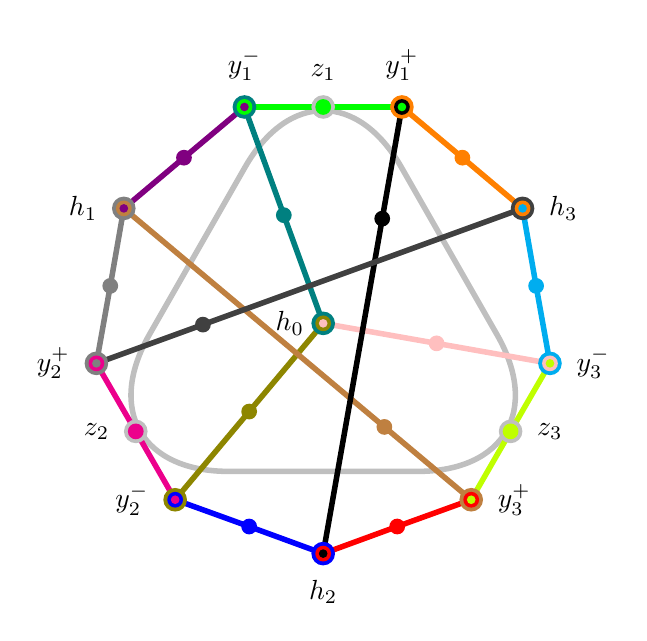
\begin{tikzpicture}  [scale=0.4]

\newdimen\ms
\ms=0.1cm

\tikzstyle{every path}=[line width=2pt]
\tikzstyle{c3}=[circle,inner sep={\ms/8},minimum size=3*\ms]
\tikzstyle{c2}=[circle,inner sep={\ms/8},minimum size=2*\ms]
\tikzstyle{c1}=[circle,inner sep={\ms/8},minimum size=1.1*\ms]



		% Define positions of all observables
		\path
     (-2.50, 6.87    ) coordinate(2)     % $y_1^-
			  (-6.33,   3.65  ) coordinate(4)    % h_1
			  (-7.20, -1.27   ) coordinate(6)       % y_2^+
			  (-4.70, -5.60   ) coordinate(8)       % y_2^-
			  (0, -7.31       ) coordinate(10)       % h_2
			  (4.70, -5.60    ) coordinate(12)        % y_3^+$
     (7.20, -1.27    ) coordinate(14)       % y_3^-
			  (6.33, 3.65     ) coordinate(16)       % h_3
			  (2.50, 6.87     ) coordinate(18)    % y_1^+

			  (0, 6.87        ) coordinate(1)     % z1
			  (-4.42, 5.26    ) coordinate(3)
			  (-6.76, 1.19    ) coordinate(5)
			  (-5.95, -3.43   ) coordinate(7)     % z2
			  (-2.35, -6.45   ) coordinate(9)
     (2.35, -6.45    ) coordinate(11)
			  (5.95,-3.43     ) coordinate(13)    % z3
			  (6.76, 1.19     ) coordinate(15)
		   (4.42, 5.26     ) coordinate(17)

     (0,0) coordinate(19)


(0, 9.3       ) coordinate(20)     % ze1
			  (-8, -4.7    ) coordinate(21)     % ze2
			  (8,-4.7    ) coordinate(22)    % ze3


     (-1.25, 3.435 ) coordinate(23)
     (3.60, -0.635 ) coordinate(24)
     (-2.35, -2.80 ) coordinate(25)
% h1={-6.33,   3.65  }; h3p={4.70, -5.60    } ; h1d2=  (h1+h3p )/2 ; c1=  (h1d2+h3p )/2
     (1.9425, -3.2875) coordinate(26)
% h2={0, -7.31    }; h1p={2.50, 6.87   } ; h2d2=  (h2+h1p )/2 ; c2=  (h2d2+h1p )/2
     (1.875, 3.325) coordinate(27)
% h3={6.33, 3.65    }; h2p={-7.20, -1.27    } ; h3d2=  (h3+h2p )/2 ; c3=  (h3d2+h2p )/2
     (-3.8175, -0.04) coordinate(28)
;

%(4.70-6.33,   3.65  -5.60   ) coordinate(4)    % h_1

	
		% Draw all the context curves
		
\draw [rounded corners=20mm,color=lightgray]     (20) -- (21) -- (22) --  cycle;


\draw [color=green] (18) -- (1) -- (2);
\draw [color=violet] (2) -- (3) -- (4);
\draw [color=gray] (4) -- (5) -- (6);
\draw [color=magenta] (6) -- (7) -- (8);
\draw [color=blue] (8) -- (9) -- (10);
\draw [color=red] (10) -- (11) -- (12) ;

\draw [color=lime] (12) -- (13) -- (14);
\draw [color=cyan] (14) -- (15) -- (16);
\draw [color=orange] (16) -- (17) -- (18);

\draw [color=teal] (19) -- (2);
\draw [color=olive] (19) -- (8);
\draw [color=pink] (19) -- (14);

\draw [color=brown] (4) -- (12);
\draw [color=black] (10) -- (18);
\draw [color=darkgray] (16) -- (6);





%\draw [color=lightgray](0,0) circle (6.87);



\draw (19) coordinate[c3,fill=teal];
\draw (19) coordinate[c2,fill=olive];
\draw (19) coordinate[c1,fill=pink,label=180:$h_0$];


\draw (1)  coordinate[c3,fill=lightgray,label=90:$z_1$];
\draw (1)  coordinate[c2,fill=green];

\draw (2)  coordinate[c3,fill=teal,label=90:$y_1^-$];
\draw (2)  coordinate[c2,fill=green];
\draw (2)  coordinate[c1,fill=violet];

\draw (3)  coordinate[c2,fill=violet];

\draw (4)  coordinate[c3,fill=gray,label=180:$h_1$];
\draw (4)  coordinate[c2,fill=brown];
\draw (4)  coordinate[c1,fill=violet];

\draw (5)  coordinate[c2,fill=gray,label=0:$ $];

\draw (6)  coordinate[c3,fill=darkgray,fill=gray,label=180:$y_2^+$];
\draw (6)  coordinate[c2,fill=magenta];
\draw (6)  coordinate[c1,fill=gray];

\draw (7)  coordinate[c3,fill=lightgray,label=180:$z_2$];
\draw (7)  coordinate[c2,fill=magenta];

\draw (8)  coordinate[c3,fill=olive,label=180:$y_2^-$];
\draw (8)  coordinate[c2,fill=blue];
\draw (8)  coordinate[c1,fill=magenta];

\draw (9)  coordinate[c2,fill=blue,label=0:$ $];

\draw (10) coordinate[c3,fill=blue,label=270:$h_2$];
\draw (10) coordinate[c2,fill=red];
\draw (10) coordinate[c1,fill=black];

\draw (11) coordinate[c2,fill=red,label=0:$ $];

\draw (12) coordinate[c3,fill=brown,label=0:$y_3^+$];
\draw (12) coordinate[c2,fill=red];
\draw (12) coordinate[c1,fill=lime];

\draw (13) coordinate[c3,fill=lightgray,label=0:$z_3$];
\draw (13) coordinate[c2,fill=lime];

\draw (14) coordinate[c3,fill=cyan,label=0:$y_3^-$];
\draw (14) coordinate[c2,fill=pink];
\draw (14) coordinate[c1,fill=lime];

\draw (15) coordinate[c2,fill=cyan,label=0:$ $];

\draw (16) coordinate[c3,fill=darkgray,label=0:$h_3$];
\draw (16) coordinate[c2,fill=orange];
\draw (16) coordinate[c1,fill=cyan];

\draw (17) coordinate[c2,fill=orange,label=0:$ $];

\draw (18) coordinate[c3,fill=orange,label=90:$y_1^+$];
\draw (18) coordinate[c2,fill=black];
\draw (18) coordinate[c1,fill=green];

\draw (23) coordinate[c2,fill=teal];
\draw (24) coordinate[c2,fill=pink];
\draw (25) coordinate[c2,fill=olive];
\draw (26) coordinate[c2,fill=brown];
\draw (27) coordinate[c2,fill=black];
\draw (28) coordinate[c2,fill=darkgray];


		\end{tikzpicture}
&
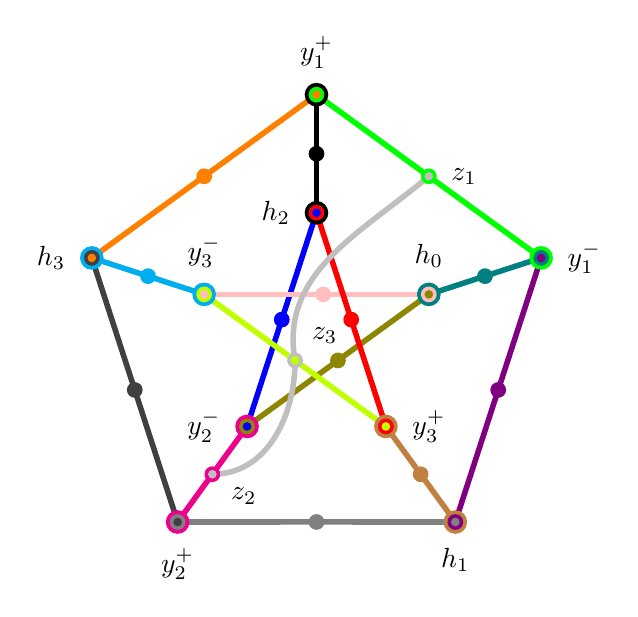
\begin{tikzpicture}  [scale=0.5]
\newdimen\ms
\ms=0.1cm

\tikzstyle{every path}=[line width=2pt]
\tikzstyle{c3}=[circle,inner sep={\ms/8},minimum size=3*\ms]
\tikzstyle{c2}=[circle,inner sep={\ms/8},minimum size=2*\ms]
\tikzstyle{c1}=[circle,inner sep={\ms/8},minimum size=1.1*\ms]

% Radius of regular polygons
\newdimen\R
\R=6cm
%\r= { \R * sqrt(3)/2}
\newdimen\K
\K=3cm

% Define positions of all observables
\path
  ({90 + 0 * 360 /5}:\R      ) coordinate(1)
  ({90 + 360 /10 + 0 * 360/5} : {\R * 0.6881/0.8507} ) coordinate(2)
  ({90 + 1 * 360 /5}:\R   ) coordinate(3)
  ({90 + 360 /10 + 1 * 360/5} : {\R * 0.6881/0.8507} ) coordinate(4)
  ({90 + 2 * 360 /5}:\R  ) coordinate(5)
  ({90 + 360 /10 + 2 * 360/5} : {\R * 0.6881/0.8507} ) coordinate(6)
  ({90 + 3 * 360 /5}:\R  ) coordinate(7)
  ({90 + 360 /10 + 3 * 360/5} : {\R * 0.6881/0.8507} ) coordinate(8)
  ({90 + 4 * 360 /5}:\R     ) coordinate(9)
  ({90 + 360 /10 + 4 * 360/5} : {\R * 0.6881/0.8507} ) coordinate(10)
  ({90 + 0 * 360 /5}:\K      ) coordinate(11)
  ({90 + 360 /10 + 0 * 360/5} : {\K * 0.6881/0.8507} ) coordinate(12)
  ({90 + 1 * 360 /5}:\K   ) coordinate(13)
  ({90 + 360 /10 + 1 * 360/5} : {\K * 0.6881/0.8507} ) coordinate(14)
  ({90 + 2 * 360 /5}:\K  ) coordinate(15)
  ({90 + 360 /10 + 2 * 360/5} : {\K * 0.6881/0.8507} ) coordinate(16)
  ({90 + 3 * 360 /5}:\K  ) coordinate(17)
  ({90 + 360 /10 + 3 * 360/5} : {\R * 0.6881/0.8507} ) coordinate(18)
  ({90 + 4 * 360 /5}:\K     ) coordinate(19)
  ({90 + 360 /10 + 4 * 360/5} : {\K * 0.6881/0.8507} ) coordinate(20)

  ({90 + 2 * 360 /5}:{(\R+\K)/2}) coordinate(21)

;

% draw contexts

\draw [color=orange] (1) -- (2) -- (3);
\draw [color=darkgray] (3) -- (4) -- (5);
\draw [color=gray] (5) -- (6) -- (7);
\draw [color=violet] (7) -- (8) -- (9);
\draw [color=green] (9) -- (10) -- (1);    %

\draw [color=blue] (11) -- (15) ;
\draw [color=olive] (15) -- (19);
\draw [color=pink] (19) -- (13);
\draw [color=lime] (13) -- (17);
\draw [color=red] (17) -- (11);

\draw ($ (11) !.5! (15) $) coordinate[c2,fill=blue];  %
\draw ($ (15) !.5! (19) $) coordinate[c2,fill=olive];  %
\draw ($ (19) !.47! (13) $) coordinate[c2,fill=pink];  %
\draw ($ (17) !.5! (11) $) coordinate[c2,fill=red];  %

\draw [color=black] (1) -- (11);
\draw [color=cyan] (3) -- (13);
\draw [color=magenta] (5) -- (15);
\draw [color=brown] (7) -- (17);
\draw [color=teal] (9) -- (19);

\draw ($ (1) !.5! (11) $) coordinate[c2,fill=black];  %
\draw ($ (3) !.5! (13) $) coordinate[c2,fill=cyan];  %
\draw ($ (7) !.5! (17) $) coordinate[c2,fill=brown];  %
\draw ($ (9) !.5! (19) $) coordinate[c2,fill=teal];  %

\draw [color=lightgray] (10)  to   [out=-140,in=100] ($ (13) !.5! (17) $)  to   [out=-90,in=0] (21);
%
%%
%% draw atoms
%%
%
\draw (1) coordinate[c3,fill=black,label=90:$y_1^+$];  %
\draw (1) coordinate[c2,fill=green];   %
\draw (1) coordinate[c1,fill=orange];  %
%
\draw (2) coordinate[c2,fill=orange];    %
%
\draw (3) coordinate[c3,fill=cyan,label=180:$h_3$];   %
\draw (3) coordinate[c2,fill=darkgray]; %
\draw (3) coordinate[c1,fill=orange];  %
%
\draw (4) coordinate[c2,fill=darkgray];  %
%
\draw (5) coordinate[c3,fill=magenta,label=270:$y_2^+$];  %
\draw (5) coordinate[c2,fill=gray];  %
\draw (5) coordinate[c1,fill=darkgray];  %
%
\draw (6) coordinate[c2,fill=gray];
%
\draw (7) coordinate[c3,fill=brown,label=270:$h_1$];  %
\draw (7) coordinate[c2,fill=violet];  %
\draw (7) coordinate[c1,fill=gray];  %
%
\draw (8) coordinate[c2,fill=violet];  %
%
\draw (9) coordinate[c3,fill=green,label=0:$y_1^-$];
\draw (9) coordinate[c2,fill=teal];
\draw (9) coordinate[c1,fill=violet];  %
%
\draw (10) coordinate[c2,fill=green,label=0:$z_1$];  %
\draw (10) coordinate[c1,fill=lightgray];  %
%
\draw (11) coordinate[c3,fill=black,label=180:$h_2$];  %
\draw (11) coordinate[c2,fill=red];  %
\draw (11) coordinate[c1,fill=blue]; %
%
%
\draw (13) coordinate[c3,fill=cyan,label=90:$y_3^-$]; %
\draw (13) coordinate[c2,fill=lime];  %
\draw (13) coordinate[c1,fill=pink];  %
%
\draw (15) coordinate[c3,fill=magenta,label=180:$y_2^-$]; %
\draw (15) coordinate[c2,fill=olive]; %
\draw (15) coordinate[c1,fill=blue]; %

\draw (17) coordinate[c3,fill=brown,label=0:$y_3^+$];  %
\draw (17) coordinate[c2,fill=red];   %
\draw (17) coordinate[c1,fill=lime]; %

\draw (19) coordinate[c3,fill=teal,label=90:$h_0$]; %
\draw (19) coordinate[c2,fill=pink]; %
\draw (19) coordinate[c1,fill=olive]; %

%
\draw (21) coordinate[c2,fill=magenta];  %
\draw (21) coordinate[c1,fill=lightgray,label=-15:$z_2$];  %

\draw ($ (13) !.5! (17) $) coordinate[c2,fill=lightgray];  %
\draw ($ (13) !.5! (17) $) coordinate[c1,fill=lime,label=45:$z_3$];  %


\end{tikzpicture}
\\
(a)&(b)
\end{tabular}
\end{center}
\caption{\label{2017-b-f-Yu-2012} (Color online) Two equivalent representations of a Petersen graph-like
(with one additional context connecting
$z_1$,
$z_2$, and
$z_3$)
Greechie diagram of the logic considered by Yu and Oh~\cite[Fig.~2]{Yu-2012}.
The set of two-valued states enforces at most one of the four atoms $h_0,h_1,h_2,h_3$ to be 1.
The logic has a (quantum) realization in $\mathbb{R}^3$
consisting of the 25 projections;  associated with the one dimensional subspaces
spanned by  the 13 vectors from the origin $\left(0,0,0\right)^\intercal$ to
$z_1 = \left( 1, 0, 0 \right)^\intercal $,
$z_2 = \left( 0, 1, 0 \right)^\intercal $,
$z_3 = \left( 0, 0, 1 \right)^\intercal $,
$y^-_1 = \left( 0, 1, -1 \right)^\intercal $,
$y^-_2 = \left( 1, 0, -1 \right)^\intercal $,
$y^-_3 = \left( 1, -1, 0 \right)^\intercal $,
$y^+_1 = \left( 0, 1, 1 \right)^\intercal $,
$y^+_2 = \left( 1, 0, 1 \right)^\intercal $,
$y^+_3 = \left( 1, 1, 0 \right)^\intercal $,
$h_0 = \left( 1, 1, 1 \right)^\intercal $,
$h_1 = \left( -1, 1, 1 \right)^\intercal $,
$h_2 = \left( 1, -1, 1 \right)^\intercal $,
$h_3 = \left( 1, 1, -1 \right)^\intercal $,
respectively~\cite{Yu-2012}.
}
\end{figure*}


\subsubsection{Kochen-Specker's $\Gamma_1$ ``true implies true'' logic}
\label{2017-b-s-tit}

A small extension of the Specker bug logic by two contexts extending from $a_1$ and $a_7$,
both intertwining at a point $c$ renders a logic which facilitates that,
whenever $a_1$ is true, so must be an atom $b_1$, which is element in the context $\{a_7,c,b_1\}$,
as depicted in Fig.~\ref{2017-b-f-gamma1}.
\begin{figure}
\begin{center}
%%
%%
%%
%%
%%TexCad Options
%%\grade{\off}
%%\emlines{\off}
%%\beziermacro{\off}
%%\reduce{\on}
%%\snapping{\off}
%%\quality{0.20}
%%\graddiff{0.01}
%%\snapasp{1}
%%\zoom{1.00}
%\unitlength 0.45mm
%%\allinethickness{1pt} %\thicklines %\linethickness{1pt}
%\allinethickness{2pt}
%\begin{picture}(168.00,80.00)
%\put(25.00,7.33){\color{gray}\line(1,0){60.00}}
%\put(25.00,47.33){\color{red}\line(1,0){60.00}}
%\put(55.00,7.33){\color{cyan}\line(0,1){40.00}}
%\put(25.00,7.33){\color{blue}\line(-1,1){20.00}}
%\put(5.00,27.33){\color{green}\line(1,1){20.00}}
%\put(85.00,7.33){\color{magenta}\line(1,1){20.00}}
%\put(105.00,27.33){\color{orange}\line(-1,1){20.00}}
%\put(134.50,27.33){\color{violet}\line(0,-1){20.00}}
%%
%\put(105.00,27.33){\color{pink}\line(1,0){60.00}}
%\put(69, 27.33){\color{violet}\oval(130, 80)[t]}
%%{\color{violet}\qbezier(5,27.33)(32.5,140)(134.76,27.33)}
%%
%\put(134.50,0){\makebox(0,0)[rc]{$b_7$}}
%\put(24.67,55.00){\makebox(0,0)[rc]{$a_3$}}
%\put(55.33,55.00){\makebox(0,0)[cc]{$a_4$}}
%\put(85.33,55.00){\makebox(0,0)[lc]{$a_5$}}
%\put(27.00,37.33){\makebox(0,0)[rc]{$a_2$}}
%\put(99.33,40.00){\makebox(0,0)[lc]{$a_6$}}
%\put(0.00,27.33){\makebox(0,0)[rc]{$a_1$}}
%\put(113.00,32.33){\makebox(0,0)[lc]{$a_7$}}
%\put(60.33,31.33){\makebox(0,0)[lc]{$a_{13}$}}
%\put(9.00,13.33){\makebox(0,0)[rc]{$a_{12}$}}
%\put(99.67,13.33){\makebox(0,0)[lc]{$a_8$}}
%\put(24.67,0){\makebox(0,0)[rc]{$a_{11}$}}
%\put(55.33,0){\makebox(0,0)[cc]{$a_{10}$}}
%\put(85.33,0){\makebox(0,0)[lc]{$a_9$}}
%\put(134.50,7){\color{violet}\circle{1.00}}
%\put(134.50,7){\color{violet}\circle{2.00}}
%\put(15.00,17.09){\color{blue}\circle{1.00}}
%\put(15.00,17.09){\color{blue}\circle{2.00}}
%\put(25.00,7.33){\color{blue}\circle{1.00}}
%\put(25.00,7.33){\color{blue}\circle{2.00}}
%\put(25.00,7.33){\color{gray}\circle{3.00}}
%\put(55.00,27.33){\color{cyan}\circle{1.00}}
%\put(55.00,27.33){\color{cyan}\circle{2.00}}
%\put(85.00,7.33){\color{gray}\circle{1.00}}
%\put(85.00,7.33){\color{gray}\circle{2.00}}
%\put(85.00,7.33){\color{magenta}\circle{3.00}}
%\put(95.00,17.33){\color{magenta}\circle{1.00}}
%\put(95.00,17.33){\color{magenta}\circle{2.00}}
%\put(5.00,27.33){\color{green}\circle{1.00}}
%\put(5.00,27.33){\color{green}\circle{2.00}}
%\put(5.00,27.33){\color{green}\circle{3.00}}
%\put(5.00,27.33){\color{blue}\circle{3.0}}
%\put(5.00,27.33){\color{violet}\circle{5.00}}
%\put(15.00,37.33){\color{green}\circle{1.00}}
%\put(15.00,37.33){\color{green}\circle{2.00}}
%\put(25.00,47.33){\color{green}\circle{1.00}}
%\put(25.00,47.33){\color{green}\circle{2.00}}
%\put(25.00,47.33){\color{red}\circle{3.00}}
%\put(55.00,47.33){\color{red}\circle{1.00}}
%\put(55.00,47.33){\color{red}\circle{2.00}}
%\put(55.00,47.33){\color{cyan}\circle{3.00}}
%\put(85.00,47.33){\color{red}\circle{1.00}}
%\put(85.00,47.33){\color{red}\circle{2.00}}
%\put(85.00,47.33){\color{orange}\circle{3.00}}
%\put(55.00,7.33){\color{gray}\circle{1.00}}
%\put(55.00,7.33){\color{gray}\circle{2.00}}
%\put(55.00,7.33){\color{cyan}\circle{3.00}}
%\put(105,27.33){\color{orange}\circle{1.00}}
%\put(105,27.33){\color{orange}\circle{2.00}}
%\put(105,27.33){\color{magenta}\circle{3.00}}
%\put(105,27.33){\color{pink}\circle{5.00}}
%\put(95.00,37.33){\color{orange}\circle{1.00}}
%\put(95.00,37.33){\color{orange}\circle{2.00}}
%
%\put(165,27.33){\color{pink}\circle{1.00}}
%\put(165,27.33){\color{pink}\circle{2.00}}
%\put(135,27.33){\color{pink}\circle{1.00}}
%\put(134.76,27.33){\color{pink}\circle{2.00}}
%\put(134.76,27.33){\color{violet}\circle{3.00}}
%\put(140.00,32.33){\makebox(0,0)[lc]{$c$}}
%\put(168.00,27.33){\makebox(0,0)[lc]{$b_1$}}
%\end{picture}
%
%
% This is a LaTeX picture output by TeXCAD.
% File name: [1.pic].
% Version of TeXCAD: 4.3
% Reference / build: 30-Jun-2012 (rev. 105)
% For new versions, check: http://texcad.sf.net/
% Options on the following lines.
%\grade{\off}
%\emlines{\off}
%\epic{\off}
%\beziermacro{\on}
%\reduce{\on}
%\snapping{\off}
%\quality{0.200}
%\graddiff{0.010}
%\snapasp{1}
%\zoom{8.0000}
%\unitlength 1mm % = 2.845pt
%\linethickness{0.4pt}
\unitlength 0.55mm
\allinethickness{2pt}
\ifx\plotpoint\undefined\newsavebox{\plotpoint}\fi % GNUPLOT compatibility
\begin{picture}(152,120)(0,0)
%
\put(15.455,85.051){\color{gray}\line(0,-1){60}}
%\put(144.545,85.051){\color{gray}\line(0,-1){60}}
\put(55.455,85.051){\color{red}\line(0,-1){60}}
%\put(104.545,85.051){\color{red}\line(0,-1){60}}
\put(15.455,55.051){\color{cyan}\line(1,0){40}}
%\put(144.545,55.051){\color{cyan}\line(-1,0){40}}
\put(15.455,85.051){\color{blue}\line(1,1){20}}
%\put(144.545,85.051){\color{blue}\line(-1,1){20}}
\put(35.455,105.051){\color{green}\line(1,-1){20}}
%\put(124.545,105.051){\color{green}\line(-1,-1){20}}
\put(15.455,25.051){\color{magenta}\line(1,-1){20}}
%\put(144.545,25.051){\color{magenta}\line(-1,-1){20}}
\put(35.455,5.051){\color{orange}\line(1,1){20}}
%\put(124.545,5.051){\color{orange}\line(-1,1){20}}
%
%
\color{pink}\qbezier(35.5,5.25)(68,5.625)(80,55)
\color{violet}\qbezier(124.5,5.25)(92,5.625)(80,55)
\color{violet}\qbezier(35.5,104.5)(68,104.125)(80,54.75)
\color{pink}\qbezier(124.5,104.5)(92,104.125)(80,54.75)
{\color{black}
%
\put(62.125,80.381){\makebox(0,0)[b]{$a_3$}}
%\put(98.875,80.381){\makebox(0,0)[b]{$b_3$}}
\put(62.125,54.721){\makebox(0,0)[]{$a_4$}}
%\put(98.875,54.721){\makebox(0,0)[]{$b_4$}}
\put(62.125,26.721){\makebox(0,0)[t]{$a_5$}}
%\put(98.875,26.721){\makebox(0,0)[t]{$b_5$}}
\put(43.125,85.051){\makebox(0,0)[b]{$a_2$}}
%\put(116.875,85.051){\makebox(0,0)[b]{$b_2$}}
\put(43.125,22.721){\makebox(0,0)[t]{$a_6$}}
%\put(116.875,22.721){\makebox(0,0)[t]{$b_6$}}
\put(34.455,110.051){\makebox(0,0)[b]{$a_1$}}
 \put(125.545,110.051){\makebox(0,0)[b]{$b_1$}}
\put(34.455,0){\makebox(0,0)[t]{$a_7$}}
 \put(125.545,0){\makebox(0,0)[t]{$b_7$}}
\put(35,49.721){\makebox(0,0)[t]{$a_{13}$}}
%\put(125,49.721){\makebox(0,0)[t]{$b_{13}$}}
\put(21.455,101.051){\makebox(0,0)[b]{$a_{12}$}}
%\put(138.545,101.051){\makebox(0,0)[b]{$b_{12}$}}
\put(21.455,10.381){\makebox(0,0)[t]{$a_8$}}
%\put(138.545,10.381){\makebox(0,0)[t]{$b_8$}}
\put(8.075,85.381){\makebox(0,0)[b]{$a_{11}$}}
%\put(151.925,85.381){\makebox(0,0)[b]{$b_{11}$}}
\put(8.075,54.721){\makebox(0,0)[]{$a_{10}$}}
%\put(151.925,54.721){\makebox(0,0)[]{$b_{10}$}}
\put(8.075,24.721){\makebox(0,0)[t]{$a_9$}}
%\put(151.925,24.721){\makebox(0,0)[t]{$b_9$}}
\put(85,55){\makebox(0,0)[t]{$c$}}
\put(25.215,95.051){\color{blue}\circle{1}}
%\put(134.785,95.051){\color{blue}\circle{1}}
\put(25.215,95.051){\color{blue}\circle{2}}
%\put(134.785,95.051){\color{blue}\circle{2}}
\put(15.455,85.051){\color{blue}\circle{1}}
%\put(144.545,85.051){\color{blue}\circle{1}}
\put(15.455,85.051){\color{blue}\circle{2}}
%\put(144.545,85.051){\color{blue}\circle{2}}
\put(15.455,85.051){\color{gray}\circle{3}}
%\put(144.545,85.051){\color{gray}\circle{3}}
\put(35.455,55.051){\color{cyan}\circle{1}}
%%\put(124.545,55.051){\color{cyan}\circle{1}}
 \put(35.455,55.051){\color{cyan}\circle{2}}
%%\put(124.545,55.051){\color{cyan}\circle{2}}
\put(15.455,25.051){\color{gray}\circle{1}}
%\put(144.545,25.051){\color{gray}\circle{1}}
\put(15.455,25.051){\color{gray}\circle{2}}
%\put(144.545,25.051){\color{gray}\circle{2}}
\put(15.455,25.051){\color{magenta}\circle{3}}
%\put(144.545,25.051){\color{magenta}\circle{3}}
\put(25.455,15.051){\color{magenta}\circle{1}}
%\put(134.545,15.051){\color{magenta}\circle{1}}
\put(25.455,15.051){\color{magenta}\circle{2}}
%\put(134.545,15.051){\color{magenta}\circle{2}}
\put(35.455,105.051){\color{blue}\circle{1}}
%\put(124.545,105.051){\color{blue}\circle{1}}
\put(35.455,105.051){\color{blue}\circle{1}}
%\put(124.545,105.051){\color{blue}\circle{1}}
\put(35.455,105.051){\color{green}\circle{3}}
%\put(124.545,105.051){\color{green}\circle{3}}
\put(35.455,105.051){\color{violet}\circle{5}}
\put(124.545,105){\color{pink}\circle{3}}  %$$$
\put(124.545,105){\color{pink}\circle{1}}  %$$$
\put(45.455,95.051){\color{green}\circle{1}}
%\put(114.545,95.051){\color{green}\circle{1}}
\put(45.455,95.051){\color{green}\circle{2}}
%\put(114.545,95.051){\color{green}\circle{2}}
\put(55.455,85.051){\color{green}\circle{1}}
%\put(104.545,85.051){\color{green}\circle{1}}
\put(55.455,85.051){\color{green}\circle{2}}
%\put(104.545,85.051){\color{green}\circle{2}}
\put(55.455,85.051){\color{red}\circle{3}}
% \put(104.545,85.051){\color{red}\circle{3}}
 \put(55.455,55.051){\color{cyan}\circle{1}}
 %\put(104.545,55.051){\color{cyan}\circle{1}}
 \put(55.455,55.051){\color{cyan}\circle{3}}
 %\put(104.545,55.051){\color{cyan}\circle{1}}
\put(55.455,55.051){\color{red}\circle{3}}
%\put(104.545,55.051){\color{red}\circle{3}}
\put(55.455,25.051){\color{red}\circle{1}}
%\put(104.545,25.051){\color{red}\circle{1}}
\put(55.455,25.051){\color{red}\circle{2}}
%\put(104.545,25.051){\color{red}\circle{2}}
\put(55.455,25.051){\color{orange}\circle{3}}
%\put(104.545,25.051){\color{orange}\circle{3}}
\put(15.455,55.051){\color{cyan}\circle{1}}
%\put(144.545,55.051){\color{cyan}\circle{1}}
\put(15.455,55.051){\color{cyan}\circle{2}}
%\put(144.545,55.051){\color{cyan}\circle{2}}
\put(15.455,55.051){\color{gray}\circle{3}}
%\put(144.545,55.051){\color{gray}\circle{3}}
\put(35.455,5.291){\color{orange}\circle{1}}
%\put(124.545,5.291){\color{orange}\circle{1}}
\put(35.455,5.291){\color{orange}\circle{2}}
%\put(124.545,5.291){\color{orange}\circle{2}}
\put(35.455,5.291){\color{magenta}\circle{3}}
%\put(124.545,5.291){\color{magenta}\circle{3}}
\put(35.455,5.291){\color{pink}\circle{5}}
\put(124.545,5.291){\color{violet}\circle{3}}  %$$$
\put(124.545,5.291){\color{violet}\circle{1}}  %$$$
\put(45.455,15.051){\color{orange}\circle{1}}
%\put(114.545,15.051){\color{orange}\circle{1}}
\put(45.455,15.051){\color{orange}\circle{2}}
%\put(114.545,15.051){\color{orange}\circle{2}}
\put(80,55){\color{pink}\circle{1}}
\put(80,55){\color{violet}\circle{3}}
}
\end{picture}
\end{center}
\caption{\label{2017-b-f-gamma1} (Color online) Greechie diagram of the Kochen-Specker $\Gamma_1$ logic~\cite[p.~68]{kochen1},
which is an extension of the Specker bug logic by two intertwining contexts at the bug's extremities.
The logic has a (quantum) realization in $\mathbb{R}^3$
consisting of the 16 projections associated with the one dimensional subspaces
spanned by  the vectors from the origin $\left(0,0,0\right)^\intercal$ to
the 13 points mentioned in Fig.~\ref{2001-cesena-f2}, as well as
%$a_{1}     = \left(    1,\sqrt{2},0     \right)^\intercal $,
%$a_{2}     = \left(\sqrt{2}, -1, -3 \right)^\intercal $,
%$a_{3}     = \left(   \sqrt{2},-1,1     \right)^\intercal $,
%$a_{4}     = \left(    0,1,1     \right)^\intercal $,
%$a_{5}     = \left(   \sqrt{2},1,-1     \right)^\intercal $,
%$a_{6}     = \left(\sqrt{2}, 1, 3 \right)^\intercal $,
%$a_{7}     = \left(    -1,\sqrt{2},0     \right)^\intercal $,
%$a_{8}     = \left(\sqrt{2}, 1, -3 \right)^\intercal $,
%$a_{9}     = \left(   \sqrt{2},1,1     \right)^\intercal $,
%$a_{10}     = \left(    0,1,-1     \right)^\intercal $,
%$a_{11}     = \left(   \sqrt{2},-1,-1     \right)^\intercal $,
%$a_{12}     = \left(\sqrt{2}, -1, 3 \right)^\intercal $,
%$a_{13}     = \left(    1,0,0     \right)^\intercal $,
 $c          = \left(    0,0,1     \right)^\intercal $,
 $b_{1}     = \left(   \sqrt{2},1,0     \right)^\intercal $,
%$b_{2}     = \left(1, -\sqrt{2}, -3 \right)^\intercal $,
%$b_{3}     = \left(    -1,\sqrt{2},-1     \right)^\intercal $,
%$b_{4}     = \left(    1,0,-1     \right)^\intercal $,
%$b_{5}     = \left(    1,\sqrt{2},1     \right)^\intercal $,
%$b_{6}     = \left(1, \sqrt{2}, -3 \right)^\intercal $,
 $b_{7}     = \left(   \sqrt{2},-1,0     \right)^\intercal $,
%$b_{8}     = \left(1, \sqrt{2}, 3 \right)^\intercal $,
%$b_{9}     = \left(    1,\sqrt{2},-1     \right)^\intercal $,
%$b_{10}     = \left(    1,0,1     \right)^\intercal $,
%$b_{11}     = \left(    -1,\sqrt{2},1     \right)^\intercal $,
%$b_{12}     = \left(-1, \sqrt{2}, -3 \right)^\intercal $,
%$b_{13}     = \left(    0,1,0     \right)^\intercal $,
respectively~\cite[p.~206, Fig.~1]{tkadlec-96}.
}
\end{figure}

The reduction of some probabilities of atoms at intertwined contexts yields
($q_1, q_7$ are the probabilities on $b_1, b_7$, respectively),
additionally to Eq.~(\ref{2015-s-e2}),
\begin{equation}
\begin{split}
p_1 - p_7 = q_1 - q_7
,
\end{split}
\label{2017-b-spa2l}
\end{equation}
which, as  can  be derived also explicitly by taking into account admissibility,
implies that, for all the 112 two-valued states, if $p_1=1$, then [from Eq.~(\ref{2015-s-e2})] $p_7=0$,
and $q_1=1$ as well as $q_7 = 1 - q_1 = 0$.

Besides the  quantum mechanical realization of this logic in terms of propositions identified with projection operators
corresponding to vectors in three-dimensional Hilbert space
Tkadlec and this author~\cite[p.~5387, Fig.~4]{svozil-tkadlec}
(see also Tkadlec~\cite[p.~206, Fig.~1]{tkadlec-96}) have given  an explicit collection of such vectors.
As Tkadlec has observed (cf. Ref.~\cite[p.~5390]{svozil-tkadlec}, and Ref.~\cite[p.]{tkadlec-01}),
the original realization suggested by Kochen and Specker~\cite{kochen1} appears to be a little bit ``buggy''
as they did not use the right angle between $a_1$ and $a_7$, but this can be rectified.

Other ``true implies true'' logics have been introduced by Belinfante~\cite[Fig.~C.l. p.~67]{Belinfante-73},
Pitowsky~\cite[p.~394]{Pitowsky-1982-subs},
Clifton~\cite{clifton-93,Johansen-1994,Vermaas-1994},
as well as Cabello and G. Garc{\'{i}}a-Alcaine~\cite[Lemma~1]{Cabello-1996-bks-fd}.

Notice that, if a second Specker bug logic is placed along $b_1$ and $b_7$,
just as in the Kochen-Specker $\Gamma_3$ logic~\cite[p.~70]{kochen1},
this imposes an additional ``true implies false'' condition; together with the
 ``true implies false'' condition of the first logic this
implies the fact that $a_1$ and $a_7$ can no longer be separated by a two-valued state: whenever one is true,
the other one must be true as well, and {\em vice versa}.
This Kochen-Specker logic $\Gamma_3$ will be discussed in the next Section~\ref{2017-b-bugscombino}.

Notice further that if we manage to iterate this process in such a manner that,
with every $i$th iteration we place another Kochen-Specker $\Gamma_3$ logic  along $b_i$,
while at the same time increasing the angle between $b_i$ and $b_1$,
then eventually we shall arrive at a situation in which $b_1$ and $b_i$ are part of a context
(in terms of Hilbert space: they correspond to orthogonal vectors).
But admissibility disallows two-valued measures with more than one, and in particular,
two ``true'' atoms within a single block. As a consequence, if such a configuration is
realizable (say, in 3-dimensional Hilbert space), then it cannot have any two-valued state
satisfying the admissibility criteria.
This is the Kochen-Specker theorem, as exposed in the  Kochen-Specker $\Gamma_3$ logic~\cite[p.~69]{kochen1},
which will be discussed in Section~\ref{2017-b-c-lwtvs}.


\subsection{Combo of two linked Specker bug logics inducing non-separability}
\label{2017-b-bugscombino}

As we are heading toward  logics with less and less ``rich'' set of two-valued states we are approaching
a logic   depicted in Fig.~\ref{2017-b-f-twobugs}
which is a combination of two Specker bug logics linked by two external contexts.
It is the $\Gamma_3$-configuration of Kochen-Specker~\cite[p.~70]{kochen1}
with a set of two-valued states which is no longer separating:
In this case one obtains the ``one-one'' and ``zero-zero rules''~\cite{svozil-2006-omni},
stating that  $a_1$ occurs if and only if $b_1$ occurs
(likewise, $a_7$ occurs if and only if $b_7$ occurs):
Suppose $v$ is a two-valued state on the $\Gamma_3$-configuration of Kochen-Specker.
Whenever $v(a_1)=1$, then $v(c)=0$ because it is in the same context $\{a_1,c,b_7\}$ as $a_1$.
Furthermore, because of Eq.~(\ref{2015-s-e2}), whenever $v(a_1)=1$, then $v(a_7)=0$.
Because $b_1$ is in the same context $\{a_7,c,b_1\}$ as $a_7$ and $c$, because of admissibility, $v(b_1)=1$.
Conversely, by symmetry, whenever $v(b_1)=1$, so must be $v(a_1)=1$.
Therefore it can never happen that either one of the two atoms $a_1$ and $b_1$ have different dichotomic values.
(Eq.~\ref{2017-b-spa2l} is compatible with these value assignments.)
The same is true for the pair of atoms  $a_7$ and $b_7$.

Note that one needs two Specker bug logics tied together (at their ``true implies false'' extremities)
to obtain non-separability;
just extending one to the
Kochen-Specker $\Gamma_1$ logic~\cite[p.~68]{kochen1} of Fig.~\ref{2017-b-f-gamma1}
discussed earlier to obtain ``true implies true'' would be insufficient.
Because in this case a consistent two-valued state exists for which $v(b_1)=v(b_7)=1$ and $v(a_1)=v(a_7)=0$,
thereby separating $a_1$ from $b_1$, and {\it vice versa}.
A second Specker bug logic is neded to elimitate this case; in particular, $v(b_1)=v(b_7)=1$.


\begin{figure}
\begin{center}
\begin{tabular}{c}
% This is a LaTeX picture output by TeXCAD.
% File name: [1.pic].
% Version of TeXCAD: 4.3
% Reference / build: 30-Jun-2012 (rev. 105)
% For new versions, check: http://texcad.sf.net/
% Options on the following lines.
%\grade{\off}
%\emlines{\off}
%\epic{\off}
%\beziermacro{\on}
%\reduce{\on}
%\snapping{\off}
%\quality{0.200}
%\graddiff{0.010}
%\snapasp{1}
%\zoom{8.0000}
%\unitlength 1mm % = 2.845pt
%\linethickness{0.4pt}
\unitlength 0.55mm
\allinethickness{2pt}
\ifx\plotpoint\undefined\newsavebox{\plotpoint}\fi % GNUPLOT compatibility
\begin{picture}(152,120)(0,0)
%
\put(15.455,85.051){\color{gray}\line(0,-1){60}}
\put(144.545,85.051){\color{gray}\line(0,-1){60}}
\put(55.455,85.051){\color{red}\line(0,-1){60}}
\put(104.545,85.051){\color{red}\line(0,-1){60}}
\put(15.455,55.051){\color{cyan}\line(1,0){40}}
\put(144.545,55.051){\color{cyan}\line(-1,0){40}}
\put(15.455,85.051){\color{blue}\line(1,1){20}}
\put(144.545,85.051){\color{blue}\line(-1,1){20}}
\put(35.455,105.051){\color{green}\line(1,-1){20}}
\put(124.545,105.051){\color{green}\line(-1,-1){20}}
\put(15.455,25.051){\color{magenta}\line(1,-1){20}}
\put(144.545,25.051){\color{magenta}\line(-1,-1){20}}
\put(35.455,5.051){\color{orange}\line(1,1){20}}
\put(124.545,5.051){\color{orange}\line(-1,1){20}}
%
%
\color{pink}\qbezier(35.5,5.25)(68,5.625)(80,55)
\color{violet}\qbezier(124.5,5.25)(92,5.625)(80,55)
\color{violet}\qbezier(35.5,104.5)(68,104.125)(80,54.75)
\color{pink}\qbezier(124.5,104.5)(92,104.125)(80,54.75)
{\color{black}
%
\put(62.125,80.381){\makebox(0,0)[b]{$a_3$}}
\put(98.875,80.381){\makebox(0,0)[b]{$b_3$}}
\put(62.125,54.721){\makebox(0,0)[]{$a_4$}}
\put(98.875,54.721){\makebox(0,0)[]{$b_4$}}
\put(62.125,26.721){\makebox(0,0)[t]{$a_5$}}
\put(98.875,26.721){\makebox(0,0)[t]{$b_5$}}
\put(43.125,85.051){\makebox(0,0)[b]{$a_2$}}
\put(116.875,85.051){\makebox(0,0)[b]{$b_2$}}
\put(43.125,22.721){\makebox(0,0)[t]{$a_6$}}
\put(116.875,22.721){\makebox(0,0)[t]{$b_6$}}
\put(34.455,110.051){\makebox(0,0)[b]{$a_1$}}
\put(125.545,110.051){\makebox(0,0)[b]{$b_1$}}
\put(34.455,0){\makebox(0,0)[t]{$a_7$}}
\put(125.545,0){\makebox(0,0)[t]{$b_7$}}
\put(35,49.721){\makebox(0,0)[t]{$a_{13}$}}
\put(125,49.721){\makebox(0,0)[t]{$b_{13}$}}
\put(21.455,101.051){\makebox(0,0)[b]{$a_{12}$}}
\put(138.545,101.051){\makebox(0,0)[b]{$b_{12}$}}
\put(21.455,10.381){\makebox(0,0)[t]{$a_8$}}
\put(138.545,10.381){\makebox(0,0)[t]{$b_8$}}
\put(8.075,85.381){\makebox(0,0)[b]{$a_{11}$}}
\put(151.925,85.381){\makebox(0,0)[b]{$b_{11}$}}
\put(8.075,54.721){\makebox(0,0)[]{$a_{10}$}}
\put(151.925,54.721){\makebox(0,0)[]{$b_{10}$}}
\put(8.075,24.721){\makebox(0,0)[t]{$a_9$}}
\put(151.925,24.721){\makebox(0,0)[t]{$b_9$}}
\put(85,55){\makebox(0,0)[t]{$c$}}
\put(25.215,95.051){\color{blue}\circle{1}}
\put(134.785,95.051){\color{blue}\circle{1}}
\put(25.215,95.051){\color{blue}\circle{2}}
\put(134.785,95.051){\color{blue}\circle{2}}
\put(15.455,85.051){\color{blue}\circle{1}}
\put(144.545,85.051){\color{blue}\circle{1}}
\put(15.455,85.051){\color{blue}\circle{2}}
\put(144.545,85.051){\color{blue}\circle{2}}
\put(15.455,85.051){\color{gray}\circle{3}}
\put(144.545,85.051){\color{gray}\circle{3}}
 \put(35.455,55.051){\color{cyan}\circle{1}}
 \put(124.545,55.051){\color{cyan}\circle{1}}
 \put(35.455,55.051){\color{cyan}\circle{2}}
 \put(124.545,55.051){\color{cyan}\circle{2}}
\put(15.455,25.051){\color{gray}\circle{1}}
\put(144.545,25.051){\color{gray}\circle{1}}
\put(15.455,25.051){\color{gray}\circle{2}}
\put(144.545,25.051){\color{gray}\circle{2}}
\put(15.455,25.051){\color{magenta}\circle{3}}
\put(144.545,25.051){\color{magenta}\circle{3}}
\put(25.455,15.051){\color{magenta}\circle{1}}
\put(134.545,15.051){\color{magenta}\circle{1}}
\put(25.455,15.051){\color{magenta}\circle{2}}
\put(134.545,15.051){\color{magenta}\circle{2}}
\put(35.455,105.051){\color{blue}\circle{1}}
\put(124.545,105.051){\color{blue}\circle{1}}
\put(35.455,105.051){\color{blue}\circle{1}}
\put(124.545,105.051){\color{blue}\circle{1}}
\put(35.455,105.051){\color{green}\circle{3}}
\put(124.545,105.051){\color{green}\circle{3}}
\put(35.455,105.051){\color{violet}\circle{5}}
\put(124.545,105.051){\color{pink}\circle{5}}
\put(45.455,95.051){\color{green}\circle{1}}
\put(114.545,95.051){\color{green}\circle{1}}
\put(45.455,95.051){\color{green}\circle{2}}
\put(114.545,95.051){\color{green}\circle{2}}
\put(55.455,85.051){\color{green}\circle{1}}
\put(104.545,85.051){\color{green}\circle{1}}
\put(55.455,85.051){\color{green}\circle{2}}
\put(104.545,85.051){\color{green}\circle{2}}
\put(55.455,85.051){\color{red}\circle{3}}
\put(104.545,85.051){\color{red}\circle{3}}
 \put(55.455,55.051){\color{cyan}\circle{1}}
 \put(55.455,55.051){\color{cyan}\circle{3}}
 \put(104.545,55.051){\color{cyan}\circle{1}}
 \put(104.545,55.051){\color{cyan}\circle{3}}
\put(55.455,55.051){\color{red}\circle{3}}
\put(104.545,55.051){\color{red}\circle{3}}
\put(55.455,25.051){\color{red}\circle{1}}
\put(104.545,25.051){\color{red}\circle{1}}
\put(55.455,25.051){\color{red}\circle{2}}
\put(104.545,25.051){\color{red}\circle{2}}
\put(55.455,25.051){\color{orange}\circle{3}}
\put(104.545,25.051){\color{orange}\circle{3}}
\put(15.455,55.051){\color{cyan}\circle{1}}
\put(144.545,55.051){\color{cyan}\circle{1}}
\put(15.455,55.051){\color{cyan}\circle{2}}
\put(144.545,55.051){\color{cyan}\circle{2}}
\put(15.455,55.051){\color{gray}\circle{3}}
\put(144.545,55.051){\color{gray}\circle{3}}
\put(35.455,5.291){\color{orange}\circle{1}}
\put(124.545,5.291){\color{orange}\circle{1}}
\put(35.455,5.291){\color{orange}\circle{2}}
\put(124.545,5.291){\color{orange}\circle{2}}
\put(35.455,5.291){\color{magenta}\circle{3}}
\put(124.545,5.291){\color{magenta}\circle{3}}
\put(35.455,5.291){\color{pink}\circle{5}}
\put(124.545,5.291){\color{violet}\circle{5}}
\put(45.455,15.051){\color{orange}\circle{1}}
\put(114.545,15.051){\color{orange}\circle{1}}
\put(45.455,15.051){\color{orange}\circle{2}}
\put(114.545,15.051){\color{orange}\circle{2}}
\put(80,55){\color{pink}\circle{1}}
\put(80,55){\color{violet}\circle{3}}
}
\end{picture}
\end{tabular}
\end{center}
\caption{\label{2017-b-f-twobugs} (Color online) Greechie diagram of two linked Specker bug (cat's cradle) logics $\Gamma_3$.
The logic has a (quantum) realization in $\mathbb{R}^3$
consisting of the 27 projections associated with the one dimensional subspaces
spanned by  the vectors from the origin $\left(0,0,0\right)^\intercal$ to
the 13 points mentioned in Fig.~\ref{2001-cesena-f2},
the 3 points mentioned in Fig.~\ref{2017-b-f-gamma1}, as well as
%$a_{1}     = \left(    1,\sqrt{2},0     \right)^\intercal $,
%$a_{2}     = \left(\sqrt{2}, -1, -3 \right)^\intercal $,
%$a_{3}     = \left(   \sqrt{2},-1,1     \right)^\intercal $,
%$a_{4}     = \left(    0,1,1     \right)^\intercal $,
%$a_{5}     = \left(   \sqrt{2},1,-1     \right)^\intercal $,
%$a_{6}     = \left(\sqrt{2}, 1, 3 \right)^\intercal $,
%$a_{7}     = \left(    -1,\sqrt{2},0     \right)^\intercal $,
%$a_{8}     = \left(\sqrt{2}, 1, -3 \right)^\intercal $,
%$a_{9}     = \left(   \sqrt{2},1,1     \right)^\intercal $,
%$a_{10}     = \left(    0,1,-1     \right)^\intercal $,
%$a_{11}     = \left(   \sqrt{2},-1,-1     \right)^\intercal $,
%$a_{12}     = \left(\sqrt{2}, -1, 3 \right)^\intercal $,
%$a_{13}     = \left(    1,0,0     \right)^\intercal $,
% $c          = \left(    0,0,1     \right)^\intercal $,
% $b_{1}     = \left(   \sqrt{2},1,0     \right)^\intercal $,
$b_{2}     = \left(1, -\sqrt{2}, -3 \right)^\intercal $,
$b_{3}     = \left(    -1,\sqrt{2},-1     \right)^\intercal $,
$b_{4}     = \left(    1,0,-1     \right)^\intercal $,
$b_{5}     = \left(    1,\sqrt{2},1     \right)^\intercal $,
$b_{6}     = \left(1, \sqrt{2}, -3 \right)^\intercal $,
%$b_{7}     = \left(   \sqrt{2},-1,0     \right)^\intercal $,
$b_{8}     = \left(1, \sqrt{2}, 3 \right)^\intercal $,
$b_{9}     = \left(    1,\sqrt{2},-1     \right)^\intercal $,
$b_{10}     = \left(    1,0,1     \right)^\intercal $,
$b_{11}     = \left(    -1,\sqrt{2},1     \right)^\intercal $,
$b_{12}     = \left(-1, \sqrt{2}, -3 \right)^\intercal $,
$b_{13}     = \left(    0,1,0     \right)^\intercal $,
respectively~\cite[p.~206, Fig.~1]{tkadlec-96}.
Note that, with this realization, there is an additional context $\{ a_{13},c,b_{13}\}$ not drawn here,
which imposes an additional constraint $v(a_{13})+v(c)+v(b_{13})=1$ on any two-valued measure $v$.
(See also the proof of Proposition~7.2 in Ref.~\cite[p.~5392]{svozil-tkadlec}.)
}
\end{figure}

Besides the  quantum mechanical realization of this logic in terms of propositions which are projection operators
corresponding to vectors in three-dimensional Hilbert space suggested by Kochen and Specker~\cite{kochen1},
Tkadlec has given~\cite[p.~206, Fig.~1]{tkadlec-96}  an explicit collection of such vectors
(see also the proof of Proposition~7.2 in Ref.~\cite[p.~5392]{svozil-tkadlec}).


\subsubsection{Probabilistic criteria against value definiteness from constraints on two-valued measures}
\label{2017-b-ss-pc}

The ``1-1'' or  ``true implies true'' rule can be taken as an operational criterion for quantization:
Suppose that one prepares a system to be in a pure state
corresponding to $a_1$, such that the preparation ensures that $v(a_1)=1$.
If the system is then measured along $b_1$, and the proposition that
the system is in state $b_1$  is found  to be {\em not} true, meaning that $v(b_1)\neq 1$ (the respective detector does not click),
then  one has established that the system is not performing classically,
because classically the set of two-valued states requires non-separability; that is, $v(a_1)=v(b_1)=1$.
With the Tkadlec directions taken from Figs.~\ref{2001-cesena-f2} and~\ref{2017-b-f-gamma1},
$\vert {\bf a}_1\rangle = (1/\sqrt{3}) \left(    1,\sqrt{2},0     \right)^\intercal$ and
$\vert {\bf b}_1\rangle = (1/\sqrt{3})\left(     \sqrt{2},1,0      \right)^\intercal$
so that the probability to find a quantized system prepared along $\vert {\bf a}_1\rangle$
and measured along $\vert {\bf b}_1\rangle$ is
$p_{a_1}(b_1) = \vert \langle {\bf b}_1 \vert {\bf a}_1 \rangle \vert^2=  8/9  $,
and that a violation of classicality should occur with probability $1/9$.
Of course, any other classical prediction, such as the ``1-0'' or ``true implies false'' rule,
or more general  classical predictions such as of Eq.~(\ref{2015-s-e2})
can also be taken as empirical criteria for non-classicality~\cite[Sect.~11.3.2.]{svozil-2016-s}).

Indeed, already Stairs~\cite[p.~588-589]{stairs83} has argued along similar lines for the Specker bug
``true implies false'' logic (a translation into our nomenclature
is:
$m1(1) \equiv a_1$,
$m2(1) \equiv a_3$,
$m2(2) \equiv a_5$,
$m2(3) \equiv a_4$,
$m3(1) \equiv a_{11}$,
$m3(2) \equiv a_9$,
$m3(3) \equiv a_{10}$,
$m4(1) \equiv a_7$).
Independently Clifton (there is a note added in proof to Stairs~\cite[p.~588-589]{stairs83})
presents asimilar argument, based upon (i) another ``true implies true'' logic~\cite[Sects.~II,III, Fig.~1]{clifton-93,Johansen-1994,Vermaas-1994}
inspired by Bell~\cite[Fig.~C.l. p.~67]{Belinfante-73} (cf. also Pitowsky~\cite[p.~394]{Pitowsky-1982-subs}),
as well as (ii) on the Specker bug logic~\cite[Sects.~IV, Fig.~2]{clifton-93}.
More recently Hardy~\cite{Hardy-92,Hardy-93,hardy-97}
as well as Cabello and
Garc{\'{i}}a-Alcaine and
others~\cite{Cabello-1995-ppks,cabello-96,cabello-97-nhvp,Badziag-2011,Cabello-2013-HP,Cabello-2013-Hardylike} discussed such scenarios.
These criteria for non-classicality are benchmarks aside from the Boole-Bell type polytope method,
and also different from the full Kochen-Specker theorem.


\subsubsection{Imbedability}

As every algebra imbeddable in a Boolean algebra must have a separating set of two valued states,
this logic is no longer ``classical''
in the sense of ``homomorphically (structure-preserving) imbeddable.''
Nevertheless, two-valued states can still exist. It is just that these states can no longer differentiate
between the pairs of atoms $(a_1,b_1)$ as well as $(a_7,b_7)$.
Partition logics and their generalized urn or finite automata models fail to reproduce
two linked Specker bug logics resulting in a Kochen-Specker $\Gamma_3$ logic even at this stage.
Of course, the situation will become more dramatic with the non-existence of any kind of two-valued state
(interpretable as truth assignment) on certain logics associate with quantum propositions.

Complementarity and non-distributivity is not enough to characterize logics which do not have a quasi-classical
(partition logical, set theoretical) interpretation.
While in a certain, graph coloring sense the ``richness/scarcity'' and the {\em ``number''
of two-valued homomorphisms''} yields insights into the old problem of the structural property~\cite{Cooke-1983}
by
separating quasi-classical from quantum logics,
the problem of finding smaller, maybe minimal,
subsets of graphs with a non-separating set of two-valued states  still remains an open challenge.

\subsubsection{Chromatic inseparability}

The ``true implies true'' rule is associated with
{\em chromatic separability};
\index{chromatic separability}
in particular, with the impossibility to separate two atoms $a_7$ and $b_7$
with less than four colors.
A proof is presented in Fig.~\ref{2017-b-f-twobugschromaticsep}.
That chromatic separability on the unit sphere requires 4 colors  is implicit in Refs.~\cite{godsil-zaks,havlicek-2000}.
\begin{figure}
\begin{center}
\begin{tabular}{c}
% This is a LaTeX picture output by TeXCAD.
% File name: [1.pic].
% Version of TeXCAD: 4.3
% Reference / build: 30-Jun-2012 (rev. 105)
% For new versions, check: http://texcad.sf.net/
% Options on the following lines.
%\grade{\off}
%\emlines{\off}
%\epic{\off}
%\beziermacro{\on}
%\reduce{\on}
%\snapping{\off}
%\quality{0.200}
%\graddiff{0.010}
%\snapasp{1}
%\zoom{8.0000}
%\unitlength 1mm % = 2.845pt
%\linethickness{0.4pt}
\unitlength 0.55mm
\allinethickness{2pt}
\ifx\plotpoint\undefined\newsavebox{\plotpoint}\fi % GNUPLOT compatibility
\begin{picture}(152,120)(0,-1)
%
\put(15.455,85.051){\color{gray}\line(0,-1){60}}
\put(144.545,85.051){\color{gray}\line(0,-1){60}}
\put(55.455,85.051){\color{red}\line(0,-1){60}}
\put(104.545,85.051){\color{red}\line(0,-1){60}}
 \put(15.455,55.051){\color{cyan}\line(1,0){40}}
 \put(144.545,55.051){\color{cyan}\line(-1,0){40}}
\put(15.455,85.051){\color{blue}\line(1,1){20}}
\put(144.545,85.051){\color{blue}\line(-1,1){20}}
\put(35.455,105.051){\color{green}\line(1,-1){20}}
\put(124.545,105.051){\color{green}\line(-1,-1){20}}
\put(15.455,25.051){\color{magenta}\line(1,-1){20}}
\put(144.545,25.051){\color{magenta}\line(-1,-1){20}}
\put(35.455,5.051){\color{orange}\line(1,1){20}}
\put(124.545,5.051){\color{orange}\line(-1,1){20}}
%
%
\color{pink}\qbezier(35.5,5.25)(68,5.625)(80,55)
\color{violet}\qbezier(124.5,5.25)(92,5.625)(80,55)
\color{violet}\qbezier(35.5,104.5)(68,104.125)(80,54.75)
\color{pink}\qbezier(124.5,104.5)(92,104.125)(80,54.75)
{\color{black}
%
%\put(62.125,80.381){\makebox(0,0)[b]{$a_3$}}
%\put(98.875,80.381){\makebox(0,0)[b]{$b_3$}}
\put(65.125,54.721){\makebox(0,0)[]{$a_4$}}
\put(95.875,54.721){\makebox(0,0)[]{$b_4$}}
%\put(62.125,26.721){\makebox(0,0)[t]{$a_5$}}
%\put(98.875,26.721){\makebox(0,0)[t]{$b_5$}}
%\put(43.125,85.051){\makebox(0,0)[b]{$a_2$}}
%\put(116.875,85.051){\makebox(0,0)[b]{$b_2$}}
%\put(43.125,22.721){\makebox(0,0)[t]{$a_6$}}
%\put(116.875,22.721){\makebox(0,0)[t]{$b_6$}}
\put(34.455,110.051){\makebox(0,0)[b]{$a_1$}}
\put(125.545,110.051){\makebox(0,0)[b]{$b_1$}}
\put(34.455,-1){\makebox(0,0)[t]{$a_7$}}
\put(125.545,-1){\makebox(0,0)[t]{$b_7$}}
%\put(35,49.721){\makebox(0,0)[t]{$a_{13}$}}
%\put(125,49.721){\makebox(0,0)[t]{$b_{13}$}}
%\put(21.455,101.051){\makebox(0,0)[b]{$a_{12}$}}
%\put(138.545,101.051){\makebox(0,0)[b]{$b_{12}$}}
%\put(21.455,10.381){\makebox(0,0)[t]{$a_8$}}
%\put(138.545,10.381){\makebox(0,0)[t]{$b_8$}}
%\put(8.075,85.381){\makebox(0,0)[b]{$a_{11}$}}
%\put(151.925,85.381){\makebox(0,0)[b]{$b_{11}$}}
\put(5.075,54.721){\makebox(0,0)[]{$a_{10}$}}
\put(155.925,54.721){\makebox(0,0)[]{$b_{10}$}}
%\put(8.075,24.721){\makebox(0,0)[t]{$a_9$}}
%\put(151.925,24.721){\makebox(0,0)[t]{$b_9$}}
\put(88,55){\makebox(0,0)[t]{$c$}}
%\put(25.215,95.051){\color{blue}\circle{1}}
%\put(134.785,95.051){\color{blue}\circle{1}}
%\put(25.215,95.051){\color{blue}\circle{2}}
%\put(134.785,95.051){\color{blue}\circle{2}}
%\put(15.455,85.051){\color{blue}\circle{1}}
%\put(144.545,85.051){\color{blue}\circle{1}}
%\put(15.455,85.051){\color{blue}\circle{2}}
%\put(144.545,85.051){\color{blue}\circle{2}}
%\put(15.455,85.051){\color{gray}\circle{3}}
%\put(144.545,85.051){\color{gray}\circle{3}}
%\put(35.455,55.051){\color{cyan}\circle{1}}
%\put(124.545,55.051){\color{cyan}\circle{1}}
%\put(35.455,55.051){\color{cyan}\circle{2}}
%\put(124.545,55.051){\color{cyan}\circle{1}}
%\put(124.545,55.051){\color{cyan}\circle{2}}
%\put(15.455,25.051){\color{gray}\circle{1}}
%\put(144.545,25.051){\color{gray}\circle{1}}
%\put(15.455,25.051){\color{gray}\circle{2}}
%\put(144.545,25.051){\color{gray}\circle{2}}
%\put(15.455,25.051){\color{magenta}\circle{3}}
%\put(144.545,25.051){\color{magenta}\circle{3}}
%\put(25.455,15.051){\color{magenta}\circle{1}}
%\put(134.545,15.051){\color{magenta}\circle{1}}
%\put(25.455,15.051){\color{magenta}\circle{2}}
%\put(134.545,15.051){\color{magenta}\circle{2}}
 \put(35.455,105.051){\color{red}\circle{1}}
 \put(124.545,105.051){\color{green}\circle{1}}
 \put(35.455,105.051){\color{red}\circle{2}}
 \put(124.545,105.051){\color{green}\circle{1}}
 \put(35.455,105.051){\color{red}\circle{3}}
 \put(124.545,105.051){\color{green}\circle{3}}
 \put(35.455,105.051){\color{red}\circle{5}}
 \put(35.455,105.051){\color{red}\circle{7}}
 \put(124.545,105.051){\color{green}\circle{5}}
 \put(124.545,105.051){\color{green}\circle{7}}
%\put(45.455,95.051){\color{green}\circle{1}}
%\put(114.545,95.051){\color{green}\circle{1}}
%\put(45.455,95.051){\color{green}\circle{2}}
%\put(114.545,95.051){\color{green}\circle{2}}
%\put(55.455,85.051){\color{green}\circle{1}}
%\put(104.545,85.051){\color{green}\circle{1}}
%\put(55.455,85.051){\color{green}\circle{2}}
%\put(104.545,85.051){\color{green}\circle{2}}
%\put(55.455,85.051){\color{red}\circle{3}}
%\put(104.545,85.051){\color{red}\circle{3}}
 \put(55.455,55.051){\color{red}\circle{1}}
 \put(55.455,55.051){\color{red}\circle{2}}
 \put(55.455,55.051){\color{red}\circle{3}}
 \put(55.455,55.051){\color{red}\circle{5}}
 \put(55.455,55.051){\color{red}\circle{7}}
 \put(104.545,55.051){\color{green}\circle{1}}
 \put(104.545,55.051){\color{green}\circle{2}}
 \put(104.545,55.051){\color{green}\circle{3}}
 \put(104.545,55.051){\color{green}\circle{5}}
 \put(104.545,55.051){\color{green}\circle{7}}
%\put(55.455,25.051){\color{red}\circle{1}}
%\put(104.545,25.051){\color{red}\circle{1}}
%\put(55.455,25.051){\color{red}\circle{2}}
%\put(104.545,25.051){\color{red}\circle{2}}
%\put(55.455,25.051){\color{orange}\circle{3}}
%\put(104.545,25.051){\color{orange}\circle{3}}
 \put(15.455,55.051){\color{red}\circle{1}}
 \put(15.455,55.051){\color{red}\circle{2}}
 \put(15.455,55.051){\color{red}\circle{3}}
 \put(15.455,55.051){\color{red}\circle{5}}
 \put(15.455,55.051){\color{red}\circle{7}}
 \put(144.545,55.051){\color{green}\circle{2}}
  \put(144.545,55.051){\color{green}\circle{5}}
  \put(144.545,55.051){\color{green}\circle{3}}
  \put(144.545,55.051){\color{green}\circle{1}}
  \put(144.545,55.051){\color{green}\circle{7}}
 \put(35.455,5.291){\color{red}\circle{1}}
 \put(35.455,5.291){\color{red}\circle{2}}
 \put(35.455,5.291){\color{red}\circle{3}}
 \put(35.455,5.291){\color{red}\circle{5}}
 \put(35.455,5.291){\color{red}\circle{7}}
 \put(124.545,5.291){\color{green}\circle{3}}
 \put(124.545,5.291){\color{green}\circle{2}}
 \put(124.545,5.291){\color{green}\circle{1}}
 \put(124.545,5.291){\color{green}\circle{5}}
 \put(124.545,5.291){\color{green}\circle{7}}
%\put(45.455,15.051){\color{orange}\circle{1}}
%\put(114.545,15.051){\color{orange}\circle{1}}
%\put(45.455,15.051){\color{orange}\circle{2}}
%\put(114.545,15.051){\color{orange}\circle{2}}
 \put(80,55){\color{blue}\circle{1}}
 \put(80,55){\color{blue}\circle{3}}
 \put(80,55){\color{blue}\circle{5}}
 \put(80,55){\color{blue}\circle{7}}
}
\end{picture}
\end{tabular}
\end{center}
\caption{\label{2017-b-f-twobugschromaticsep} (Color online) Proof (by contradiction) that chromatic separability
of two linked Specker bug (cat's cradle) logics $\Gamma_3$ cannot be achieved with three colors.
In particular, $a_7$ and $b_7$ cannot be separated, as this would result in the depicted inconsistent coloring:
suppose a red/green/blue coloring  with chromatic admissibility (``all three colors occur only once per context or block orBoolean subalgebra'')
is possible.
Then, if
$a_7$ is colored red
and
$b_7$ is colored green,
$c$ must be colored blue.
Therefore,
$a_1$ must be colored red.
Therefore,
$a_4$ as well as $a_{10}$
must be colored red (similar for green on the second Specker bug),
contradicting admissibility.
}
\end{figure}




\subsection{Propositional structures without two-valued states}
\label{2017-b-c-lwtvs}

 %\input 2017-b-ch-pswtvs.tex
% 2017-b-ch-pswtvs


%\subsection{Propositional structures without two-valued states}
%\label{2017-b-c-lwtvs}

\subsubsection{Gleason-type continuity}
\label{2017-b-c-lwtvs-gleason}

Gleason's theorem~\cite{Gleason} was a response to Mackey's
problem to {\em ``determine all measures on the closed subspaces of a Hilbert space''} contained in a review~\cite{ma-57} of
Birkhoff and von Neumann's centennial paper~\cite{birkhoff-36} on the logic of quantum mechanics.
Starting from von Neumann's formalization of quantum mechanics~\cite{v-neumann-49,v-neumann-55},
the quantum mechanical probabilities and expectations
(aka the Born rule)
are essentially derived from (sub)additivity
among the quantum context; that is, from subclassicality:
within any context (Boolean subalgebra, block, maximal observable, orthonormal base)
the quantum probabilities sum up to $1$.

Gleason's finding caused ripples in the community,
at least of those who cared and coped with
it~\cite{ZirlSchl-65,kamber65,bell-66,kochen1,c-k-m,r:dvur-93,pitowsky:218,rich-bridge}.
(I recall having an argument with Van Lambalgen around 1983, who could not believe that anyone in the larger quantum community
had not heard of Gleason's theorem.
As we approached an elevator at Vienna University of Technology's Freihaus building we realized there was also one very prominent
member of Vienna experimental community entering the cabin.
I suggested to stage an example by asking; and {\em voila}$\ldots$)

With the possible exception of Specker who did not explicitly refer to the Gleason's theorem
in independently announcing that two-valued states on quantum logics cannot exist~\cite{specker-60}
-- he must have made up his mind from other arguments and preferred to discuss scholastic philosophy;
at that time the Swiss may have had their own biotope --
Gleason's theorem directly implies the absence of two-valued states.
Indeed, at least for finite dimensions~\cite{Alda,Alda2},
as Zierler and Schlessinger~\cite[p.~259, Example~3.2]{ZirlSchl-65} (even before publication of Bell's review~\cite{bell-66}) noted,
 {\em ``it should also be mentioned that, in fact, the non-existence of two-valued states is an elementary
geometric fact contained quite explicitly in~\cite[Paragraph~2.8]{Gleason}.''}

Now, Gleason's Paragraph~2.8 contains the following main (necessity) theorem~\cite[p.~888]{Gleason}:
{\em ``Every non-negative frame function on the unit sphere $S$ in ${\Bbb R}^3$
ir regular.''}
Whereby~\cite[p.~886]{Gleason}
{\em ``a frame function $f$ [[satisfying additivity]]
is regular if and only if there exists a self-adjoint
operator $\textsf{\textbf{T}}$ defined on [[the separable Hilbert space]] $\mathfrak{H}$ such that
$f( \vert x \rangle ) = \langle \textsf{\textbf{T}}x \vert x\rangle$ for all unit vectors $ \vert x \rangle $.''}
(Of course, Gleason did not use the Dirac notation.)

In what follows we shall consider Hilbert spaces of dimension $n=3$ and higher.
Suppose that the quantum system is prepared to be in a
pure state associated with the unit vector $\vert x \rangle$,
or the projection operator $\vert x \rangle \langle x \vert$.

As all self-adjoint operators have a spectral decomposition~\cite[{\S}~79]{halmos-vs},
and the scalar product is (anti)linear in its arguments,
let us, instead of $\textsf{\textbf{T}}$, only consider one-dimensional orthogonal projection operators
$\textsf{\textbf{E}}_i^2=\textsf{\textbf{E}}_i = \vert y_i \rangle \langle y_i \vert$
(formed by the unit vector $ \vert y_i \rangle $ which are elements of an orthonormal basis
$\{  \vert y_1 \rangle , \ldots ,  \vert y_n \rangle \}$)
occurring in the spectral sum of
$\textsf{\textbf{T}}=\sum_{i=1}^{n\ge 3} \lambda_i \textsf{\textbf{E}}_i$,
with
${\Bbb I}_n =\sum_{i=1}^{n\ge 3} \textsf{\textbf{E}}_i$.

Thus if $\textsf{\textbf{T}}$ is restricted to some one-dimensional projection operator
$\textsf{\textbf{E}} = \vert y \rangle \langle y \vert$ along $\vert y \rangle $,
then Gleason's main theorem
states that any frame function
reduces to the absolute square of the scalar product;
and in real Hilbert space to the square of the angle between those vectors spanning the linear subspaces corresponding to the two projectors involved;
that is (note that $\textsf{\textbf{E}}$ is self-adjoint),
$f_y( \vert x \rangle ) =
\langle \textsf{\textbf{E}}x \vert x\rangle  =
\langle x \vert \textsf{\textbf{E}} x\rangle  =
\langle x \vert y \rangle \langle y \vert x\rangle  =
\vert \langle x \vert y \rangle
\vert^2 = \cos^2 \angle (x,y)$.
%This frame function is identified with the probability on some propositions encoded by projection operators.

Hence, unless a configuration of contexts is not of the star-shaped Greechie orthogonality diagram form
--
meaning that they all share one common atom; and,
in terms of geometry, meaning that all orthonormal bases share a common vector
--
and the two-valued state has value $1$ on its centre, as depicted in Fig.~\ref{2017-b-c-notvsstar},
there is no way how any two contexts could have a two-valued assignment; even if one context has one: it is just not possible by the continuous, $\cos^2$-form
of the quantum probabilities.
That is (at least in this author's believe) the watered down version of the remark of Zierler and Schlessinger~\cite[p.~259, Example~3.2]{ZirlSchl-65}.
\begin{figure}
\begin{center}
% This is a LaTeX picture output by TeXCAD.
% File name: [2.pic].
% Version of TeXCAD: 4.3
% Reference / build: 30-Jun-2012 (rev. 105)
% For new versions, check: http://texcad.sf.net/
% Options on the following lines.
%\grade{\on}
%\emlines{\off}
%\epic{\off}
%\beziermacro{\on}
%\reduce{\on}
%\snapping{\off}
%\pvinsert{% Your \input, \def, etc. here}
%\quality{8.000}
%\graddiff{0.005}
%\snapasp{1}
%\zoom{8.0000}
\unitlength 0.4mm % = 2.845pt
\allinethickness{2pt}
\ifx\plotpoint\undefined\newsavebox{\plotpoint}\fi % GNUPLOT compatibility
\begin{picture}(110,110)(40,40)
\put(100,100){\color{red}\line(-1,0){60}}
\put(100,100){\color{green}\line(0,1){60}}
\put(100,100){\color{blue}\line(1,0){60}}
\put(100,100){\color{orange}\line(0,-1){60}}
%\put(40,100){\circle{4}}
%\put(100,160){\circle{4}}
%\put(160,100){\circle{4}}
%\put(40,100){\circle{4}}
%\put(100,160){\circle{4}}
%\put(100,40){\circle{4}}
%\put(70,100){\circle{4}}
%\put(100,130){\circle{4}}
%\put(130,100){\circle{4}}
%\put(100,70){\circle{4}}
\put(100,100){\color{magenta}\line(-1,-1){42.5}}
\put(100,100){\color{pink}\line(1,1){42.5}}
\put(100,100){\color{cyan}\line(1,-1){42.5}}
%\emline(100,100)(44.5,77.25)
\multiput(100,100)(-.08222222222,-.0337037037){675}{\color{lightgray}\line(-1,0){.08222222222}}
%\end
%\emline(100,100)(155.5,122.75)
\multiput(100,100)(.08222222222,.0337037037){675}{\color{gray}\line(1,0){.08222222222}}
%\end
%\emline(100,100)(77.25,155.5)
\multiput(100,100)(-.0337037037,.08222222222){675}{\color{brown}\line(0,1){.08222222222}}
%\end
%\emline(100,100)(122.75,44.5)
\multiput(100,100)(.0337037037,-.08222222222){675}{\color{yellow}\line(0,-1){.08222222222}}
%\end
%\emline(100,100)(77,44.5)
\multiput(100,100)(-.03372434018,-.08137829912){682}{\color{red}\line(0,-1){.08137829912}}
%\end
%\emline(100,100)(123,155.5)
\multiput(100,100)(.03372434018,.08137829912){682}{\color{purple}\line(0,1){.08137829912}}
%\end
%\emline(100,100)(155.5,77)
\multiput(100,100)(.08137829912,-.03372434018){682}{\color{violet}\line(1,0){.08137829912}}
%\end
%\put(72.25,88.5){\circle{4}}
%\put(127.75,111.5){\circle{4}}
%\put(88.5,127.75){\circle{4}}
%\put(111.5,72.25){\circle{4}}
%\put(78.75,78.75){\circle{4}}
%\put(121.25,121.25){\circle{4}}
%\put(121.25,78.75){\circle{4}}
%\put(88.5,72.25){\circle{4}}
%\put(111.5,127.75){\circle{4}}
%\put(127.75,88.5){\circle{4}}
%\put(44.25,76.75){\circle{4}}
%\put(155.75,123.25){\circle{4}}
%\put(76.75,155.75){\circle{4}}
%\put(123.25,44.25){\circle{4}}
%\put(57.5,57.75){\circle{4}}
%\put(142.5,142.25){\circle{4}}
%\put(142.25,57.5){\circle{4}}
%\put(77,44.5){\circle{4}}
%\put(123,155.5){\circle{4}}
%\put(155.5,77){\circle{4}}
\put(75.25,116.375){\circle*{2}}
\put(79.875,122.125){\circle*{2}}
\put(71.875,109.875){\circle*{2}}
\put(100,100){\circle*{10}}
\end{picture}
\end{center}
\caption{\label{2017-b-c-notvsstar} (Color online) Greechie diagram of a star shaped configuration with a variety of contexts,
all intertwined in a single ``central'' atom; with overlaid two-valued state (bold black filled circle)
which is one on the centre atom and zero everywhere else (see also Refs.~\cite{2012-incomput-proofsCJ,PhysRevA.89.032109,2015-AnalyticKS}).}
\end{figure}


\subsubsection{Finite logics admitting no two-valued states}

When it comes to the absence of a global two-valued state on quantum logics corresponding to Hilbert
spaces of dimension three and higher -- where contexts or blocks can be intertwined or pasted~\cite{nav:91} to form chains --
Kochen and Specker~\cite{kochen1} pursued a very concrete, ``constructive''
(in the sense of finitary mathematical objects but not in the sense of physical operationalizability~\cite{bridgman})
strategy: they presented finite logics realizable by vectors (from the origin to the unit sphere) spanning one-dimensional subspaces, equivalent
to observable propositions, which allowed for lesser \& lesser two-valued state properties.
For the reason of non-imbedability is is already enough
to consider two linked Specker bugs logics $\Gamma_3$~\cite[p.~70]{kochen1}, as
discussed in Sect.~\ref{2017-b-bugscombino}.

Kochen and Specker went further and presented a  proof by contradiction
of the non-existence of two-valued states on a finite number of propositions,
based on their  $\Gamma_1$ ``true implies true'' logic~\cite[p.~68]{kochen1} discussed in Sect.~\ref{2017-b-f-gamma1},
iterating them until they reached a complete contradiction in their $\Gamma_2$ logic~\cite[p.~69]{kochen1}.
As has been pointed out earlier, their representation as points of the sphere is a little bit ``buggy'' (as could be expected from the formation of so many bugs):
as Tkadlec has observed, Kochen-Specker diagram $\Gamma_2$ it is not a one-to-one representation of the logic, because some different points
at the diagram represent the same element of corresponding orthomodular
poset (cf. Ref.~\cite[p.~5390]{svozil-tkadlec}, and Ref.~\cite[p.]{tkadlec-01}).

The early 1990's saw an ongoing flurry of papers recasting the Kochen-Specker proof with ever smaller numbers of,
or more symmetric, configurations of
observables
(see Refs.~\cite{peres-91,penrose-ks,Peres:1996fk,Kernaghan-1994,mermin-93,bub,svozil-tkadlec,tkadlec-96,cabello-96,Cabello-1996ega,CalHerSvo-tatra,tkadlec-00,tkadlec-01,pavicic:inria-00070615,Smith-2004,Pavicic-2005,Arends2011,Waegell-2011,1751-8121-44-50-505303,Planat2012,PhysRevLett.108.030402,Cabello-2014-PhysRevA.89.042101} for an incomplete list).
Arguably the most compact such logic is one in four-dimensional space suggested by Cabello, Estebaranz and Garc{\'{i}}a-Alcaine~\cite{cabello-96,cabello-99,Pavicic-2005}.
It consists of 9 contexts, with each of the 18 atoms tightly intertwined in two contexts.
Its Greechie orthogonality diagram is drawn in Fig.~\ref{2016-pu-book-chapter-qm-f-kspac}.
\begin{figure}
\begin{center}
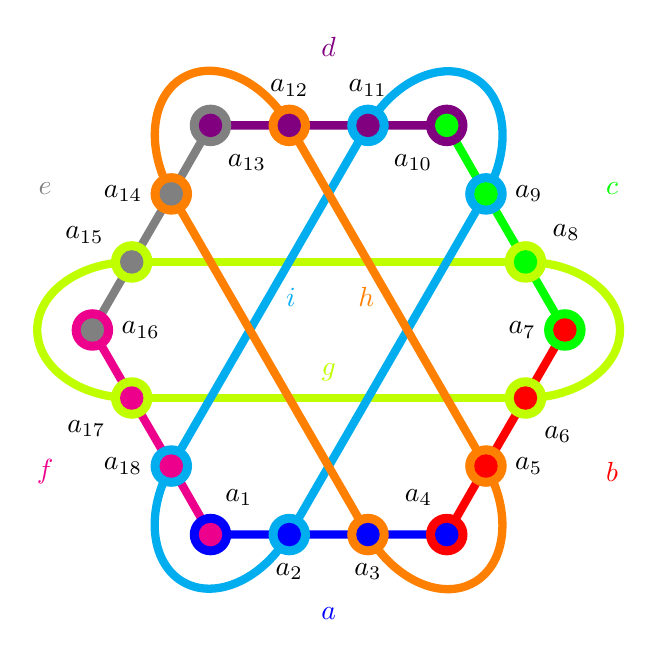
\begin{tikzpicture}  [scale=0.6]

		\tikzstyle{every path}=[line width=3pt]
		\tikzstyle{c2}=[circle,inner sep=3pt,minimum size=15pt]
		\tikzstyle{c1}=[circle,inner sep=3pt,minimum size=0pt]
		%\tikzstyle{s1}=[rectangle,minimum size=9]
		\tikzstyle{l1}=[draw=none,circle,minimum size=35]
		\tikzstyle{l2}=[draw=none,circle,minimum size=12]

		% Define positions of all observables
		\path
			  (240:5) coordinate(1)
			  (-0.833,-4.33) coordinate(2)
			  (0.833,-4.33) coordinate(3)
			  (300:5) coordinate(4)
			  (3.33,-2.88) coordinate(5)
			  (4.167,-1.44) coordinate(6)
     (0:5) coordinate(7)
			  (4.167,1.44) coordinate(8)
			  (3.33,2.88) coordinate(9)
		      (60:5) coordinate(10)
			  (0.833,4.33) coordinate(11)
			  (-0.833,4.33) coordinate(12)
			  (120:5) coordinate(13)
			  (-3.33,2.88) coordinate(14)
			  (-4.167,1.44) coordinate(15)
			  (180:5) coordinate(16)
			  (-4.167,-1.44) coordinate(17)
			  (-3.33,-2.88) coordinate(18);

\node[draw=none,color=blue] at (0,-6) {$a$};
\node[draw=none,color=red] at (6,-3) {$b$};
\node[draw=none,color=green] at (6,3) {$c$};
\node[draw=none,color=violet] at (0,6) {$d$};
\node[draw=none,color=gray] at (-6,3) {$e$};
\node[draw=none,color=magenta] at (-6,-3) {$f$};
\node[draw=none,color=cyan] at (-0.8,0.7) {$i$};
\node[draw=none,color=orange] at (0.8,0.7) {$h$};
\node[draw=none,color=lime] at (0,-0.9) {$g$};


	
		% Draw all the context curves
		\draw [color=green] (7) -- (8) -- (9)-- (10);
\draw [color=violet] (10) -- (11) -- (12) -- (13);
\draw [color=gray] (13) -- (14) -- (15) -- (16);
\draw [color=magenta] (16) -- (17) -- (18) -- (1);
\draw [color=blue] (1) -- (2) -- (3) -- (4);
\draw [color=red] (4) -- (5) -- (6) -- (7);

		\draw [color=lime] (8) -- (15);
		\draw [color=lime](17) -- (6);
		\draw [color=lime] (8) arc (450:270:2 and 1.44);
		\draw [color=lime] (15) arc (90:270:2 and 1.44);

		\draw [color=cyan] (9) -- (2);
		\draw [color=cyan] (11) -- (18);
		\draw [rotate=240,color=cyan] (9) arc (90:270:2 and 1.44);
		\draw[rotate=60,color=cyan] (18) arc (90:270:2 and 1.44);

		\draw [color=orange] (12) -- (5);
		\draw [color=orange] (14) -- (3);
		\draw[rotate=300,color=orange] (12) arc (90:270:2 and 1.44);
		\draw[rotate=120,color=orange] (3) arc (90:270:2 and 1.44);

		% Draw the observables themselves
		\draw (1) coordinate[c2,fill=blue];
		\draw (1) coordinate[c1,fill=magenta,label=85:$a_1$];
		\draw (2) coordinate[c2,fill=cyan];
		\draw (2) coordinate[c1,fill=blue,label=270:$a_2$];
\draw (3) coordinate[c2,fill=orange];
		\draw (3) coordinate[c1,fill=blue,label=270:$a_3$];
		\draw (4) coordinate[c2,fill=red];
		\draw (4) coordinate[c1,fill=blue,label=95:$a_4$];
\draw (5) coordinate[c2,fill=orange];
		\draw (5) coordinate[c1,fill=red,label=0:$a_5$];
\draw (6) coordinate[c2,fill=lime];
		\draw (6) coordinate[c1,fill=red,label=290:$a_6$];
		\draw (7) coordinate[c2,fill=green];
		\draw (7) coordinate[c1,fill=red,label=180:$a_7$];
\draw (8) coordinate[c2,fill=lime];
		\draw (8) coordinate[c1,fill=green,label=30:$a_8$];
\draw (9) coordinate[c2,fill=cyan];
		\draw (9) coordinate[c1,fill=green,label=0:$a_9$];
		\draw (10) coordinate[c2,fill=violet];
		\draw (10) coordinate[c1,fill=green,label=265:$a_{10}$];
\draw (11) coordinate[c2,fill=cyan];
		\draw (11) coordinate[c1,fill=violet,label=91:$a_{11}$];
\draw (12) coordinate[c2,fill=orange];
		\draw (12) coordinate[c1,fill=violet,label=90:$a_{12}$];
		\draw (13) coordinate[c2,fill=gray];
		\draw (13) coordinate[c1,fill=violet,label=285:$a_{13}$];
\draw (14) coordinate[c2,fill=orange];
		\draw (14) coordinate[c1,fill=gray,label=180:$a_{14}$];
\draw (15) coordinate[c2,fill=lime];
		\draw (15) coordinate[c1,fill=gray,label=160:$a_{15}$];
		%%\draw (15) node[c1,fill=none] {\Huge $\times$};
		%\draw (15) coordinate[s1,fill,label=150:$P_c$];
		%\draw (15) coordinate[c1,fill=white];
		%%\draw (15) coordinate[c1,draw];
		\draw (16) coordinate[c2,fill=magenta];
		\draw (16) coordinate[c1,fill=gray,label=0:$a_{16}$];
\draw (17) coordinate[c2,fill=lime];
		\draw (17) coordinate[c1,fill=magenta,label=215:$a_{17}$];
\draw (18) coordinate[c2,fill=cyan];
		\draw (18) coordinate[c1,fill=magenta,label=180:$a_{18}$];

		% Context labels
		%\coordinate[l1,label=260:$C_1$] (c1) at (16);
		%\coordinate[l2,label=25:$C_2$] (c2) at (16);
	\end{tikzpicture}
\end{center}
\caption{(Color online)
The most compact way of deriving the Kochen-Specker theorem in four dimensions has been given by
Cabello, Estebaranz and Garc{\'{i}}a-Alcaine~\cite{cabello-96}.
The configuration consists of 18 biconnected (two contexts intertwine per atom)
atoms $a_1, \ldots , a_{18}$ in 9 contexts.
It has a (quantum) realization in $\mathbb{R}^4$
consisting of the 18 projections associated with the one dimensional subspaces spanned by
the vectors from the origin $(0,0,0,0)^\intercal$ to
$a_1=\left(   0,0,1,-1     \right)^\intercal    $,
$a_2=\left(   1,-1,0,0     \right)^\intercal    $,
$a_3=\left(   1,1,-1,-1    \right)^\intercal   $,
$a_4=\left(   1,1,1,1      \right)^\intercal     $,
$a_5=\left(   1,-1,1,-1    \right)^\intercal  $,
$a_6=\left(   1,0,-1,0     \right)^\intercal   $,
$a_7=\left(   0,1,0,-1   \right)^\intercal   $,
$a_8=\left(   1,0,1,0    \right)^\intercal    $,
$a_9=\left(   1,1,-1,1   \right)^\intercal   $,
$a_{10}=\left(-1,1,1,1   \right)^\intercal    $,
$a_{11}=\left(1,1,1,-1   \right)^\intercal    $,
$a_{12}=\left(1,0,0,1    \right)^\intercal     $,
$a_{13}=\left(0,1,-1,0   \right)^\intercal    $,
$a_{14}=\left(0,1,1,0    \right)^\intercal    $,
$a_{15}=\left(0,0,0,1    \right)^\intercal    $,
$a_{16}=\left(1,0,0,0    \right)^\intercal    $,
$a_{17}=\left(0,1,0,0    \right)^\intercal    $,
$a_{18}=\left(0,0,1,1    \right)^\intercal    $,
 respectively~\cite[Fig.~1]{cabello:210401}
(for alternative realizations see Refs.~\cite{cabello-99,cabello:210401}).
%
\label{2016-pu-book-chapter-qm-f-kspac}
}
\end{figure}

In a parity proof by contradiction
consider the particular subset of real four-dimensional Hilbert space with a ``parity property,''
\index{parity property}
consisting of 18 atoms $a_1, \ldots , a_{18}$ in 9 contexts,
as depicted in Figure~\ref{2016-pu-book-chapter-qm-f-kspac}.
Note that, on the one hand,
each atom/point/vector/projector belongs
to exactly two -- that is, an {\em even} number of -- contexts; that is, it is biconnected.
Therefore,
%in order to obey non-contextuality -- in particular, the independence of any value of a two-valued state on the context it belongs to --
any enumeration of  all the contexts occurring in the graph
depicted in Figure~\ref{2016-pu-book-chapter-qm-f-kspac}
would contain an {\em even} number of $1$s assigned.
Because, due to non-contextuality and biconnectivity,
any atom $a$ with $v(a)=1$ along one context must have the same value 1 along the second context
which is intertwined with the first one -- to the values 1 appear in pairs.

Alas, on the other hand, in such an enumeration
there are nine  -- that is, an {\em odd} number of -- contexts.
Hence,
in order to obey the quantum predictions,
any  two-valued state (interpretable as truth assignment)
would need to have an {\em odd} number of $1$s -- exactly one for each context.
Therefore, there cannot exist any two-valued state on Kochen-Specker type graphs with the  ``parity property.''
%https://arxiv.org/pdf/1702.05215.pdf

More concretely,  note that, within each one of those 9 contexts,
the sum of any state on the atoms of that context must add up to 1.
That is, due to additivity (\ref{2017-ch-pu-qlff}) and (\ref{2017-ch-pu-glff})
one obtains a system of 9 equations
\begin{equation}
\begin{split}
\color{blue}        v(a)= v( a_1 ) + v( a_2 ) + v( a_3 ) + v( a_4 ) = 1 ,                  \\
\color{red}         v(b)= v( a_4 ) + v( a_5 ) + v( a_6 ) + v( a_7 ) = 1 ,                  \\
\color{green}       v(c)= v( a_7 ) + v( a_8 ) + v( a_9 ) + v( a_{10} ) = 1 ,               \\
\color{violet}      v(d)= v( a_{10} ) + v( a_{11} ) + v( a_{12} ) + v( a_{13} ) = 1 ,      \\
\color{gray}        v(e)= v( a_{13} ) + v( a_{14} ) + v( a_{15} ) + v( a_{16} ) = 1 ,      \\
\color{magenta}     v(f)= v( a_{16} ) + v( a_{17} ) + v( a_{18} ) + v( a_1 ) = 1 ,         \\
\color{lime}        v(g)= v( a_6 ) + v( a_8 ) + v( a_{15} ) + v( a_{17} ) = 1 ,            \\
\color{orange}      v(h)= v( a_3 ) + v( a_5 ) + v( a_{12} ) + v( a_{14} ) = 1 ,            \\
\color{cyan}        v(i)= v( a_2 ) + v( a_9 ) + v( a_{11} ) + v( a_{18} ) = 1 .
\label{2017-b-e-cabp-conf}
\end{split}
\end{equation}
By summing up the left hand side and the right hand sides of the equations, and since all atoms are biconnected,
one obtains
\begin{equation}
2 \left[\sum_{i=1}^{18} v(a_i)\right] = 9.
\label{2017-b-e-cabp}
\end{equation}
Because $v(a_i)\in \{0,1\}$ the sum in (\ref{2017-b-e-cabp}) must add up to some natural number $M$.
Therefore, Eq.~(\ref{2017-b-e-cabp}) is impossible to solve in the domain of natural numbers,
as on the left and right hand sides there appear even ($2M$) and odd ($9$) numbers, respectively.

Of course, one could also prove the nonexistence of any  two-valued state (interpretable as truth assignment)
by exhaustive attempts
(possibly exploiting symmetries) to assign values $0$s and $1$s to the atoms/points/vectors/projectors occurring in the graph
in such a way that both the quantum predictions as well as context independence is satisfied.
This latter method needs to be applied in cases with Kochen-Specker type diagrams without the  ``parity property;''
such as in the original Kochen-Specker proof~\cite{kochen1}.
(However, admissibility (IV) is too weak for a proof of this type,
as it allows also a third, value indefinte, state, which spoils the arguments~\cite{2015-AnalyticKS}.)

This result, as well as the original Kochen-Specker theorem,
is {\em state independent} insofar as it applies to an arbitrary quantum state.
One could {\em reduce the size of the proof} by assuming a particular state. Such proofs are called
{\em state-specific} or {\em state dependent.}
By following  Cabello, Estebaranz and Garc{\'{i}}a-Alcaine~\cite[Eqs.~(10)-(19), p.~185]{cabello-96}
their state independent proof utilizing the logic depicted in Fig.~\ref{2016-pu-book-chapter-qm-f-kspac}
can be transferred to a state-specific proof as follows:
suppose that the quantum (or quanta, depending upon the physical realization) is prepared in the state
\begin{equation}
v(a_1) = 1,
\label{2017-b-e-cabp2}
\end{equation}
so that any two-valued state must obey the admissibility rules
\begin{equation}
v(a_2)=v(a_3)=v(a_4)=v(a_{16}) =v(a_{17})=v(a_{18}) =0.
\label{2017-b-e-cabp3}
\end{equation}
The additivity relations~(\ref{2017-b-e-cabp-conf}) reduce to seven equations (two equations encoding contexts
${\color{blue}a}$ and ${\color{magenta}f}$ are satisfied trivially)
\begin{equation}
\begin{split}
\color{red}         v(b')=  v( a_5 ) + v( a_6 ) + v( a_7 ) = 1 ,                  \\
\color{green}       v(c)= v( a_7 ) + v( a_8 ) + v( a_9 ) + v( a_{10} ) = 1 ,               \\
\color{violet}      v(d)= v( a_{10} ) + v( a_{11} ) + v( a_{12} ) + v( a_{13} ) = 1 ,      \\
\color{gray}        v(e')= v( a_{13} ) + v( a_{14} ) + v( a_{15} ) = 1 ,      \\
\color{lime}        v(g')=  v( a_6 ) + v( a_8 ) + v( a_{15} ) = 1 ,            \\
\color{orange}      v(h')=  v( a_5 ) + v( a_{12} ) + v( a_{14} ) = 1 ,            \\
\color{cyan}        v(i')=  v( a_9 ) + v( a_{11} )  = 1 .
\label{2017-b-e-cabp-conf2}
\end{split}
\end{equation}
The configuration is depicted in Fig.~\ref{2016-pu-book-chapter-qm-f-kspac2}.
As all atoms remain to be biconnected and there are 7, that is,  an odd number, of equations, value
indefiniteness can be proven by a similar parity argument as before.
One could argue that the ``primed'' contexts in (\ref{2017-b-e-cabp-conf2}) are not complete
because those contexts are ``truncated.''
However, every completion would result in vectors orthogonal to $a_1$;
and therefore their values must again be zero.
\begin{figure}
\begin{center}
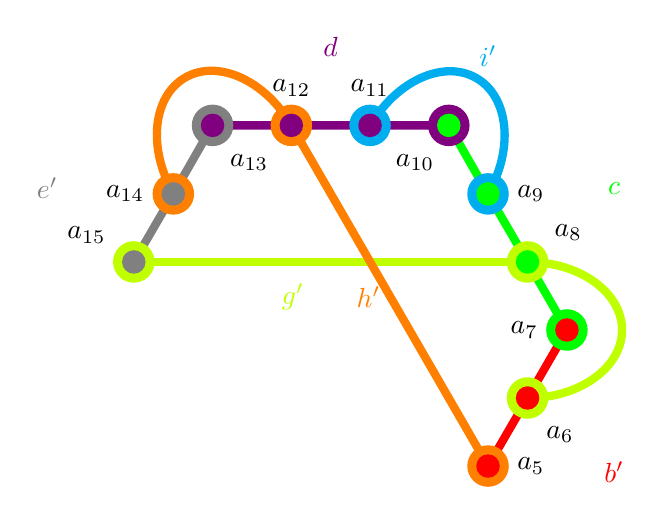
\begin{tikzpicture}  [scale=0.6]
		\tikzstyle{every path}=[line width=3pt]
		\tikzstyle{c2}=[circle,inner sep=3pt,minimum size=15pt]
		\tikzstyle{c1}=[circle,inner sep=3pt,minimum size=0pt]
		%\tikzstyle{s1}=[rectangle,minimum size=9]
		\tikzstyle{l1}=[draw=none,circle,minimum size=35]
		\tikzstyle{l2}=[draw=none,circle,minimum size=12]

		% Define positions of all observables
		\path
			  (3.33,-2.88) coordinate(5)
			  (4.167,-1.44) coordinate(6)
     (0:5) coordinate(7)
			  (4.167,1.44) coordinate(8)
			  (3.33,2.88) coordinate(9)
		      (60:5) coordinate(10)
			  (0.833,4.33) coordinate(11)
			  (-0.833,4.33) coordinate(12)
			  (120:5) coordinate(13)
			  (-3.33,2.88) coordinate(14)
			  (-4.167,1.44) coordinate(15);

%\node[draw=none,color=blue] at (0,-6) {$a$};
\node[draw=none,color=red] at (6,-3) {$b'$};
\node[draw=none,color=green] at (6,3) {$c$};
\node[draw=none,color=violet] at (0,6) {$d$};
\node[draw=none,color=gray] at (-6,3) {$e'$};
%\node[draw=none,color=magenta] at (-6,-3) {$f$};
\node[draw=none,color=cyan] at (3.33,5.8) {$i'$};
\node[draw=none,color=orange] at (0.8,0.7) {$h'$};
\node[draw=none,color=lime] at (-0.8,0.7) {$g'$};


	
		% Draw all the context curves
		\draw [color=green] (7) -- (8) -- (9)-- (10);
\draw [color=violet] (10) -- (11) -- (12) -- (13);
\draw [color=gray] (13) -- (14) -- (15) ;
%\draw [color=magenta] (16) -- (17) -- (18) -- (1);
%\draw [color=blue] (1) -- (2) -- (3) -- (4);
\draw [color=red] (5) -- (6) -- (7);

  \draw [color=lime] (8) -- (15);
%	\draw [color=lime](17) -- (6);
		\draw [color=lime] (8) arc (450:270:2 and 1.44);
%	\draw [color=lime] (15) arc (90:270:2 and 1.44);

%		\draw [color=cyan] (9) -- (2);
%		\draw [color=cyan] (11) -- (18);
  	\draw [rotate=240,color=cyan] (9) arc (90:270:2 and 1.44);
%		\draw[rotate=60,color=cyan] (18) arc (90:270:2 and 1.44);

		\draw [color=orange] (12) -- (5);
%	\draw [color=orange] (14) -- (3);
		\draw[rotate=300,color=orange] (12) arc (90:270:2 and 1.44);
%	\draw[rotate=120,color=orange] (3) arc (90:270:2 and 1.44);

		% Draw the observables themselves
\draw (5) coordinate[c2,fill=orange];
		\draw (5) coordinate[c1,fill=red,label=0:$a_5$];
\draw (6) coordinate[c2,fill=lime];
		\draw (6) coordinate[c1,fill=red,label=290:$a_6$];
		\draw (7) coordinate[c2,fill=green];
		\draw (7) coordinate[c1,fill=red,label=180:$a_7$];
\draw (8) coordinate[c2,fill=lime];
		\draw (8) coordinate[c1,fill=green,label=30:$a_8$];
\draw (9) coordinate[c2,fill=cyan];
		\draw (9) coordinate[c1,fill=green,label=0:$a_9$];
		\draw (10) coordinate[c2,fill=violet];
		\draw (10) coordinate[c1,fill=green,label=265:$a_{10}$];
\draw (11) coordinate[c2,fill=cyan];
		\draw (11) coordinate[c1,fill=violet,label=91:$a_{11}$];
\draw (12) coordinate[c2,fill=orange];
		\draw (12) coordinate[c1,fill=violet,label=90:$a_{12}$];
		\draw (13) coordinate[c2,fill=gray];
		\draw (13) coordinate[c1,fill=violet,label=285:$a_{13}$];
\draw (14) coordinate[c2,fill=orange];
		\draw (14) coordinate[c1,fill=gray,label=180:$a_{14}$];
\draw (15) coordinate[c2,fill=lime];
		\draw (15) coordinate[c1,fill=gray,label=160:$a_{15}$];
		%%\draw (15) node[c1,fill=none] {\Huge $\times$};
		%\draw (15) coordinate[s1,fill,label=150:$P_c$];
		%\draw (15) coordinate[c1,fill=white];
		%%\draw (15) coordinate[c1,draw];

		% Context labels
		%\coordinate[l1,label=260:$C_1$] (c1) at (16);
		%\coordinate[l2,label=25:$C_2$] (c2) at (16);
	\end{tikzpicture}
\end{center}
\caption{(Color online)
Greechie orthogonality diagram of a state-specific proof of the Kochen-Specker theorem
based on the assumption that the physical system is  in state $a_1$, such that $v(a_1)=1$.
The additivity and admissibility constraints  (\ref{2017-b-e-cabp-conf2}) represent different ``reduced'' (or ``truncated'') contexts,
because all states $v(a_2)=v(a_3)=v(a_4)=v(a_{16}) =v(a_{17})=v(a_{18}) =0$ ``orthogonal to'' $a_1$ must vanish.
\label{2016-pu-book-chapter-qm-f-kspac2}
}
\end{figure}



\subsubsection{Chromatic number of the sphere}

Graph coloring allows another view on value (in)definiteness.
The {\em chromatic number} of a graph
\index{chromatic number}
is defined as the least number of colors needed in any total coloring of a graph;
with the constraint that two adjacent vertices have distinct colors.

Suppose that we are interested in the chromatic number of graphs associated with
both (i) the real and (ii) the rational three-dimensional unit sphere.
%defined by
%$S^3 =
%\big\{ \vert {\bf x} \rangle \big|  \vert {\bf x} \rangle =
%\begin{pmatrix}
%x_1,x_2,x_3
%\end{pmatrix}^\intercal
%, \;
%x_1^2+x_2^2+x_3^2=1, \; x_1,x_2,x_3 \in \mathbb{R}
%\big\}
%$,
%as well as $S^3\cap \mathbb{Q}^3$, respectively.

More generally, we can consider $n$-dimensional unit spheres with the same adjacency property defined by orthogonality.
An orthonormal basis will be called context (block, maximal observable, Boolean subalgebra),
or, in this particular area, a $n$-clique.
Note that for any such graphs involving $n$-cliques the chromatic number of this graph is at least be $n$
(because the chromatic number of a single $n$-clique or context is $n$).

Thereby vertices of the graph are identified with points on the three-dimensional unit sphere;
with adjacency  defined by orthogonality; that is,
two vertices of the graph are adjacent if and only if the unit vectors from the origin
to the respective two points are orthogonal.

The connection to quantum logic is this: any context
(block, maximal observable, Boolean subalgebra, orthonormal basis)
can be represented by a triple of points on the sphere
such that any two unit vectors from the origin
to two distinct points of that triple of points are orthogonal.
Thus graph adjacency in logical terms indicates
``belonging to some common context (block, maximal observable, Boolean subalgebra, orthonormal basis).''

In three dimensions, if the chromatic number of  graphs is four or higher,
there does not globally exist any consistent
coloring obeying the rule that adjacent vertices (orthogonal vectors)
must have different colors: if one allows only three different colors,
then somewhere in that graph of chromatic number higher than three, adjacent vertices must have the same colors
(or else the chromatic number would be three or lower).


By a similar argument, non-separability of two-valued states
--
such as encountered in Section~\ref{2017-b-bugscombino}
with the $\Gamma_3$-configuration of Kochen-Specker~\cite[p.~70]{kochen1}
-- translates into non-differentiability by colorings
with colors less or equal to the number of atoms in a block
(cf. Fig.~\ref{2017-b-f-twobugschromaticsep}).

Godsil and Zaks~\cite{godsil-zaks,havlicek-2000}  proved the following results:
\begin{enumerate}
\item
the chromatic number of the graph based on points of real-valued unit sphere
is four~\cite[Lemma~1.1]{godsil-zaks}.
\item
The chromatic number of rational points on the  unit sphere
$S^3\cap \mathbb{Q}^3$
is three~\cite[Lemma~1.2]{godsil-zaks}.
\end{enumerate}

We shall concentrate on (i) and discuss (ii) later.
As has been pointed out by Godsil in an email conversation from March 13, 2016~\cite{godsil-pc},
{\em ``the fact that the chromatic number of the unit sphere in $\mathbb{R}^3$
is four is a consequence of  Gleason's theorem,
from which the Kochen-Specker theorem follows by compactness.
Gleason's result implies that there is no subset of the sphere that contains exactly one point from each orthonormal basis.''}

Indeed, any coloring can be mapped onto a two-valued state by identifying
a single color with ``$1$'' and all other colors with ``$0$.''
By reduction, all propositions on two-valued states translate into statements about graph coloring.
In particular, if the chromatic number of any logical structure representable as graph consisting of $n$-atomic
contexts
(blocks, maximal observables with $n$ outcomes, Boolean subalgebras $2^n$, orthonormal bases with $n$ elements)
--
for instance, as Greechie orthogonality diagram of quantum logics
--
is larger than $n$,
then there cannot be any globally consistent two-valued state (truth value assignment) obeying adjacency (aka admissibility).
Likewise, if no two-valued states  on a logic
which is a pasting of $n$-atomic contexts
exist, then, by reduction, no global consistent coloring with $n$ different colors exists.
Therefore, the Kochen-Specker theorem proves that the chromatic number of the graph corresponding to
the unit sphere with adjacency defined as orthogonality must be higher than three.




%\subsubsection{Breaking up intertwines}

Based on Godsil and Zaks finding that the chromatic number of rational points on the  unit sphere
$S^3\cap \mathbb{Q}^3$
is three~\cite[Lemma~1.2]{godsil-zaks} -- thereby constructing a two-valued measure on the rational unit sphere
by identifying one color with ``$1$'' and the two remaining colors with ``$0$'' --
there exist ``exotic'' options to circumvent Kochen-Specker type constructions which have been quite aggressively (Cabello has referred to this
as the {\em second contextuality war} \cite{Cabello-talk-Vajo-2017})
marketed by allegedly ``nullifying''~\cite{meyer:99} the respective theorems
under the umbrella of ``finite precision measurements''~\cite{kent:99,clifton:99,mermin-99iks,Breuer-02a,Breuer-02b,Barrett-2004}:
the support of vectors spanning the one-dimensional subspaces associated with atomic propositions could be ``diluted'' yet dense,
so much so that the intertwines of contexts (blocks, maximal observables, Boolean subalgebras, orthonormal bases) break up;
and the contexts themselves become ``free \& isolated.''
Under such circumstances the logics decay into horizontal sums;
and the Greechie orthogonality diagrams are just disconnected stacks of previously intertwined contexts.
As can be expected, proofs of Gleason- or Kochen-Specker-type theorems do no longer exist,
as the necessary intertwines are missing.

%More concretely,
%one could consider all unit vectors with the
%{\em Pythagorean property}
%$i^2+j^2+k^2=n^2$ for $i,j,k \in \mathbb{Z}, n \in \mathbb{N}$;
%that is,
%\begin{equation}
%\begin{split}
%\Big\{ \vert {\bf x} \rangle \Big|  \vert {\bf x} \rangle =
%\begin{pmatrix}
%\frac{i}{n},\frac{j}{n},\frac{k}{n}
%\end{pmatrix}^\intercal
%,
%i,j,k,n \in \mathbb{Z} \setminus \left\{\left(0,0,0\right)^\intercal \right\}, \\
%i^2+j^2+k^2=n^2
%\Big\}  = S^3\cap \mathbb{Q}^3
%\end{split}
%\end{equation}
%encodes all rational points
%on the unit sphere.
%This can be verified by writing any rational point on the unit sphere as
%$   \vert {\bf r} \rangle =
%\begin{pmatrix}
%\frac{a}{a'},\frac{b}{b'},\frac{c}{c'}
%\end{pmatrix}^\intercal
%$  with
%$a,b,c\in \mathbb{Z}$ and
%$a',b',c'\in \mathbb{Z} \setminus \left\{ 0 \right\}$,
%with
%$
%\left(\frac{a}{a'}\right)^2 + \left(\frac{b}{b'}\right)^2 + \left(\frac{c}{c'}\right)^2 =1
%$.
%Multiplying $\vert {\bf r} \rangle$  with
%with ${a'}{b'}{c'}$
%yields a vector satisfying the Pythagorean property
%$
%({a }{b'}{c'})^2 +
%({a'}{b }{c'})^2 +
%({a'}{b'}{c })^2=
%({a'}{b'}{c'})^2
%$.

The ``nullification'' claim and subsequent ones triggered a lot of papers, some cited in ~\cite{Barrett-2004};
mostly critical -- of course, not to the results of Godsil and Zaks's finding (ii); how could they? -- but to their physical applicability.
Peres even wrote a parody by arguing that  {\em ``finite precision measurement nullifies Euclid's postulates''}~\cite{peres-2003-fpnep},
so that ``nullification'' of the Kochen-Specker theorem might have to be our least concern.
%Rather than presenting a detailed formal discussion I shall mention an anecdote: shortly after
%the publication of ``nullification'' paper~\cite{meyer:99} Specker called me up in Vienna.
%He was quite upset and suggested
%(in German; translated from my memory):
%{\em ``I need not be directly involved in this; but you should write a response to that paper.''}
%
%So I conceived a reply (now partially contained in~\cite{havlicek-2000}) --
%basically criticising that, in such a configuration, every neighborhood of points on the sphere
%would have to be colored with all three colors; and thus, by identification, the resulting probability measure (frame function)
%would be highly discontinuous -- a discontinuity which is not encountered in actual experiment;
%as well as the absence of closedness under fundamental logical processes.
%
%After councellation with Specker we submitted a comment
%which met the highest resistance in the peer review processes of two journals ({\em Physical Review Letters} and {\em Physics Letters A})
%which rejected the manuscript.
%One referee pointed out that {\em ``the usual meaning of the phrase ``Kochen-Specker
%        theorem'' is not quite what the authors state''}
%(thereby basically unknowingly alleging that Specker did not know what his own theorem was about).
%Another, final, referee  remarked that
%{\em ``the authors' first criticism of Meyer seems to me perverse.''}

%Specker's typical reaction in a personal email messages from June 20th, 2000~\cite{Specker-priv-June2000},
%with reference to~\cite{clifton:99},
%was,
%{\em that a dense set $M$ of directions exist in $n$-dimensional space with the property that
%no two directions in $M$ are orthogonal, that is completely evident (assuming some familiarity
%in topology and recursive constructions).
%Of course, for such directions no problems exist with regards to imbedability.
%If that appears too trivial, a dense set of directions can be constructed such that every direction
%belongs to exactly one basis.''}~\footnote{
%{G}erman original:
%{\em ``Dass es eine dichte Menge M von Richtungen
%im n-dimensionalen Raum (oder auch im Hilbertraum) gibt mit der Eigenschaft,
%dass keine zwei Richtungen in M orthogonal sind, das ist nun wirklich ganz
%selbstverst\"andlich (vorausgesetzt nat\"urlich einig Vertrautheit mit Topologie
%und rekursiven Konstruktionen). F\"ur solche Richtungen besteht dann nat\"urich
%\"uberhaupt kein Problem der Einbettbarkeit. Ist das allzu trivial, so kann
%auch eine dichte Menge von Richtungen konstruiert werden, so dass jede
%Richtung zu genau einer Basis geh\"ort.''}}
%Referring to his personal experiences with peer reviews, Specker remarked,
%{\em ``I am sorry that you have so many trouble with your work --
%it might be a little bit consoling for you that I have made the same experiences in this area.

%I am not surprised -- as I have occasionally suggested the area is
%(at least as far as I am concerned) haunted -- and I have convinced myself
%a couple of times that I contribute only ``preachingwise'' --
%that is, it is implicitly settled that one speaks and the others remain silent.
%Under such circumstances publications are almost excluded.''}\footnote{
%{G}erman original:
%{\em ``
%es tut mir leid, dass ihr mit eurer Arbeit soviel \"Arger habt - vielleicht
%tr\"ostet es dich ja eine wenig, dass es mir auf diesem Gebiet auch nicht viel
%anders ergangen ist.
%
%Ueberrascht bin ich nicht - wie ich ja gelegentlich andeute, ist das Gebiet
%(wenigstens was mich betrifft) verhext - und ich habe mir schon mehrmals
%vorgenommen, mich nur noch ``predigenderweise'' zu beteiligen - d.h. es ist
%stillchweigend abgemacht, dass der eine redet und die andern schweigen.
%Publikationen sind da fast ausgeschlossen.''}.}
%One of the reasons for the kind of hauntedness experienced by Specker and
%others~\cite{clauser-talkvie} might be the evangelical furor by
%which some protagonists pursue their visions of (in)determinism.




\subsubsection{Exploring value indefiniteness}
\label{2017-b-c-eokst}

Maybe one could, with all due respect,
speak of ``extensions'' of the Kochen-Specker theorem by looking at situations
in which a system is prepared in a state
$\vert {\bf x} \rangle \langle {\bf x} \vert$  along direction
$\vert {\bf x} \rangle$
and measured along a non-orthogonal, non-collinear projection
$\vert {\bf y} \rangle \langle {\bf y} \vert$  along direction
$\vert {\bf y} \rangle$.
Those extensions yield what may be called~\cite{pitowsky:218,hru-pit-2003} {\em indeterminacy}.
Indeterminacy may be just another word for {\em contextuality};
but, as has been suggested by the realist Bell,
the latter term implicitly implies that
there ``is something (rather than nothing) out there,'' some ``pre-existing observable''
which, however, needs to depend on the context of the measurement.
To avoid such implicit assumption we shall henceforth use  indeterminacy rather than contextuality.

Pitowsky's  {\em logical indeterminacy principle}~\cite[Theorem~6, p.~226]{pitowsky:218}
states that, given two linearly independent
non-orthogonal unit vectors
$\vert {\bf x} \rangle$
and
$\vert {\bf y} \rangle$
in $\mathbb{R}^3$,
there is a finite set of unit vectors
$\Gamma ( \vert {\bf x} \rangle , \vert {\bf y} \rangle )$ containing
$\vert {\bf x} \rangle$
and
$\vert {\bf y} \rangle$
for which the following statements hold:
\begin{enumerate}
\item
There is no (not necessarily two-valued) state $v$ on $\Gamma ( \vert {\bf x} \rangle , \vert {\bf y} \rangle )$ which
satisfies
$v ( \vert {\bf x} \rangle ) = v ( \vert {\bf y} \rangle ) =1$.
\item
There is no (not necessarily two-valued)  $v$ on $\Gamma ( \vert {\bf x} \rangle , \vert {\bf y} \rangle )$
which satisfies $v ( \vert {\bf x} \rangle ) = 1$ and $ v ( \vert {\bf y} \rangle ) =0$.
\item
There is no (not necessarily two-valued)  state $v$ on $\Gamma ( \vert {\bf x} \rangle , \vert {\bf y} \rangle )$
which satisfies $v ( \vert {\bf x} \rangle ) = 0$ and $ v ( \vert {\bf y} \rangle ) =1$.
\end{enumerate}

Stated differently~\cite[Theorem~2,p~183]{hru-pit-2003},
let $\vert {\bf x} \rangle$
and
$\vert {\bf y} \rangle$
be two non-orthogonal rays in a Hilbert space $\mathfrak{H}$ of finite
dimension $\ge 3$. Then there is a finite set of rays $\Gamma ( \vert {\bf x} \rangle , \vert {\bf y} \rangle )$ containing
$\vert {\bf x} \rangle$
and
$\vert {\bf y} \rangle$
such that a (not necessarily two-valued)
state $v$ on $\Gamma ( \vert {\bf x} \rangle , \vert {\bf y} \rangle )$
satisfies $v ( \vert {\bf x} \rangle ),( \vert {\bf y} \rangle ) \in \{0,1\}$
only if $v ( \vert {\bf x} \rangle ) = v ( \vert {\bf y} \rangle ) =0$.
That is,
if a system of three mutually exclusive outcomes (such as the spin of a spin-$1$ particle in a particular direction)
is prepared in a definite state $\vert {\bf x} \rangle$  corresponding to $v(\vert {\bf x} \rangle )=1$,
then the state $ v ( \vert {\bf y} \rangle ) $ along  some direction $\vert {\bf y} \rangle $ which is neither collinear nor orthogonal
to  $\vert {\bf x} \rangle$
cannot be (pre-)determined,
because, by an argument {\it via} some set of intertwined rays  $\Gamma ( \vert {\bf x} \rangle , \vert {\bf y} \rangle )$,
both cases would lead to a complete contradiction.

The proofs of the logical indeterminacy principle
presented by  Pitowsky and Hrushovski~\cite{pitowsky:218,hru-pit-2003}
is global in the sense that any ray in the
set of intertwining rays $\Gamma ( \vert {\bf x} \rangle , \vert {\bf y} \rangle )$
in-between  $\vert {\bf x} \rangle$
and
$\vert {\bf y} \rangle$  -- and thus not necessarily the ``beginning and end points''
$\vert {\bf x} \rangle$
and
$\vert {\bf y} \rangle$
--
may not have a pre-existing value.
(If you are an omni-realist, substitute ``pre-existing'' by ``non-contextual:''
that is, any ray in the
set of intertwining rays $\Gamma ( \vert {\bf x} \rangle , \vert {\bf y} \rangle )$
may violate the admissibility rules and, in particular, non-contextuality.)
Therefore, one might argue that the cases
(i) as well as (ii); that is,
$v ( \vert {\bf x} \rangle ) = v ( \vert {\bf y} \rangle ) =1$.
as well as
$v ( \vert {\bf x} \rangle ) = 1$ and $ v ( \vert {\bf y} \rangle ) =0$
might still be predefined, whereas at least one ray in $\Gamma ( \vert {\bf x} \rangle , \vert {\bf y} \rangle )$ cannot be pre-defined.
(If you are an omni-realist, substitute ``pre-defined'' by ``non-contextual.'')


This possibility  has been excluded in a series of papers~\cite{Abbott:2010uq,2012-incomput-proofsCJ,PhysRevA.89.032109,2015-AnalyticKS}
{\em localizing value indefiniteness}.
Thereby the strong admissibility rules coinciding with two-valued states which are total function on a logic, have been generalized or extended (if you prefer ``weakened'')
in such away as to allow for value definiteness.
Essentially, by allowing the two-valued state to be a {\em partial} function on the logic,
which need not be defined any longer on all of its elements,
admissability has been defined by two rules (IV) of Section~\ref{2017-b-admissability}:
if $v ( \vert {\bf x} \rangle ) = 1$, then a measurement of all the other observables in a context  containing $\vert {\bf x} \rangle$  must yield
the value  $0$  for the other observables in this
context -- as well as counterfactually, in all contexts including $\vert {\bf x} \rangle$ and in mutually orthogonal rays which are orthogonal to $\vert {\bf x} \rangle$,
such as depicted as the star-shaped configuration in Fig.~\ref{2017-b-c-notvsstar}.
Likewise, if all propositions but one, say the one associated with $\vert {\bf x} \rangle$, in a context have value $0$, then this proposition $\vert {\bf x} \rangle$
is assigned the value $1$; that is,  $v ( \vert {\bf x} \rangle ) = 1$.

However,
as long as the entire context contains more than two atoms,
if  $v ( \vert {\bf x} \rangle ) = 0$ for some proposition associated with $\vert {\bf x} \rangle $,
%even though measurement of $\vert {\bf x} \rangle$ must yield the outcome $0$,  then,
any of the other observables in the context containing $\vert {\bf x} \rangle$ could
still yield the value $1$ or $0$.
Therefore, these other observables need not be  value definite.
In such a formalism, and relative to the assumptions -- in particular,
by the admissibility rules allowing for value indefiniteness
--
sets of intertwined rays  $\Gamma ( \vert {\bf x} \rangle , \vert {\bf y} \rangle )$
can be constructed
which render value indefiniteness of property $\vert {\bf y} \rangle  \langle {\bf y} \vert $
if the system is prepared in state $\vert {\bf x} \rangle$ (and thus $ v( \vert {\bf x} \rangle )=1$).
More specifically,
sets of intertwined rays  $\Gamma ( \vert {\bf x} \rangle , \vert {\bf y} \rangle )$
can be found which demonstrate that, in accord with the ``weak'' admissibility rules (IV)
of Section~\ref{2017-b-admissability},
in Hilbert spaces of dimension greater than two,
in accord with complementarity,
any proposition which is complementary with respect to the state prepared
must be value indefinite ~\cite{Abbott:2010uq,2012-incomput-proofsCJ,PhysRevA.89.032109,2015-AnalyticKS}.


\subsubsection{How can you measure a contradiction?}

Clifton replied with this (rhetorical) question
%on a bus to Prague's city center,
%where the conference dinner  of the biannual meeting of the second biennial conference of
%{\em International Quantum Structure Association} took place in the late summer of 1994.
after I had asked if he could imagine any possibility to somehow ``operationalize'' the Kochen-Specker theorem.

Indeed, the Kochen-Specker theorem -- in particular, not only non-separability but the total absence of any two-valued state --
has been resilient to attempts to somehow ``measure'' it:
first, as alluded by Clifton, its proof is by contraction --
any assumption or attempt to consistently (in accordance with admissibility)
construct two-valued state on certain finite subsets of quantum logics provably fails.

Second, the very absence of any two-valued state on such logics reveals the futility of any attempt to somehow define classical probabilities;
let alone the derivation of any Boole's conditions of physical experience --
both rely on, or are,  the hull spanned by the vertices derivable from two-valued states (if the latter existed) and the respective correlations.
So, in essence, on logics corresponding to Kochen-Specker configurations, such as
the $\Gamma_2$-configuration of Kochen-Specker~\cite[p.~69]{kochen1}, or
the Cabello, Estebaranz and Garc{\'{i}}a-Alcaine logic~\cite{cabello-96,cabello-99}
depicted in Fig.~\ref{2016-pu-book-chapter-qm-f-kspac}
which (subject to admissibility) have no two-valued states,
classical probability theory breaks down entirely -- that is, in the most fundamental way;
by not allowing any two-valued state.



It is amazing how many papers exist which claim to ``experimentally verify'' the Kochen-Specker theorem.
However, without exception, those experiments either prove some kind of Bell-Boole of inequality
on single-particles (to be fair this is referred to as ``proving contextuality;''
such as, for instance, Refs.~\cite{Hasegawa-2003,hasegawa:230401,cabelloFilipp-2008,Bartosik-09,kirch-09});
or show that the quantum predictions yield complete contradictions if  one ``forces'' or assumes the counterfactual
co-existence of
observables in different contexts (and measured in separate, distinct experiments carried out in different subensembles; e.g.,
Refs.~\cite{ghz,cabello-99,Si-Zu-Wein-Ze-2000,panbdwz,simon-2002};
again these lists of references are incomplete.)

Of course, what one could still do is measuring all contexts, or subsets of compatible observables
(possibly by Einstein-Podolsky-Rosen type~\cite{epr} counterfactual inference) -- one at a time --
 on different subensembles
prepared in the same state by Einstein-Podolsky-Rosen type~\cite{epr} experiments,
and comparing the complete sets of results
with classical predictions~\cite{ghz}.
For instance, multiplying all products  of dichotomic $\pm 1$ observables within contexts,
and summing up the results in
parity proofs such as for the Cabello, Estebaranz and Garc{\'{i}}a-Alcaine logic
depicted in Fig.~ref{2016-pu-book-chapter-qm-f-kspac}
must yield differences between the classical and the quantum predictions --
in this case parity odd and even, respectively.

\subsubsection{Contextual inequalities}

If one is willing to drop admissibility altogether while at the same time maintaining non-contextuality -- thereby only assuming
that the hidden variable theories assign
values to all the observables~\cite[Sect.~4, p.~375]{Bengtsson-2012},
thereby  only assuming non-contextuality~\cite{cabello:210401},
one arrives at {\em contextual inequalities}~\cite{cabello-2013-ncyclea}.
Of course, these value assignments need to be much more general as the admissibility requirements on
two-valued states; allowing all $2^n$ (instead of just $n$ combinations) of contexts with $n$ atoms;
such as $1-1-1- \ldots -1$, or $0-0-\ldots -0$.
For example, Cabello has suggested~\cite{cabello:210401} to consider fourth order correlations within all the contexts
(blocks; really within single maximal observables)
constituting the logic considered by
Cabello, Estebaranz and Garc{\'{i}}a-Alcaine~\cite{cabello-96,cabello-99},
and depicted as a Greechie orthogonality diagram in Fig.~\ref{2016-pu-book-chapter-qm-f-kspac}.
For the sake of demonstration, consider a Greechie (orthogonality) diagram of a
finite subset of the continuum of blocks or contexts imbeddable in
four-dimensional real Hilbert space without a two-valued probability measure.
More explicitly, the correlations are with  nine tightly interconnected contexts
$\color{blue}a=\{a_1,a_2,a_3,a_4\}$,
$\color{red}b=\{a_4,a_5,a_6,a_7\}$,
$\color{green}c=\{a_7,a_8,a_9,a_{10}\}$,
$\color{violet}d=\{a_{10},a_{11},a_{12},a_{13}\}$,
$\color{gray}e=\{a_{13},a_{14},a_{15},a_{16}\}$,
$\color{magenta}f=\{a_{16},a_{17},a_{18},a_1\}$,
$\color{lime}g=\{a_6,a_8,a_{15},a_{17}\}$
$\color{orange}h=\{a_3,a_5,a_{12},a_{14}\}$,
$\color{cyan}i=\{a_2,a_9,a_{11},a_{18}\}$, respectively.

A hull problem can be defined as follows:
(i) assume that each one of the 18 (partially counterfactual) observables
$a_1,a_2, \ldots ,a_{18}$ independently acquires either the definite value
``$-1$''
or
``$+1$,'' respectively.
There are $2^{18}=262144$ such cases. Note that, essentially, thereby all information on the intertwine structure is eliminated
(the only remains are in the correlations taken in the next step),
as one treats all observables to belong to a large Boolean algebra of 18 atoms  $a_1,a_2, \ldots ,a_{18}$;
(ii) form all the 9 four-order correlations according to the context (block) structure
${\color{blue}a_1 a_2 a_3 a_4}, {\color{red}a_4 a_5 a_6 a_7}, \ldots , {\color{cyan}a_2 a_9 a_{11} a_{18}}$, respectively;
(iii) then evaluate (by multiplication) each one of these nine observables according to the valuations created in (i);
(iv) for each one of the $2^{18}$ valuations form a 9-dimensional vector
$\left( E_1 ={\color{blue}a_1 a_2 a_3 a_4}, E_2={\color{red}a_4 a_5 a_6 a_7}, \ldots , E_9={\color{cyan}a_2 a_9 a_{11} a_{18}}\right)^\intercal$
which contains all the values computed in (iii),
and consider them as vertices (of course, there will be many duplicates which can be eliminated) defining a correlation polytope;
(v) finally, solve the hull problem for this polytope.
The resulting 274 inequalities and 256 vertices (a reverse vertex computation reveals 256 vertices; down from $2^{18}$)
confirms  Cabello's~\cite{cabello:210401}
as well as other bounds~\cite[Eqs.~(8)]{svozil-2016-s}; among them
\begin{equation}
\begin{split}
-1 \leq  E_1 \leq 1, \\
E_1+7\geq E_2+E_3+E_4+E_5+E_6+E_7+E_8+E_9, \\
E_1+E_8+E_9+7\geq E_2+E_3+E_4+E_5+E_6+E_7, \\
E_1+E_6+E_7+E_8+E_9+7\geq E_2+E_3+E_4+E_5, \\
E_1+E_4+E_5+E_6+E_7+E_8+E_9+7\geq E_2+E_3, \\
E_1+E_2+E_3+E_4+E_5+E_6+E_7+E_8+E_9+7\geq 0
.
\end{split}
\label{2015-s-e11}
\end{equation}

Similar calculations for the pentagon and the Specker bug logics,
by ``bundling'' the 3rd order correlations within the contexts (blocks, 3-atomic Boolean subalgebras), yield
$32$
(down from $2^{10}=1024$ partially duplicate)
vertices and 10 ``trivial'' inequalities for the bug logic,
as well as 128
(down from $2^{13}=8192$ partially duplicate)
vertices and 14 ``trivial'' inequalities for the Specker bug logic.


\section{Quantum probabilities and expectations}

Since from Hilbert space dimension higher than two there do not exist any two-valued states,
the (quasi-)classical Boolean strategy to find (or define) probabilities {\it via}
the convex sum of two-valued states brakes down entirely.
Therefore, as this happened to be~\cite{Dirac621,dirac,Jordan1927,vonNeumann:1927:WAQ,v-neumann-49,v-neumann-55},
the quantum probabilities have to be ``derived'' or postulated from
entirely new concepts, based upon quantities -- such as vectors or projection operators --
in linear vector spaces equipped with a scalar product.
One guiding principle should be that, among those observables which are simultaneously co-measurable (that is, whose
projection operators commute), the classical probability theory should hold.

Historically, what is often referred to as
{\em Born rule}
\index{Born rule}
for calculating probabilities,
has been a statistical re-interpretation of Schr\"odinger's
wave function~\cite[Footnote 1, Anmerkung bei der Korrektur, p.~865]{born-26-1},
as outlined by Dirac~\cite{Dirac621,dirac}
(a digression: a small piece~\cite{dirac-81} on {\em ``the futility of war''}
by the late Dirac is highly recommended; I had the honour listening to the talk personally), Jordan~\cite{Jordan1927},
von Neumann~\cite{vonNeumann:1927:WAQ,v-neumann-49,v-neumann-55}, and
L\"uders~\cite{Luders-1950,Luders-1950e,Busch2009}.

Rather than stating it as axiom of quantum mechanics,
Gleason~\cite{Gleason}
derived the Born rule from elementary assumptions; in particular from subclassicality: within contexts -- that is,
among mutually commuting and thus simultaneously co-measurable observables -- the
quantum probabilities should reduce to the classical, Kolmogorovian, form.
In particular, the probabilities of propositions corresponding to observables which are (i) mutually exclusive
(in geometric terms: correspond to orthogonal vectors/projectors)
as well as (ii) simultaneously co-measurable observables
are (i) non-negative, (ii) normalized, and (iii) finite additive; that is, probabilities
(of atoms within contexts or blocks)
add up~\cite[Section~1]{sep-probability-interpret}.

As already mentioned earlier, Gleason's paper made a high impact on those in the community capable
of comprehending it~\cite{ZirlSchl-65,kamber65,bell-66,kochen1,c-k-m,r:dvur-93,pitowsky:218,rich-bridge}.
Nevertheless it might not be unreasonable to state that, while a proof of the Kochen-Specker theorem is straightforward,
Gleason's results are less attainable.
However, in what follows we shall be less concerned with either necessity nor with mixed states,
but shall rather concentrate on sufficiency and pure states.
(This will also rid us of the limitations to Hilbert spaces of dimensions higher that two.)

Recall that pure states~\cite{Dirac621,dirac}
as well as elementary yes-no propositions~\cite{v-neumann-49,v-neumann-55,birkhoff-36} can both
be represented by (normalized) vectors in some Hilbert space.
If one prepares a pure state corresponding to a unit vector
$\vert {\bf x} \rangle$ (associated with the one-dimensional projection operator
$\textsf{\textbf{E}}_{\bf x}=\vert {\bf x} \rangle \langle {\bf x} \vert $)
and measures an elementary yes-no proposition, representable by a one-dimensional projection operator
$\textsf{\textbf{E}}_{\bf y}=\vert {\bf y} \rangle \langle {\bf y} \vert $
(associated with the vector
$\vert {\bf y} \rangle$),
then Gleason notes~\cite[p.~885]{Gleason} in the second paragraph that (in Dirac notation),
{\em  ``it is easy to see that such a [[probability]] measure $\mu$
%[[satisfying subadditivity]]
can be obtained by selecting a vector $\vert {\bf y} \rangle$
and, for each closed subspace $A$, taking $\mu ({A})$ as the square of the norm of the
projection %$\textsf{\textbf{E}}_{\bf y}$
of $\vert {\bf y} \rangle$  on ${A}$.''}

Since in Euclidean space, the
projection $\textsf{\textbf{E}}_{\bf y}$
of $\vert {\bf y} \rangle$  on $\mathfrak{A} = \text{span} (\vert {\bf x} \rangle)$
is the dot product  (both vectors $\vert {\bf x} \rangle , \vert {\bf y} \rangle$
are supposed to be normalized)
$
\vert {\bf x} \rangle  \langle {\bf x} \vert {\bf y} \rangle  =
\vert {\bf x} \rangle  \cos \angle (\vert {\bf x} \rangle , \vert {\bf y} \rangle )
$,
Gleason's observation amounts to the well-known quantum mechanical cosine square probability law
referring to the probability to find a system prepared a in state in another, observed, state.
(Once this is settled, all self-adjoint observables follow by linearity and the spectral theorem.)

In this line of thought, ``measurement'' contexts (orthonormal bases)
allow ``views'' on  ``prepared'' contexts (orthonormal bases)
by the respective projections.
%An interlinked collection of contexts, such as the ones occurring in proofs for

%In what follows spherical coordinates will be used.
%Let $\theta$ be the polar angle in the $x$--$z$-plane from the $z$-axis with $0 \le \theta \le \pi$,
%and $\varphi$  the azimuthal angle in the $x$--$y$-plane from the $x$-axis with $0 \le \varphi < 2 \pi$.



\subsection{Comparison of classical and quantum form of correlations}

In what follows quantum configurations corresponding to the logics presented in the earlier sections will be considered.
All of them have quantum realizations in terms of vectors spanning one-dimensional subspaces
corresponding to the respective one-dimensional projection operators.

The Appendix contains a detailed derivation of two-particle correlation functions.
It turns out that, whereas on the singlet state the classical correlation function~(\ref{2009-gtq-eclass})
$
E_{\text{c},2,2}(\theta )  = {2 \over \pi}\theta - 1
$
is linear,
the quantum correlations~(\ref{2009-gtq-edosgc}) and~(\ref{2009-gtq-edosgcjj})  are of the ``stronger'' cosine form
$
E_{\text{q},2j+1,2}(\theta )\propto -\cos (\theta )
$.
A stronger-than-quantum correlation would be a sign function
$
E_{\text{s},2,2}(\theta )= \text{sgn} (\theta-\pi /2 )
$~\cite{svozil-krenn}.

When translated into the most fundamental empirical level
-- to two clicks in $2\times 2 =4$ respective detectors, a single click on each side -- the resulting differences
\begin{equation}
\begin{split}
\Delta E = E_{\text{c},2,2}(\theta ) - E_{\text{q},2j+1,2}(\theta ) \\
= -1 + {2 \over \pi}\theta + \cos \theta
= {2 \over \pi}\theta + \sum_{k=1}^\infty \frac{(-1)^k \theta^{2k}}{(2k)!}
\label{2017-b-ch-diffev}
\end{split}
\end{equation}
signify a critical difference
with regards to the occurrence of joint events:
both classical and quantum systems perform the same at the three points
$\theta \in \{0, \frac{\pi}{2},\pi\}$.
In the region
$0 < \theta <\frac{\pi}{2}$,
$\Delta E $ is strictly positive, indicating that quantum mechanical systems ``outperform''
classical ones with regard to the production of {\em unequal pairs} ``$+-$''  and ``$-+$,''
as compared to equal pairs  ``$++$''  and ``$--$.''
This gets largest at $\theta_{\text{max}}=\text{arcsin}({2}/{\pi}) \approx 0.69$;
at which point the differences amount to 38\%
of all such pairs, as compared to the classical correlations.
Conversely,
in the region
$ \frac{\pi}{2} < \theta <\pi $,
$\Delta E $ is strictly negative, indicating that quantum mechanical systems ``outperform''
classical ones with regard to the production of {\em  equal pairs} ``$++$''  and ``$--$,''
as compared to unequal pairs   ``$+-$''  and ``$-+$.''
This gets largest at $\theta_{\text{min}}= \pi -\text{arcsin}({2}/{\pi}) \approx 2.45$.
Stronger-than-quantum correlations~\cite{popescu-97,popescu-2014} could be of a sign functional form
$
E_{\text{s},2,2}(\theta )= \text{sgn} (\theta-\pi /2 )
$~\cite{svozil-krenn}.
%It is {\em only in these differences} in which Einstein's ``spooky action at a distance''
%(German: ``spukhafte Fernwirkungen'') manifests themselves.
%(I and others~\cite[p.~80]{hummler-2017} often have to listen to statements referring to quantum correlations
%as ``magic;'' thereby implying -- Specker called this ``jesuitisch l\"ugen'' --
%that correlations cannot occur in classical systems;
%which is a gross misrepresentation of the situation.)

In correlation experiments these differences are the reason for violations of Boole's
(classical) conditions of possible experience.
Therefore, it appears not entirely unreasonable to speculate that
the non-classical behaviour already is expressed and reflected at the level of these two-particle correlations,
and not in need of any violations of the resulting inequalities.


\section{Min-max principle}

Violation of  Boole's
(classical) conditions of possible experience
by the quantum probabilities, correlations  and expectations
are indications of some sort of non-classicality;
and are often interpreted as certification of
quantum physics, and quantum physical features~\cite{belrand2010,Um-2013}.
Therefore it is important to know the extent of such violations; as well as the experimental configurations
(if they exist~\cite{specker57})
for which such violations reach a maximum.

The basis of the min-max method are two observations~\cite{filipp-svo-04-qpoly-prl}:
\begin{enumerate}
\item
Boole's bounds  are {\em linear}  -- indeed linearity is, according to Pitowsky\cite{Pit-94},
the main finding of Boole with regards to {\em conditions of possible (nowadays classical physical) experience}~\cite{Boole,Boole-62}  --
in the terms entering those bounds, such as probabilities and $n$th order correlations or expectations.
\item
All such terms, in particular, probabilities and $n$th order correlations or expectations,
have a quantum realization as self-adjoint transformations. As coherent superpositions (linear sums and differences) of self-adjoint  transformations are again self-adjoint  transformations (and thus normal operators), they are subject to the spectral theorem. So, effectively, all those terms are ``bundled together'' to give a single ``comprehensive'' (with respect to Boole's conditions of possible experience) observable.
\item
The spectral theorem, when applied to self-adjoint  transformations obtained from substituting the quantum terms for the classical terms, yields an eigensystem consisting of all (pure or non-pure) states, as well as the associated eigenvalues which,
according to the quantum mechanical axioms,  serve as the measurement outcomes corresponding to the combined, bundled, ``comprehensive,'' observables. (In the usual Einstein-Podolsky-Rosen ``explosion type'' setup these quantities will be highly non-local.) The important observation is that this ``comprehensive'' (with respect to Boole's conditions of possible experience) observable encodes or includes all possible one-by-one measurements on each one of the single terms alone,
at least insofar as they pertain to Boole's conditions.
\item
By taking the minimal and the maximal eigenvalue in the spectral sum of this comprehensive observable one therefore obtains the minimal and the maximal measurement outcomes ``reachable'' by quantization.
\end{enumerate}

Thereby, Boole's conditions of possible
experience are taken as given and for granted; and the computational intractability of their hull problem~\cite{Pit-91}
is of no immediate concern, because nothing need to be said of actually finding  those conditions of possible experience, whose
calculation may grow exponential with the number of vertices.
Note also that there might be a possible confusion of the term ``min-max principle''~\cite[{\S}~90]{halmos-vs} with
the term ``maximal operator'~\cite[{\S}~84]{halmos-vs}.
And finally, this is no attempt to compute general quantum ranges,
as for instance discussed by Pitowsky~\cite{pitowsky-86,pit:range-2001,Pitowsky-08-ge}
and Tsirelson~\cite{cirelson:80,cirelson:87,cirelson}.

Indeed, functional analysis provides a technique to compute (maximal) violations of Boole-Bell type inequalities~\cite{filipp-svo-04-qpoly,filipp-svo-05}:
the
{\em min-max principle},
\index{min-max principle}
also known as
{\em Courant-Fischer-Weyl min-max principle} for self-adjoint transformations
(cf. Ref.~\cite[{\S}~90]{halmos-vs},  Ref.~\cite[pp.~75ff]{reed-sim4},
and  Ref.~\cite[Sect.~4.4, pp.~142ff]{Teschl-schr}),
or rather an elementary consequence thereof:
by the spectral theorem any bounded self-adjoint linear operator $\textsf{\textbf{T}}$ has a spectral decomposition
$\textsf{\textbf{T}}=\sum_{i=1}^{n} \lambda_i \textsf{\textbf{E}}_i$, in terms of the sum of products
of bounded eigenvalues times the associated orthogonal projection operators.
Suppose for the sake of demonstration that the spectrum is nondegenerate.
Then we can (re)order the spectral sum so that $\lambda_1 \ge \lambda_2 \ge \ldots \ge \lambda_n$
(in case the eigenvalues are also negative, take their absolute value for the sort),
and consider  the greatest eigenvalue.% $\lambda_{\text{max}}=\lambda_1$.

In quantum mechanics  the maximal eigenvalue of a self-adjoint linear operator can be identified
with the maximal value of an observation.
Thereby, the spectral theorem supplies even the state associated with this maximal eigenvalue $\lambda_1$: it is the
eigenvector (linear subspace)  $\vert {\bf e}_1 \rangle $ associated with the orthogonal projector
 $\textsf{\textbf{E}}_i = \vert {\bf e}_1 \rangle \langle  {\bf e}_1 \vert $ occurring in the (re)ordered
spectral sum  of $\textsf{\textbf{T}}$.

With this in mind, computation of maximal violations of all the Boole-Bell type inequalities associated with
 Boole's  (classical) conditions of possible experience
is straightforward:
\begin{enumerate}

\item   take all terms containing probabilities, correlations or expectations
and the constant real-valued coefficients which are their
multiplicative factors;
thereby excluding single constant numerical values $O(1)$
(which could be written on ``the other'' side of the inequality; resulting if what might look like
``$T(p_1,\ldots,p_n, p_{1,2},\ldots,p_{123}, \ldots) \le O(1)$'' (usually, these inequalities,
for reasons of operationalizability, as discussed earlier, do not include highter than 2rd order correlations),
and thereby define a function $T$;
\item
in the transition ``quantization'' step $T \rightarrow \textsf{\textbf{T}}$
substitute all classical probabilities and correlations or expectations with the respective quantum
self-adjoint operators, such as for two spin-$\frac{1}{2}$ particles enumerated in Eq.~(\ref{2017-qbounds-e2}),
$p_1  \rightarrow  q_1
=
{\frac{1}{2}}\left[\mathbb{I}_2 \pm {\sigma}( \theta_1,\varphi_1)\right]\otimes  \mathbb{I}_2$,
$p_2  \rightarrow  q_2
=
{\frac{1}{2}}\left[\mathbb{I}_2 \pm {\sigma}( \theta_2,\varphi_2)\right]\otimes  \mathbb{I}_2$,
$p_{12} \rightarrow  q_{12}   =
{\frac{1}{2}}\left[\mathbb{I}_2 \pm {\bf \sigma}( \theta_1,\varphi_1)\right]
\otimes
{\frac{1}{2}}\left[\mathbb{I}_2 \pm {\bf \sigma}(  \theta_2,\varphi_2)\right]
$,
$
E_{\text{c}} \rightarrow
\textsf{\textbf{E}}_{\text{q}} =  p_{12++}+ p_{12--}  -p_{12+-} -p_{12-+}
$,
as demanded by the inequality.
Note that, since the coefficients in $\textsf{\textbf{T}}$ are all real-valued, and
because $(A+B)^\dagger =A^\dagger +B^\dagger = (A+B)$ for arbitrary self-adjoint transformations $A,B$,
the real-valued weighted sum $\textsf{\textbf{T}}$ of self-adjoint transformations is again self-adjoint.

\item
Finally, compute the eigensystem of $\textsf{\textbf{T}}$; in particular the
largest eigenvalue  $\lambda_{\text{max}}$ and the associated projector
which, in the non-degenerate case, is the dyadic product of the ``maximal state''
$\vert {\bf e}_{\text{max}} \rangle$, or
$\textsf{\textbf{E}}_{\text{max}} = \vert {\bf e}_{\text{max}} \rangle \langle  {\bf e}_{\text{max}} \vert $.

\item
In a last step, maximize $\lambda_{\text{max}}$
(and find the associated eigenvector $\vert {\bf e}_{\text{max}} \rangle$)
with respect to variations of the parameters incurred in step (ii).
\end{enumerate}

The min-max method yields a feasible, constructive method to explore the quantum bounds on
Boole's (classical) conditions of possible experience.
Its application to other situations is feasible.
A generalization to higher-dimensional cases appears tedious but with the help of automated
formula manipulation straightforward.


\subsection{Expectations from quantum bounds}

The quantum expectation can be directly computed from spin state operators.
For spin-$\frac{1}{2}$ particles, the relevant operator, normalized to eigenvalues  $\pm 1$, is
\begin{equation}
\begin{split}
\textsf{\textbf{T}} (\theta_1 ,\varphi_1;\theta_2 ,\varphi_2)
=
\left[2 \textsf{\textbf{S}}_\frac{1}{2} (\theta_1 ,\varphi_1)\right]
\otimes
\left[2 \textsf{\textbf{S}}_\frac{1}{2} (\theta_2 ,\varphi_2)\right]
.
\end{split}
\label{e-2017-b-whatever-e6a}
\end{equation}
The eigenvalues are $-1,-1,1,1$ and $0$; with eigenvectors for   $\varphi_1=\varphi_2=\frac{\pi}{2}$,
\begin{equation}
\begin{split}
\left( -e^{-i (\theta_1+\theta_2)},0,0,1\right)^\intercal  ,  \\
\left( 0,-e^{-i (\theta_1-\theta_2)},1,0\right)^\intercal  ,  \\
\left( e^{-i (\theta_1+\theta_2)},0,0,1\right)^\intercal   ,  \\
\left( 0,e^{-i (\theta_1-\theta_2)},1,0 \right)^\intercal  ,
\end{split}
\label{e-2017-b-whatever-e6b}
\end{equation}
respectively.

If the states are restricted to Bell basis states
\index{Bell basis}
$
\vert \Psi^\mp \rangle = \frac{1}{\sqrt{2}}\left(\vert 0   1 \rangle \mp \vert 1   0 \rangle  \right)
$
and
$\vert \Phi^\mp \rangle = \frac{1}{\sqrt{2}}\left(\vert 0   0 \rangle \mp \vert 1   1 \rangle  \right)
$
and the respective projection operators are
$\textsf{\textbf{E}}_{\Psi^\mp}$ and
$\textsf{\textbf{E}}_{\Phi^\mp}$,
then the correlations, reduced to the projected operators
$\textsf{\textbf{E}}_{\Psi^\mp} \textsf{\textbf{E}} \textsf{\textbf{E}}_{\Psi^\mp} $ and
$\textsf{\textbf{E}}_{\Phi^\mp} \textsf{\textbf{E}} \textsf{\textbf{E}}_{\Phi^\mp} $
on those states,
yield extrema at
$-\cos (\theta_1-\theta_2)$ for $\textsf{\textbf{E}}_{\Psi^-}$,
$\cos (\theta_1-\theta_2)$ for $\textsf{\textbf{E}}_{\Psi^+}$,
$-\cos (\theta_1+\theta_2)$ for $\textsf{\textbf{E}}_{\Phi^-}$, and
$\cos (\theta_1+\theta_2)$ for $\textsf{\textbf{E}}_{\Phi^+}$.


\subsection{Quantum bounds on the Clauser-Horne-Shimony-Holt inequalities}

The ease of this method can be demonstrated by (re)deriving the Tsirelson bound~\cite{cirelson:80}
of $2\sqrt{2}$ for the quantum expectations of the Clauser-Horne-Shimony-Holt inequalities (\ref{2017-b-2-2-e-p})
(cf. Sect.~\ref{2017-b-chshc1}), which compare to the classical bound 2.
First note that the two-particle projection operators along directions $\varphi_1=\varphi_2=\frac{\pi}{2}$
and $\theta_1, \theta_2$, as taken  from Eqs.~(\ref{2017-qbounds-e2}) and (\ref{e-2009-gtq-s2}), are
%\begin{widetext}
\begin{equation}
\begin{split}
q_{1, \pm_1 ,2, \pm_2 }( \theta_1,\varphi_1  = \frac{\pi}{2} , \theta_2,\varphi_2=\frac{\pi}{2})
 =   \\ =
 {\frac{1}{2}}\left[{\mathbb I}_2 \pm {\sigma}( \theta_1,\frac{\pi}{2} )\right]
 \otimes
 {\frac{1}{2}}\left[{\mathbb I}_2 \pm {\sigma}( \theta_2,\frac{\pi}{2} )\right]
%=  \\=
%\begin{pmatrix}
%\frac{1}{4} &  \frac{\pm_{2}1}{4} e^{-i \theta_2} & \frac{\pm_{1}1}{4} e^{-i \theta_1}  & \frac{(\pm_{1}1) (\pm_{2}1)}{4} e^{-i (\theta_1+\theta_2)}  \\
%\frac{\pm_{2}1}{4} e^{i \theta_2}  & \frac{1}{4} &  \frac{(\pm_{1}1) (\pm_{2}1)}{4} e^{-i (\theta_1-\theta_2)} & \frac{\pm_{1}1}{4} e^{-i \theta_1}   \\
%\frac{\pm_{1}1}{4} e^{i \theta_1}  &  \frac{(\pm_{1}1) (\pm_{2}1)}{4} e^{i   (\theta_1-\theta_2)} & \frac{1}{4} &  \frac{\pm_{2}1}{4}   e^{-i \theta_2} \\
%  \frac{(\pm_{1}1) (\pm_{2}1)}{4} e^{i (\theta_1+\theta_2)} &  \frac{\pm_{1}1}{4}   e^{i \theta_1}  &  \frac{\pm_{2}1}{4} e^{i \theta_2}  &   \frac{1}{4}
%\end{pmatrix}
.
\end{split}
\label{e-2017-b-whatever-e1}
\end{equation}
%\end{widetext}
Adding these four orthogonal projection operators according to the parity of their signatures $\pm_1  \pm_2$
yields the expectation value
\begin{equation}
\begin{split}
\textsf{\textbf{E}}_{\text{q}} ( \theta_1,\varphi_1=\frac{\pi}{2}; \theta_2,\varphi_2=\frac{\pi}{2} ) =  \\
=\textsf{\textbf{E}}_{\text{q}} ( \theta_1, \theta_2 ) = p_{1+2+}+ p_{1-2-}  -p_{1+2-} -p_{1-2+}
=  \\ =
\begin{pmatrix}
 0 & 0 & 0 & e^{-i (\theta_1 + \theta_2)} \\
 0 & 0 & e^{-i (\theta_1 -\theta_2)} & 0 \\
 0 & e^{i (\theta_1-  \theta_2)} & 0 & 0 \\
 e^{i (\theta_1+  \theta_2)} & 0 & 0 & 0 \\
\end{pmatrix}
.
\end{split}
\label{e-2017-b-whatever-e2}
\end{equation}

Forming the Clauser-Horne-Shimony-Holt operator
\begin{equation}
\begin{split}
\textsf{\textbf{CHSH}}( \theta_1, \theta_2,  \theta_3, \theta_4)=\\=
\textsf{\textbf{E}}_{\text{q}} ( \theta_1, \theta_3) +
\textsf{\textbf{E}}_{\text{q}} ( \theta_1, \theta_4) +
\textsf{\textbf{E}}_{\text{q}} ( \theta_2, \theta_3 ) -
\textsf{\textbf{E}}_{\text{q}} ( \theta_2, \theta_4)
%=
%\\
%=
%\begin{pmatrix}
% 0 & 0 & 0 & e^{-i (\theta_1+\theta_2+\theta_3+\theta_4)} \left(-e^{i (\theta_1+\theta_3)}+e^{i (\theta_2+\theta_3)}+e^{i (\theta_1+\theta_4)}+e^{i (\theta_2+\theta_4)}\right) \\
% 0 & 0 & e^{-i (\theta_1+\theta_2)} \left(e^{i (\theta_1+\theta_3)}+e^{i (\theta_2+\theta_3)}-e^{i (\theta_1+\theta_4)}+e^{i (\theta_2+\theta_4)}\right) & 0 \\
% 0 & e^{-i (\theta_3+\theta_4)} \left(e^{i (\theta_1+\theta_3)}-e^{i (\theta_2+\theta_3)}+e^{i (\theta_1+\theta_4)}+e^{i (\theta_2+\theta_4)}\right) & 0 & 0 \\
% e^{i (\theta_1+\theta_3)}+e^{i (\theta_2+\theta_3)}+e^{i (\theta_1+\theta_4)}-e^{i (\theta_2+\theta_4)} & 0 & 0 & 0
%\end{pmatrix}
.
\end{split}
\label{e-2017-b-whatever-e3}
\end{equation}
The eigenvalues
\begin{equation}
\begin{split}
\lambda_{1,2} = \mp 2 \sqrt{1 - \sin (\theta_1-\theta_2) \sin (\theta_3-\theta_4)},     \\
\lambda_{3,4} = \mp 2 \sqrt{1 + \sin (\theta_1-\theta_2) \sin (\theta_3-\theta_4)}
,
\end{split}
\label{e-2017-b-whatever-e4}
\end{equation}
for $\theta_1-\theta_2= \theta_3-\theta_4 =\pm \frac{\pi}{2}$, yield  the Tsirelson bounds $\pm 2\sqrt{2}$.
In particular, for
$\theta_1=0$,
$\theta_2= \frac{\pi}{2}$,
$\theta_3=\frac{\pi}{4}$,
$\theta_4 = \frac{3\pi}{4}$,
Eq.~(\ref{e-2017-b-whatever-e3})
reduces to
\begin{equation}
\begin{split}
\begin{pmatrix}
0 & 0 & 0 & -2 i \sqrt{2} \\
 0 & 0 & 0 & 0 \\
 0 & 0 & 0 & 0 \\
 2 i \sqrt{2} & 0 & 0 & 0
\end{pmatrix}  ;
\end{split}
\label{e-2017-b-whatever-e5}
\end{equation}
and the eigenvalues are
$\lambda_1 =0$,
$\lambda_2 = 0$,
$\lambda_3 = -2 \sqrt{2}$,
$\lambda_4 = 2 \sqrt{2}$;
with the associated eigenstates
$\left( 0, 0, 1, 0\right)^\intercal$,
$\left( 0, 1, 0, 0\right)^\intercal$,
$\left( i, 0, 0, 1\right)^\intercal$,
$\left( -i, 0, 0, 1\right)^\intercal$,
respectively.
Note that, by comparing the components~\cite[p.~18]{mermin-07} the eigenvectors associated with the eigenvalues reaching Tsirelson's bound are entangled,
as could have been expected.

If one is interested in the measurements ``along'' Bell states, then one has to consider
 the projected operators
$\textsf{\textbf{E}}_{\Psi^\mp} (\textsf{\textbf{CHSH}} ) \textsf{\textbf{E}}_{\Psi^\mp} $ and
$\textsf{\textbf{E}}_{\Phi^\mp} (\textsf{\textbf{CHSH}} )\textsf{\textbf{E}}_{\Phi^\mp} $
on those states which yield extrema at
\begin{equation}
\begin{split}
\lambda_{\Psi^\mp}=
\mp \big[\cos (\theta_1 - \theta_3) +   \cos (\theta_2 - \theta_3) + \\ +\cos (\theta_1 - \theta_4) -  \cos (\theta_2 - \theta_4)\big], \\
\lambda_{\Phi^\mp}=
\cos (\theta_1 + \theta_3) +   \cos (\theta_2 + \theta_3) + \\ +\cos (\theta_1 + \theta_4) -  \cos (\theta_2 + \theta_4)
.
\end{split}
\label{e-2017-b-whatever-e11}
\end{equation}
For
$\theta_1=0$,
$\theta_2= \frac{\pi}{2}$,
$\theta_3=\frac{\pi}{4}$,
$\theta_4 = - \frac{\pi}{4}$,
$\cos (\theta_1 + \theta_3) =   \cos (\theta_2 + \theta_3) = \cos (\theta_1 + \theta_4) = -  \cos (\theta_2 + \theta_4)   =\frac{1}{\sqrt{2}}$,
and Eq.~(\ref{e-2017-b-whatever-e11})
yields the Tsirelson bound
$ \lambda_{\Psi^\mp}=  \mp 2 \sqrt{2}$.
Likewise, for
$\theta_1=0$,
$\theta_2= \frac{\pi}{2}$,
$\theta_3=- \frac{\pi}{4}$,
$\theta_4 = \frac{\pi}{4}$,
$\cos (\theta_1 + \theta_3) =   \cos (\theta_2 + \theta_3) = \cos (\theta_1 + \theta_4) = -  \cos (\theta_2 + \theta_4)   =\frac{1}{\sqrt{2}}$,
and Eq.~(\ref{e-2017-b-whatever-e11})
yields the Tsirelson bound
$\lambda_{\Phi^\mp}=    \mp 2 \sqrt{2}$.

Again it should be stressed that these violations might be seen as a ``build-up;''
resulting from the multiple addition of correlations which they contain.

Note also that, only as single context can be measured on a single system,
because other context contain incompatible, complementary observables.
However, as each observable is supposed to have the same (counterfactual) measurement outcome
in any context,
different contexts can be measured on different subensembles
prepared in the same state such that, with the assumptions made (in particular,
existence and context independence), Boole's conditions of possible
experience should be
valid for the averages over each subsensemble
--
regardless of whether they are co-measurable or incompatible and complementary.
(This is true for instance for models with
partition logics, such as generalized urn or finite automaton models.)

\subsection{Quantum bounds on the pentagon}


In a similar way  two-particle correlations of a spin-one system can be defined by the operator $\textsf{\textbf{S}}_1$
introduced in Eq.~(\ref{e-2009-gtq-s3})
\begin{equation}
\begin{split}
\textsf{\textbf{A}} (\theta_1 ,\varphi_1;\theta_2 ,\varphi_2)
=
\textsf{\textbf{S}}_1 (\theta_1 ,\varphi_1) \otimes
\textsf{\textbf{S}}_1 (\theta_2 ,\varphi_2)
.
\end{split}
\label{e-2017-b-whatever-e6}
\end{equation}

Plugging in these correlations into the Klyachko-Can-Biniciogolu-Shumovsky inequality~\cite{Klyachko-2008} in Eq.~(\ref{2017-b-klyacbs})
yields  the Klyachko-Can-Biniciogolu-Shumovsky operator
\begin{equation}
\begin{split}
\textsf{\textbf{KCBS}}( \theta_1, \ldots , \theta_5 ,\varphi_1, \ldots ,\varphi_5)=\\=
\textsf{\textbf{A}}( \theta_1,\varphi_1, \theta_3,\varphi_3) +
\textsf{\textbf{A}} ( \theta_3,\varphi_3, \theta_5,\varphi_5) +
\textsf{\textbf{A}} ( \theta_5,\varphi_5, \theta_7,\varphi_7 ) +   \\
+\textsf{\textbf{A}} ( \theta_7,\varphi_7, \theta_9,\varphi_9)  +
\textsf{\textbf{A}} ( \theta_9,\varphi_9, \theta_1,\varphi_1)
.
\end{split}
\label{e-2017-b-whatever-e7}
\end{equation}

Taking the special values of Tkadlec~\cite{tkadlec-priv-1995},
as enumerated in Cartesian coordinates in Fig.~\ref{2015-s-f6}, which, is spherical coordinates, are
$a_{1} = \left(   1 , \frac{\pi }{2} , 0  \right)^\intercal$,
$a_{2} = \left(   1 , \frac{\pi }{2} , \frac{\pi }{2}  \right)^\intercal$,
$a_{3} = \left(   1 , 0 , \frac{\pi }{2}  \right)^\intercal$,
$a_{4} = \left(   \sqrt{2} , \frac{\pi }{2} , -\frac{\pi }{4}  \right)^\intercal$,
$a_{5} = \left(   \sqrt{2} , \frac{\pi }{2} , \frac{\pi }{4}  \right)^\intercal$,
$a_{6} = \left(   \sqrt{6} , \tan ^{-1}\left(\frac{1}{\sqrt{2}}\right) , -\frac{\pi }{4}  \right)^\intercal$,
$a_{7} = \left(   \sqrt{3} , \tan ^{-1}\left(\sqrt{2}\right) , \frac{3 \pi }{4}  \right)^\intercal$,
$a_{8} = \left(   \sqrt{6} , \tan ^{-1}\left(\sqrt{5}\right) , \tan ^{-1}\left(\frac{1}{2}\right)  \right)^\intercal$,
$a_{9} = \left(   \sqrt{2} , \frac{3 \pi }{4} , \frac{\pi }{2}  \right)^\intercal$,
$a_{10} = \left(  \sqrt{2} , \frac{\pi }{4} , \frac{\pi }{2}  \right)^\intercal$,
 yields  eigenvalues of $\textsf{\textbf{KCBS}}$ in
\begin{equation}
\begin{split}
\big\{-2.49546, 2.2288, -1.93988, 1.93988, -1.33721, \\
1.33721, -0.285881, 0.285881, 0.266666\big\}
\end{split}
\label{e-2017-b-whatever-e7kcbs}
\end{equation}
all violating Eq.~(\ref{2017-b-klyacbs}).


\subsection{Quantum bounds on the Cabello, Estebaranz and Garc{\'{i}}a-Alcaine logic}

As a final exercise we shall compute the quantum bounds on the Cabello, Estebaranz and Garc{\'{i}}a-Alcaine logic~\cite{cabello-96,cabello-99}
which can be used in a parity proof of the Kochen-Specker theorem in 4 dimensions,
as depicted in Fig.~\ref{2016-pu-book-chapter-qm-f-kspac} (where also a
representation of the atoms as  vectors in $\mathbb{R}^4$
suggested by Cabello~\cite[Fig.~1]{cabello:210401} is enumerated),
as well as  the dichotomic observables~\cite[Eq.~(2)]{cabello:210401}
$\textsf{\textbf{A}}_i = 2 \vert {\bf a}_i \rangle \langle {\bf a}_i \vert - \mathbb{I}_4$ is used.
The observables are then ``bundled'' into the respective contexts to which they belong; and the context summed
according to the contextual inequalities from the Hull computation~(\ref{2015-s-e11}), and
introduced by Cabello~\cite[Eq.~(1)]{cabello:210401}.
As a result (we use Cabello's notation and not ours),
\begin{equation}
\begin{split}
\textsf{\textbf{T}}=-   \textsf{\textbf{A}}_{12} \otimes  \textsf{\textbf{A}}_{16} \otimes  \textsf{\textbf{A}}_{17} \otimes   \textsf{\textbf{A}}_{18}    \\
   -   \textsf{\textbf{A}}_{34} \otimes  \textsf{\textbf{A}}_{45} \otimes  \textsf{\textbf{A}}_{47} \otimes   \textsf{\textbf{A}}_{48}
   -   \textsf{\textbf{A}}_{17} \otimes  \textsf{\textbf{A}}_{37} \otimes  \textsf{\textbf{A}}_{47} \otimes   \textsf{\textbf{A}}_{67}                      \\
   -   \textsf{\textbf{A}}_{12} \otimes  \textsf{\textbf{A}}_{23} \otimes  \textsf{\textbf{A}}_{28} \otimes   \textsf{\textbf{A}}_{29}
   -   \textsf{\textbf{A}}_{45} \otimes  \textsf{\textbf{A}}_{56} \otimes  \textsf{\textbf{A}}_{58} \otimes   \textsf{\textbf{A}}_{59}                     \\
   -   \textsf{\textbf{A}}_{18} \otimes  \textsf{\textbf{A}}_{28} \otimes  \textsf{\textbf{A}}_{48} \otimes   \textsf{\textbf{A}}_{58}
   -   \textsf{\textbf{A}}_{23} \otimes  \textsf{\textbf{A}}_{34} \otimes  \textsf{\textbf{A}}_{37} \otimes   \textsf{\textbf{A}}_{39}                     \\
   -   \textsf{\textbf{A}}_{16} \otimes  \textsf{\textbf{A}}_{56} \otimes  \textsf{\textbf{A}}_{67} \otimes   \textsf{\textbf{A}}_{69}
   -   \textsf{\textbf{A}}_{29} \otimes  \textsf{\textbf{A}}_{39} \otimes  \textsf{\textbf{A}}_{59} \otimes   \textsf{\textbf{A}}_{69}
\end{split}
\label{e-2017-b-whatever-e7cabnc}
\end{equation}
The resulting $4^4=256$ eigenvalues of $\textsf{\textbf{T}}$
have numerical approximations as ordered numbers
$ -6.94177 \le  -6.67604\le   \ldots \le  5.78503\le  6.023$,
neither of which violates the contextual inequality~(\ref{2015-s-e11}) and Ref.~\cite[Eq.~(1)]{cabello:210401}.


\section{What can be learned from these brain teasers?}

When reading the book of Nature, she obviously tries to tell us something very sublime yet simple;
but what exactly is it?
I have the feeling that often discussants approach this particular book not with
{\em evenly-suspended attention}~\cite{Freud-1912,Freud-1912-e} but with strong
-- even ideologic~\cite{clauser-talkvie} or evangelical~\cite{zeil-05_nature_ofQuantum}
-- (pre)dispositions.
This might be one of the reasons why Specker called this area ``haunted''~\cite{Specker-priv-Oct2000}.
With these {\em provisos} we shall enter the discussion.


Already in 1935 -- possibly
based to the Born rule for computing quantum probabilities which
differ from classical probabilities on a global scale involving complementary observables,
and yet coincide within contexts --
Schr\"odinger pointed out (cf. also Pitowsky~\cite[footnote~2, p.~96]{Pit-94})
that~\cite[p.~327]{schrodinger-en-10.2307/986572}
{\em ``at no moment does there exist an ensemble of classical states of the model
that squares with the totality of quantum mechanical statements of this moment.''}\footnote{
German original~\cite[p.~811]{schrodinger}:
{\em ``Es gibt in keinem Augenblick ein Kollektiv klassischer Modellzust\"ande,
auf das die Gesamtheit der quantenmechanischen Aussagen dieses Augenblicks zutrifft.''}}
This seems to be the gist of what can be learned from the quantum probabilities:
they cannot be accommodated entirely within a classical framework.

What can be positively said?
There is operational access to a single  context (block, maximal observable, orthonormal basis, Boolean subalgebra);
and for all that operationally matters, all observables forming that context can be simultaneously value definite.
(It could formally be argued that an entire star of contexts intertwined in a ``true'' proposition
must be value definite, as depicted in Fig.~\ref{2017-b-c-notvsstar}.)
A single context represents the maximal information encodable into a quantum system.
This can be done by state preparation.


Beyond this single context
one can get ``views'' on that single state in which the quantized system has been prepared.
But these ``views'' come at a price: value indefiniteness.
(Value indefiniteness is often expressed as ``contextuality,'' but this view is distractive,
as it suggests some existing entity which is changing
its value; depending on how -- that is, along which context -- it is measured.)

This situation might not be taken as a metaphysical conundrum, but perceived rather Socratically:
it should come as no surprise that intrinsic~\cite{svozil-94}, emdedded~\cite{toffoli:79}
observers have no access to
all the information they subjectively desire, but only to a limited amount of properties
their system -- be it a virtual or a physical universe -- is capable to express.
Therefore there is no omniscience in the wider sense of ``all that observers want to know''
but rather than ``all that is operational.''

Anything beyond this narrow ``local omniscience covering a single context''
in which the quantized system has been prepared
appears to be a subjective illusion which is only stochastically  supported by the quantum formalism --
in terms of Gleason's ``projective views'' on that single, value definite context.
Experiments may enquire about such value indefinite observables by ``forcing'' a measurement upon
a system not prepared or encoded to be ``interrogated'' in that way.
However,  these ``measurements'' of non-existing properties,
although seemingly posessing viable outcomes
which might be interpreted as referring to some alleged ``hidden'' properties,
cannot carry any (consistent classical) content pertaining to that system alone.

To paraphrase a {\it dictum} by Peres~\cite{peres222}, unprepared contexts do not exist;
at least not in any operationally meaningful way.
If one nevertheless forces metaphysical existence upon (value) indefinite, non-existing, physical entities
the price, hedged into the quantum formalism, is stochasticity.

\section*{Acknowledgements}


Josef Tkadlec has kindly re-explained some nuances of previous work.
Christoph Lemell and the Nonlinear Dynamics group at the Vienna University of Technology
has provided  the computational framework for the calculations performed.
There appears to be a lot of confusion  -- both in the community at large, as well as with some contributors
-- and I hope I could contribute towards clarification, and not inflict more confusion.



\appendix


\section{Two two-state particle correlations and expectations}
\label{2017-b-ch-appe-cts}

 %\input 2017-b-ch-appe-cts.tex
% 2017-b-ch-appe-cts

% \section{Two particle correlations and expectations}
% \label{2017-b-ch-appe-cts}

% ~~~~~~~~~~~~~~~   2 x 2 classical
% ~~~~~~~~~~~~~~~   2 x 2 classical
% ~~~~~~~~~~~~~~~   2 x 2 classical
% ~~~~~~~~~~~~~~~   2 x 2 classical
% ~~~~~~~~~~~~~~~   2 x 2 classical
% ~~~~~~~~~~~~~~~   2 x 2 classical
% ~~~~~~~~~~~~~~~   2 x 2 classical
% ~~~~~~~~~~~~~~~   2 x 2 classical

As has already been pointed out earlier, due to the Einstein-Podolsky-Rosen explosion type setup~\cite{epr}
in certain (singlet) states allowing for uniqueness~\cite{svozil-2006-uniquenessprinciple,svozil:040102,schimpf-svozil}
through counterfactual reasoning,
second order correlations appear feasible (subject to counterfactual existence).

\subsection{Classical correlations with dichotomic observables in a ``singlet'' state}
\label{2017-b-ch-appe-cts-class}

For dichotomic observables with two outcomes $\{0,1\}$
the {\em classical} expectations
in the plane perpendicular to the direction connecting the two particles is a
{\em linear} function of the  measurement angle~\cite{peres222}.
Assume the uniform  distribution of (opposite but otherwise)
identical ``angular momenta'' shared by the two particles and lying on the circumference
of the unit circle,
as depicted in Fig.~\ref{f-2009-gtq-f2};
and consider only the sign of these angular momenta.
%
\begin{figure}
\begin{center}
%
%TeXCAD Picture [2.pic]. Options:
%\grade{\on}
%\emlines{\off}
%\epic{\off}
%\beziermacro{\on}
%\reduce{\on}
%\snapping{\off}
%\quality{8.000}
%\graddiff{0.010}
%\snapasp{1}
%\zoom{5.7082}
\unitlength .35mm % = 1.138pt
\allinethickness{2pt} %\thicklines %\linethickness{0.4pt}
\ifx\plotpoint\undefined\newsavebox{\plotpoint}\fi % GNUPLOT compatibility
%\begin{picture}(220.345,235.75)(0,0)
\begin{picture}(220.345,70)(0,0)
{\color{blue}
\put(30.00,68.5){\makebox(0,0)[cc]{$\theta_1$}}
\put(30.25,30.25){\color{blue!15}\line(0,1){30.5}}
\put(-.091,29.825){\line(1,0){61}}
\put(30.25,29.75){\circle{61.53}}
%\dottedline(1.75,235.75)(2,235.25)
%\multiput(1.574,235.574)(.125,-.25){3}{{\rule{.4pt}{.4pt}}}
%\end
\put(18.89,42.78){\makebox(0,0)[cc]{$+$}}
\put(29.44,12.22){\makebox(0,0)[cc]{$-$}}
}
{\color{red}
%
%\emline(110,30)(128.33,54)
\multiput(110,30)(.084082569,.110091743){218}{\color{red!15}\line(0,1){.110091743}}
%\end
%\emline(85.59,48.466)(134.056,11.196)
\multiput(85.59,48.466)(.1096526165,-.0843225288){442}{\line(1,0){.1096526165}}
%\end
\put(133.61,62.94){\makebox(0,0)[cc]{$\theta_2$}}
\put(110.56,46.67){\makebox(0,0)[cc]{$-$}}
\put(99.44,17.22){\makebox(0,0)[cc]{$+$}}
}
%
\put(165.08,38){\makebox(0,0)[cc]{$+$}}
\put(182.83,13.5){\makebox(0,0)[cc]{$-$}}
\put(207.5,35.5){\makebox(0,0)[cc]{$-$}}
\put(211.58,21.25){\makebox(0,0)[cc]{$+$}}
{\color{blue}
\put(189.58,30.25){\color{blue!15}\line(0,1){30.5}}
\put(159.33,30){\line(1,0){61}}
\put(189.58,68.5){\makebox(0,0)[cc]{$\theta_1$}}
}
%\emline(189.44,30)(207.78,54)
\multiput(189.44,30)(.08412844,.110091743){218}{\color{red!15}\line(0,1){.110091743}}
%\end
%\emline(165.125,48.642)(213.591,11.371)
\multiput(165.125,48.642)(.1096526165,-.0843225288){442}{\color{red}\line(1,0){.1096526165}}
%\end
%
\put(109.92,29.75){\color{red}\circle{61.53}}
\put(189.58,29.75){\circle{61.53}}
%
{\color{red} \put(213.28,62.94){\makebox(0,0)[cc]{$\theta_2$}}}
\put(195.00,45.00){\makebox(0,0)[cc]{\footnotesize $\theta$}}
\put(204.00,24.00){\makebox(0,0)[lc]{\footnotesize $\theta$}}
\put(175.00,36.00){\makebox(0,0)[rc]{\footnotesize $\theta$}}
%\bezier{44}(189.44,45)(195,46.11)(198.89,42.22)
%\bezier{106}(172.209,29.957)(171.946,35.651)(175.538,40.293)
%\bezier{94}(204.794,29.782)(204.444,24.526)(201.29,20.672)
\end{picture}
\end{center}
\caption{(Color online) Planar geometry demonstrating the classical two two-state particles correlation.
The left circle represents the positions on the unit circle which correspond to positive or negative measurement
results $O(\theta_1) \in \{-1,1\}$ ``along'' direction $\theta_1$, respectively.
The second circle  represents the positions on the unit circle which correspond to positive or negative measurement
results  $O(\theta_2) \in \{-1,1\}$ ``along'' direction $\theta_2$, respectively.
The right circle represents the positions on the unit circle which correspond to positive or negative
products $O(\theta_1)O(\theta_2) \in \{-1,1\}$ of
joint measurements ``along'' directions $\theta_1$ and $\theta_2$.
As only the absolute value of the difference of the two angles $\theta_1$ and $\theta_2$ enters, one may set
$\vert \theta_1-\theta_2\vert=\theta$.}
\label{f-2009-gtq-f2}
\end{figure}

The arc lengths on the unit circle $A_+(\theta_1,\theta_2)$ and $A_-(\theta_1,\theta_2)$,
normalized by the circumference of the unit circle,
correspond to the frequency of occurrence of even (``$++$'' and ``$--$'') and odd (``$+-$'' and (``$-+$'')
parity pairs of events, respectively.
Thus,  $A_+(\theta_1,\theta_2)$ and $A_-(\theta_1,\theta_2)$ are proportional to the positive and negative contributions
to the correlation coefficient.
One obtains for
$0\le \theta=\vert \theta_1-\theta_2\vert \le \pi$; i.e.,
\begin{equation}
\begin{split}
E_{\text{c},2,2}(\theta ) =E_{\text{c},2,2}(\theta_1,\theta_2)
= \frac{1}{2\pi} \left[A_+(\theta_1,\theta_2)-A_-(\theta_1,\theta_2)\right]
\\
 =
\frac{1}{2\pi} \left[2A_+(\theta_1,\theta_2) -2\pi \right]=
{2\over \pi}\vert \theta_1-\theta_2\vert - 1 = {2 \over \pi}\theta - 1,
\label{2009-gtq-eclass}
\end{split}
\end{equation}
where the subscripts stand for the number of mutually exclusive measurement outcomes per particle, and
for the number of particles, respectively.
Note that $A_+(\theta_1,\theta_2)+A_-(\theta_1,\theta_2)=2\pi$.




% ~~~~~~~~~~~~~~~   2 x 2
% ~~~~~~~~~~~~~~~   2 x 2
% ~~~~~~~~~~~~~~~   2 x 2
% ~~~~~~~~~~~~~~~   2 x 2
% ~~~~~~~~~~~~~~~   2 x 2
% ~~~~~~~~~~~~~~~   2 x 2


\subsection{Quantum dichotomic case}

The two spin one-half particle case is one of the standard quantum mechanical exercises, although
it is seldom computed explicitly.
For the sake of completeness and with the prospect to generalize the results to more particles of higher spin,
this case will be enumerated explicitly.
In what follows, we shall use the following notation:
Let
$
\vert +\rangle
$
denote the pure state corresponding to
$\left(1,0\right)^\intercal
$,
and
$
\vert -\rangle $ denote the orthogonal pure state
corresponding to
$\left(0,1\right)^\intercal
$.



\subsubsection{Single particle observables and projection operators}

Let us start with the spin one-half angular momentum observables of {\em a single} particle along an arbitrary direction
in spherical co-ordinates $\theta$ and $\varphi$
in units of $\hbar$~\cite{schiff-55};
that is,
\begin{equation}
\textsf{\textbf{M}}_x=
\frac{1}{2}
\begin{pmatrix}
0&1\\
1&0
\end{pmatrix},
\textsf{\textbf{M}}_y=
\frac{1}{2}
\begin{pmatrix}
0&-i\\
i&0
\end{pmatrix},
\textsf{\textbf{M}}_z=
\frac{1}{2}
\begin{pmatrix}
1&0\\
0&-1
\end{pmatrix}.
\end{equation}
The angular momentum operator in some direction specified by $\theta$, $\varphi$ is given by the spectral decomposition
\begin{equation}
\begin{split}
\textsf{\textbf{S}}_\frac{1}{2} (\theta ,\varphi)=
x \textsf{\textbf{M}}_x
+
y \textsf{\textbf{M}}_y
+
z \textsf{\textbf{M}}_z
\\
=
 \textsf{\textbf{M}}_x   \sin \theta \cos \varphi
+
   \textsf{\textbf{M}}_y    \sin \theta \sin \varphi
+
  \textsf{\textbf{M}}_z   \cos \theta
\\
=   \frac{1}{2}\sigma (\theta ,\varphi)=
{1\over 2}
\begin{pmatrix}
\cos \theta &  e^{-i \varphi }\sin \theta \\
e^{i \varphi }\sin \theta & - \cos \theta
\end{pmatrix}\\
=
-
\frac{1}{2}
\begin{pmatrix}
 \sin ^2 \frac{\theta }{2} & -\frac{1}{2} e^{-i \varphi } \sin \theta  \\
 -\frac{1}{2} e^{i \varphi } \sin \theta  & \cos ^2\frac{\theta  }{2}
\end{pmatrix}
+\\
+
\frac{1}{2}
\begin{pmatrix}
 \cos ^2 \frac{\theta }{2} & \frac{1}{2} e^{-i \varphi } \sin \theta  \\
 \frac{1}{2} e^{i \varphi } \sin \theta  & \sin ^2 \frac{\theta }{2}
\end{pmatrix}\\
=
\frac{1}{2}
\left\{
\frac{1}{2}
\left[
{\Bbb I}_2 + \sigma (\theta ,\varphi)
\right]
-
\frac{1}{2}
\left[
{\Bbb I}_2 - \sigma (\theta ,\varphi)
\right]
\right\} \\
=
\frac{1}{2}
\left[
\textsf{\textbf{F}}_+ (\theta ,\varphi )
-
\textsf{\textbf{F}}_- (\theta ,\varphi )
\right]
.
\end{split}
\label{e-2009-gtq-s2}
\end{equation}

The  orthonormal eigenstates (eigenvectors)  associated with the eigenvalues $-\frac{1}{2}$ and $+\frac{1}{2}$ of
$\textsf{\textbf{S}}_\frac{1}{2}(\theta , \varphi )$ in Eq.~(\ref{e-2009-gtq-s2})
are
\begin{equation}
\label{e-2009-gtq-s2ev}
\begin{split}
\vert +\rangle_{\theta ,\varphi}
%\equiv {\bf x}_{+\frac{1}{2}}(\theta ,\varphi)
=e^{i\delta_{-}} \begin{pmatrix}
e^{-\frac{i\varphi}{2}} \cos{\theta \over 2}, e^{\frac{i\varphi}{2}}\sin{\theta \over 2}
\end{pmatrix}^\intercal ,   \\
\vert -\rangle_{\theta ,\varphi}
%\equiv {\bf x}_{-\frac{1}{2}}(\theta ,\varphi)
=e^{i\delta_{+}}  \begin{pmatrix} -
e^{-\frac{i\varphi}{2}} \sin{\theta \over 2} ,e^{\frac{i\varphi}{2}}  \cos{\theta \over 2}
\end{pmatrix}^\intercal ,
\end{split}
\end{equation}
respectively. $\delta_{+}$ and $\delta_{-}$ are arbitrary phases.
These orthogonal unit vectors correspond to the two orthogonal projectors
\begin{equation}
\label{e-2009-gtq-s2evproj}
\textsf{\textbf{F}}_\pm (\theta ,\varphi ) =  \vert \pm \rangle_{\theta ,\varphi} \langle  \pm \vert_{\theta ,\varphi}
=
\frac{1}{2}
\left[
{\Bbb I}_2 \pm \sigma (\theta ,\varphi)
\right]
\end{equation}
for the ``$+$''   and ``$-$'' states along $\theta $ and $\varphi$, respectively.
By setting all the phases and angles to zero, one obtains the original
orthonormalized basis $\{\vert -\rangle,\vert +\rangle\}$.

\subsubsection{Substitution rules for probabilities and correlations}

In order to evaluate Boole's
classical conditions of possible
experience, and check for quantum violations of them,
the classical probabilities and correlations entering those classical conditions of possible
experience
have to be compared to, and substituted by,
quantum probabilities and correlations derived earlier.
For example, for $n$ spin-$\frac{1}{2}$ particles
in states (subscript $i$ refers to the $i$th particle) ``$+_i$'' or``$-_i$'' along the  directions
$\theta_{1},\varphi_{1} , \theta_{2},\varphi_{2} , \ldots ,\theta_n,\varphi_n$,
the classical-to-quantum substitutions are~\cite{filipp-svo-04-qpoly-prl,schimpf-svozil,svozil-2009-bogoliubov09-b}:

%\begin{widetext}
\begin{equation}
\begin{split}
p_{1,\pm_1 }  \rightarrow  q_{1,\pm_1 }
%( \theta_1,\varphi_1 )
=
{\frac{1}{2}}\left[{\mathbb I}_2 \pm {\sigma}( \theta_1,\varphi_1 )\right] \otimes
\underbrace{\mathbb{I}_2\otimes  \cdots \otimes  \mathbb{I}_2}_{\text{$n-1$ factors}},
\\
p_{2,\pm_2 }  \rightarrow  q_{2,\pm_2 }
%( \theta_2,\varphi_2 )
 =
\mathbb{I}_2 \otimes  {\frac{1}{2}}\left[{\mathbb I}_2 \pm {\sigma}( \theta_2,\varphi_2 )\right] \otimes
\underbrace{\mathbb{I}_2\otimes  \cdots \otimes  \mathbb{I}_2}_{\text{$n-2$ factors}},
\\
\vdots
\\
%p_n  \rightarrow  q_{n} ( \theta_{n},\varphi_{n} ) =
%\underbrace{\mathbb{I}_2\otimes  \cdots \otimes  \mathbb{I}_2}_{\text{$n-1$ factors}}  \otimes
% {\frac{1}{2}}\left[{\mathbb I}_2 \pm {\sigma}( \theta_{n},\varphi_{n} )\right],
%\\
p_{1, \pm_1 ,2, \pm_2 } \rightarrow  q_{1, \pm_1 ,2, \pm_2 }
%( \theta_1,\varphi_1 , \theta_2,\varphi_2)
=  \\=
{\frac{1}{2}}\left[{\mathbb I}_2 \pm {\sigma}( \theta_1,\varphi_1 )\right]
\otimes
{\frac{1}{2}}\left[{\mathbb I}_2 \pm {\sigma}( \theta_2,\varphi_2 )\right] \otimes
\underbrace{\mathbb{I}_2\otimes  \cdots \otimes  \mathbb{I}_2}_{\text{$n-2$ factors}},
\\
\vdots
\\
%p_{(n-1)n} \rightarrow  q_{(n-1)n} ( \theta_{n-1},\varphi_{n-1} , \theta_n,\varphi_n) =  \\=
%\underbrace{\mathbb{I}_2\otimes  \cdots \otimes  \mathbb{I}_2}_{\text{$n-2$ factors}}  \otimes
%{\frac{1}{2}}\left[{\mathbb I}_2 \pm {\sigma}( \theta_{n-1},\varphi_{n-1} )\right]
%\otimes
%{\frac{1}{2}}\left[{\mathbb I}_2 \pm {\sigma}( \theta_n,\varphi_n )\right],
%\\
%\vdots
%\\
p_{1,\pm_1 ,2,\pm_2 ,\ldots, (n-1),\pm_{n-1} ,n,\pm_n } \rightarrow
\\ \rightarrow  q_{1,\pm_1 ,2,\pm_2 ,\ldots, (n-1),\pm_{n-1} ,n,\pm_n }
%( \theta_{1},\varphi_{1} ,  \ldots,  \theta_n,\varphi_n)
= \\
=
{\frac{1}{2}}\left[{\mathbb I}_2 \pm {\sigma}( \theta_{1},\varphi_{1} )\right]
\otimes
{\frac{1}{2}}\left[{\mathbb I}_2 \pm {\sigma}( \theta_{2},\varphi_{2} )\right]
\otimes
\cdots
\\
\cdots  \otimes
{\frac{1}{2}}\left[{\mathbb I}_2 \pm {\sigma}( \theta_n,\varphi_n )\right];
\end{split}
\label{2017-qbounds-e2}
\end{equation}
with $\sigma ( \theta ,\varphi  )$
defined in Eq.(\ref{e-2009-gtq-s2}).
%\end{widetext}
%with
%$
%{\sigma}( \theta ,\varphi )=
%\left(
%\begin{array}{cc} \cos \theta  &e^{-i\varphi} \sin \theta   \\
%  e^{i\varphi}\sin \theta  & -\cos \theta
%  \end{array}
%\right)
%$.

\subsubsection{Quantum correlations for the singlet state}

The two-partite quantum expectations corresponding to the classical expectation value
$E_{\text{c},2,2}$ in Eq.~(\ref{2009-gtq-eclass})
can be defined to be the difference between the probabilities to
find the two particles in identical spin states (along arbitrary directions)
minus
the probabilities to
find the two particles in different spin states (along those directions);
that is,
$E_{\text{q},2,2}= q_{++} +q_{--} - (q_{+-} +q_{-+})$, or
$ q_{=} q_{++} +q_{--} =
{1\over2}\left(1 + E_{\text{q},2,2}  \right)
$
and
$
q_{\neq} =q_{+-} +q_{-+} =
{1\over2}\left(1 - E_{\text{q},2,2}  \right)
$.


In what follows, singlet states $\vert \Psi_{d,n,i} \rangle$ will be labelled by three numbers $d$, $n$ and $i$,
denoting
the number $d$ of outcomes associated with the dimension of Hilbert space per particle,
the number $n$ of participating particles,
and the state count $i$ in an enumeration of all possible singlet states of $n$ particles of spin $j=(d-1)/2$, respectively.
For $n=2$, there is only one singlet state
(see Ref.~\cite{schimpf-svozil} for more general cases).

Consider the {\em singlet} ``Bell'' state of two spin-${1\over 2}$
particles
\begin{equation}
\begin{split}
\vert \Psi_{2,2,1} \rangle
=
 {1\over \sqrt{2}}
\left(
\vert +- \rangle -
\vert -+ \rangle
\right)    \\
= {1\over \sqrt{2}}\left[ \left(1,0\right)^\intercal \otimes \left(0,1\right)^\intercal
- \left(0,1\right)^\intercal  \otimes \left(1,0\right)^\intercal \right]  \\
=\left( 0,\frac{1}{\sqrt{2}},- \frac{1}{\sqrt{2}} ,  0 \right)^\intercal
.
\end{split}  \label{2009-gtq-s1s21}
\end{equation}
The density operator $\rho_{\Psi_{2,2,1}} = \vert \Psi_{2,2,1} \rangle  \langle  \Psi_{2,2,1} \vert$
is just the projector of the dyadic product of this vector.


Singlet states are form invariant with respect to arbitrary unitary
transformations in the single-particle Hilbert spaces and thus
also rotationally invariant in configuration space,
in particular under the rotations~\cite[Eq.~(7--49)]{ba-89}
$
\vert + \rangle =
e^{ i{\frac{\varphi}{2}} }
\begin{pmatrix}
\cos \frac{\theta}{2} \vert +'  \rangle
-
\sin \frac{\theta}{2} \vert -'   \rangle
\end{pmatrix}
$
and
$
\vert - \rangle =
e^{ -i{\frac{\varphi}{2}} }
\begin{pmatrix}
\sin \frac{\theta}{2} \vert +'   \rangle
+
\cos \frac{\theta}{2} \vert -'  \rangle
\end{pmatrix}
$.

The Bell singlet state satisfies the {\em uniqueness property}~\cite{svozil-2006-uniquenessprinciple}
\index{uniqueness property}
in the sense that the outcome of a spin state measurement
along a particular direction on one particle ``fixes'' also the opposite outcome of a spin state measurement
along {\em the same} direction on its ``partner'' particle: (assuming lossless devices)
whenever a ``plus'' or a ``minus'' is recorded on one side,
a ``minus'' or a ``plus'' is recorded on the other side, and {\it vice versa.}




\subsubsection{Quantum predictions}

We now turn to the calculation of quantum predictions.
The joint probability to register the spins of the two particles
in state $\rho_{\Psi_{2,2,1}}$
aligned or anti-aligned along the directions defined by
($\theta_1$, $\varphi_1 $) and
($\theta_2$, $\varphi_2 $)
can be evaluated by a straightforward calculation of
\begin{equation}
\begin{split}
q_{{ \Psi_{2,2,1}}\,\pm_1 \pm_2 } \left(\theta_1, \varphi_1 ; \theta_2,\varphi_2 \right)\\
=
{\rm Tr}\left\{\rho_{ \Psi_{2,2,1}} \cdot
\left[\textsf{\textbf{F}}_{\pm_1} \left(\theta_1, \varphi_1\right) \otimes
\textsf{\textbf{F}}_{\pm_2 }\left(\theta_2,\varphi_2 \right)
\right]\right\} \\
=\frac{1}{4}
\Big\{ 1-(\pm_1 1)( \pm_2 1) \big[\cos \theta_1 \cos \theta_2 + \\
+\sin \theta_1 \sin \theta_2 \cos (\varphi_1-\varphi_2) \big]\Big\}
.
\end{split}
\end{equation}

Since $q_= + q_{\neq} = 1$ and $E_{\text{q},2,2}= q_= - q_{\neq}$, the joint probabilities to find the two particles
in an even or in an odd number of
spin-``$-\frac{1}{2}$''-states when measured along
($\theta_1$, $\varphi_1 $) and
($\theta_2$, $\varphi_2 $)
are in terms of the correlation coefficient given by
\begin{equation}
\begin{split}
q_= = q_{++}+q_{--} =
{1\over2}\left(1 + E_{\text{q},2,2}  \right)  \\
=\frac{1}{2} \left\{ 1- \left[\cos \theta_1 \cos \theta_2 - \sin \theta_1 \sin \theta_2 \cos (\varphi_1-\varphi_2) \right]\right\}
,
\\
q_{\neq} = q_{+-}+q_{-+} =
{1\over2}\left(1 - E_{\text{q},2,2} \right)   \\
=\frac{1}{2} \left\{ 1+ \left[\cos \theta_1 \cos \theta_2 + \sin \theta_1 \sin \theta_2 \cos (\varphi_1-\varphi_2) \right]\right\}
.
\end{split}
\end{equation}

Finally, the quantum mechanical correlation is obtained by  the difference $q_= -q_{\neq }$; i.e.,
\begin{equation}
\begin{split}
E_{\text{q},2,2}\left(\theta_1, \varphi_1 ,\theta_2,\varphi_2 \right)= \\
= -\left[\cos \theta_1 \cos \theta_2 + \cos (\varphi_1 - \varphi_2) \sin \theta_1 \sin \theta_2\right]
.
\end{split}
\label{2009-gtq-gme22}
\end{equation}
By setting either the azimuthal angle differences equal to zero,
or by assuming measurements in the plane perpendicular to the direction of particle propagation,
i.e., with $\theta_1=\theta_2 =\frac{\pi}{2}$,
one obtains
\begin{equation}
\label{2009-gtq-edosgc}
\begin{split}
E_{\text{q},2,2}(\theta_1,\theta_2)= -\cos (\theta_1 - \theta_2),\\
E_{\text{q},2,2}(\frac{\pi}{2},\frac{\pi}{2},\varphi_1 , \varphi_2) = - \cos (\varphi_1 - \varphi_2).
\end{split}
\end{equation}




% ~~~~~~~~~~~~~~~   2 x 3
% ~~~~~~~~~~~~~~~   2 x 3
% ~~~~~~~~~~~~~~~   2 x 3
% ~~~~~~~~~~~~~~~   2 x 3
% ~~~~~~~~~~~~~~~   2 x 3
% ~~~~~~~~~~~~~~~   2 x 3
% ~~~~~~~~~~~~~~~   2 x 3
% ~~~~~~~~~~~~~~~   2 x 3

\section{Two three-state particles}

\subsection{Observables}
The single particle  spin one angular momentum observables in units of $\hbar$ are given by~\cite{schiff-55}
\begin{equation}
\begin{split}
\textsf{\textbf{M}}_x=
\frac{1}{\sqrt{2}}
\begin{pmatrix}
0&1&0\\
1&0&1\\
0&1&0
\end{pmatrix}  ,
\textsf{\textbf{M}}_y=
\frac{1}{\sqrt{2}}
\begin{pmatrix}
0&-i&0\\
i&0&-i\\
0&i&0
\end{pmatrix}  ,
\\
\textsf{\textbf{M}}_z=
\begin{pmatrix}
1&0&0\\
0&0&0\\
0&0&-1
\end{pmatrix}
.
\end{split}
\end{equation}


Again, the angular momentum operator in arbitrary direction $\theta$, $\varphi$ is given by its spectral decomposition
\begin{equation}
\begin{split}
\textsf{\textbf{S}}_1 (\theta ,\varphi) =
x\textsf{\textbf{M}}_x
+
y\textsf{\textbf{M}}_y
+
z\textsf{\textbf{M}}_z  \\
=
 \textsf{\textbf{M}}_x  \sin \theta \cos \varphi
+
\textsf{\textbf{M}}_y   \sin \theta \sin \varphi
+
\textsf{\textbf{M}}_z   \cos \theta
\\
=   \begin{pmatrix}
\cos \theta & {e^{-i\varphi}\sin \theta \over \sqrt{2}}& 0      \\
{e^{i\varphi}\sin \theta \over \sqrt{2}}& 0
& {e^{-i\varphi}\sin \theta \over \sqrt{2}}      \\
0& {e^{i\varphi}\sin \theta \over \sqrt{2}}& -\cos \theta
\end{pmatrix}     \\
= -F_{-}(\theta ,\varphi)+0\cdot F_0(\theta ,\varphi) +F_{+}(\theta ,\varphi),
\end{split}
\label{e-2009-gtq-s3}
\end{equation}
where the orthogonal projectors associated with the eigenstates of $\textsf{\textbf{S}}_1 (\theta ,\varphi)$ are
\begin{equation}
\begin{split}
\textsf{\textbf{F}}_{-}
%(\theta ,\varphi)
=
\begin{pmatrix}
\frac{\sin ^2\theta }{2} & -\frac{e^{-i \varphi } \cos \theta  \sin \theta }{\sqrt{2}} & -\frac{1}{2} e^{-2 i \varphi } \sin ^2\theta  \\
 -\frac{e^{i \varphi } \cos \theta  \sin \theta }{\sqrt{2}} & \cos ^2\theta  & \frac{e^{-i \varphi } \cos \theta  \sin \theta }{\sqrt{2}} \\
 -\frac{1}{2} e^{2 i \varphi } \sin ^2\theta  & \frac{e^{i \varphi } \cos \theta  \sin \theta }{\sqrt{2}} & \frac{\sin ^2\theta }{2}
\end{pmatrix}  ,
\\
\textsf{\textbf{F}}_{0}
%(\theta ,\varphi)
=
\begin{pmatrix}
\cos ^4\frac{\theta }{2} & \frac{e^{-i \varphi } \cos^2 \frac{\theta}{2} \sin \theta }{ \sqrt{2}} & \frac{1}{4} e^{-2 i \varphi } \sin ^2\theta  \\
 \frac{e^{i \varphi } \cos^2 \frac{\theta}{2} \sin \theta }{ \sqrt{2}} & \frac{\sin ^2\theta }{2} & \frac{e^{-i \varphi } \sin ^2\frac{\theta }{2} \sin \theta }{\sqrt{2}} \\
 \frac{1}{4} e^{2 i \varphi } \sin ^2\theta  & \frac{e^{i \varphi } \sin ^2\frac{\theta }{2} \sin \theta }{\sqrt{2}} & \sin ^4\frac{\theta }{2}
\end{pmatrix}
   \\
\textsf{\textbf{F}}_{+}
%(\theta ,\varphi)
=
\begin{pmatrix}
\sin ^4\frac{\theta }{2} & -\frac{e^{-i \varphi } \sin ^2\frac{\theta }{2} \sin \theta }{\sqrt{2}} & \frac{1}{4} e^{-2 i \varphi } \sin ^2\theta  \\
 -\frac{e^{i \varphi } \sin ^2\frac{\theta }{2} \sin \theta }{\sqrt{2}} & \frac{\sin ^2\theta }{2} & -\frac{e^{-i \varphi } \cos^2 \frac{\theta}{2} \sin \theta }{\sqrt{2}} \\
 \frac{1}{4} e^{2 i \varphi } \sin ^2\theta  & -\frac{e^{i \varphi } \cos^2 \frac{\theta}{2} \sin \theta }{ \sqrt{2}} & \cos ^4\frac{\theta }{2}
\end{pmatrix}  ,
.
\end{split}
\label{e-2009-gtq-s2f}
\end{equation}

The orthonormal eigenstates associated with the eigenvalues $+1$, $0$, $-1$ of
$\textsf{\textbf{S}}_1(\theta , \varphi )$ in Eq.~(\ref{e-2009-gtq-s3})
are
\begin{equation}
\label{l-soksp-ev}
\begin{split}
\vert -\rangle_{\theta ,\varphi} =e^{i\delta_0}\begin{pmatrix}
-{1\over \sqrt{2}} e^{-i\varphi} \sin \theta , \cos \theta , {1\over \sqrt{2}} e^{i\varphi}\sin \theta
\end{pmatrix}^\intercal ,\\
\vert 0\rangle_{\theta ,\varphi} =e^{i\delta_{+1}}\begin{pmatrix}
e^{-i\varphi} \cos^2{\theta \over 2}, {1\over \sqrt{2}}   \sin \theta ,e^{i\varphi}  \sin^2{\theta \over 2}
\end{pmatrix}^\intercal ,\\
\vert +\rangle_{\theta ,\varphi} =e^{i\delta_{-1}}\begin{pmatrix}
e^{-i\varphi} \sin^2{\theta \over 2}, - {1\over \sqrt{2}}     \sin \theta , e^{i\varphi}\cos^2{\theta \over 2}
\end{pmatrix}^\intercal ,
\end{split}
\end{equation}
respectively.
For vanishing angles $\theta =\varphi =0$,
$\vert -\rangle = \left( 0,1,0\right)^\intercal$,
$\vert 0\rangle = \left( 1,0,0\right)^\intercal$,  and
$\vert +\rangle = \left( 0,0,1\right)^\intercal$, respectively.



\subsection{Singlet state}

Consider the two spin-one particle singlet state
\begin{equation}
\label{2009-gtq-s1}
\vert \Psi_{3,2,1} \rangle  =  \frac{1}{\sqrt{3}}\left(-|00\rangle + |-+\rangle + |+-\rangle \right)
.
\end{equation}
Its vector space representation can be explicitly enumerated by taking the direction $\theta =\varphi =0$ and recalling that
$\vert +\rangle = \left(1,0,0\right)^\intercal$,
$\vert 0\rangle = \left(0,1,0\right)^\intercal$, and
$\vert -\rangle = \left(0,0,1\right)^\intercal$; i.e.,
\begin{equation}
\label{2009-gtq-s1ef}
\vert \Psi_{3,2,1} \rangle  =  \frac{1}{\sqrt{3}}  \left(0,0,1,0,-1,0,1,0,0 \right)^\intercal
.
\end{equation}




% ~~~~~~~~~~~~~~~   2 x 4
% ~~~~~~~~~~~~~~~   2 x 4
% ~~~~~~~~~~~~~~~   2 x 4
% ~~~~~~~~~~~~~~~   2 x 4
% ~~~~~~~~~~~~~~~   2 x 4
% ~~~~~~~~~~~~~~~   2 x 4
% ~~~~~~~~~~~~~~~   2 x 4
% ~~~~~~~~~~~~~~~   2 x 4


\section{Two four-state particles}


\subsection{Observables}
The spin three-half angular momentum observables in units of $\hbar$ are given by~\cite{schiff-55}
\begin{equation}
\begin{split}
\textsf{\textbf{M}}_x=
\frac{1}{2}
\begin{pmatrix}
0&\sqrt{3}&0&0\\
\sqrt{3}&0&2&0\\
0&2&0&\sqrt{3}\\
0&0&\sqrt{3}&0
\end{pmatrix}  , \\
\textsf{\textbf{M}}_y=
\frac{1}{2}
\begin{pmatrix}
0&-\sqrt{3}i&0&0\\
\sqrt{3}i&0&-2i&0\\
0&2i&0&-\sqrt{3}i\\
0&0&\sqrt{3}i&0
\end{pmatrix}   ,    \\
\textsf{\textbf{M}}_z=
\frac{1}{2}
\begin{pmatrix}
3&0&0&0\\
0&1&0&0\\
0&0&-1&0\\
0&0&0&-3
\end{pmatrix}  .
\end{split}
\end{equation}

Again, the angular momentum operator in arbitrary direction $\theta$, $\varphi$ can be written in its spectral form
\begin{equation}
\begin{split}
\textsf{\textbf{S}}_\frac{3}{2} (\theta ,\varphi) =
x\textsf{\textbf{M}}_x
+
y\textsf{\textbf{M}}_y
+
z\textsf{\textbf{M}}_z  \\
=
 \textsf{\textbf{M}}_x  \sin \theta \cos \varphi
+
\textsf{\textbf{M}}_y   \sin \theta \sin \varphi
+
\textsf{\textbf{M}}_z   \cos \theta
\\
=\begin{pmatrix}
 \frac{3 \cos \theta }{2} & \frac{\sqrt{3}}{2}  e^{-i \varphi } \sin \theta  & 0 & 0 \\
 \frac{\sqrt{3}}{2}  e^{i \varphi } \sin \theta  & \frac{\cos \theta }{2} & e^{-i \varphi } \sin \theta  & 0 \\
 0 & e^{i \varphi } \sin \theta  & -\frac{\cos \theta }{2} & \frac{\sqrt{3}}{2}  e^{-i \varphi } \sin \theta  \\
 0 & 0 & \frac{ \sqrt{3}}{2} e^{i \varphi } \sin \theta  & -\frac{3 \cos \theta }{2}
\end{pmatrix}
 \\
= -\frac{3}{2}\textsf{\textbf{F}}_{-\frac{3}{2}}  - \frac{1}{2} \textsf{\textbf{F}}_{-\frac{1}{2}} +
%\\ +
\frac{1}{2}\textsf{\textbf{F}}_{+\frac{1}{2}} + \frac{3}{2}\textsf{\textbf{F}}_{+\frac{3}{2}}.
\end{split}
\label{e-2009-gtq-s444}
\end{equation}



\subsection{Singlet state}

The singlet state of two spin-$3/2$ observables
can be found by the general methods developed in Ref.~\cite{schimpf-svozil}.
In this case, this amounts to summing all possible two-partite states yielding zero angular momentum,
multiplied with the corresponding  Clebsch-Gordan coefficients
\begin{equation}
\langle j_1m_1j_2m_2\vert 00\rangle = \delta_{j_1,j_2}  \delta_{m_1,-m_2} \frac{(-1)^{j_1-m_1}}{\sqrt{2j_1+1}}
\label{2009-gtq-cgordon0}
\end{equation}
of mutually negative single particle states resulting in total angular momentum zero.
More explicitly,  for $j_1=j_2=\frac{3}{2}$,
$\vert \psi_{4,2,1} \rangle  $ can be written as
\begin{equation}
\begin{split}
%\vert \psi_{4,2,1} \rangle   \\  =
\frac{1}{2} \left(
\left| \left. \frac{3}{2}, -\frac{3}{2}\right\rangle \right.
 - \left| \left.  -\frac{3}{2}, \frac{3}{2}\right\rangle    \right.
- \left| \left.  \frac{1}{2}, -\frac{1}{2}\right\rangle  \right.
+ \left| \left.  -\frac{1}{2}, \frac{1}{2}\right\rangle   \right.
\right).
\end{split}
\end{equation}
Again, this two-partite singlet state satisfies the uniqueness property.
The four different spin states can be identified with the Cartesian basis of 4-dimensional Hilbert space
$\left| \left. \frac{3}{2}\right\rangle \right. =
\left( 1,0,0,0\right)^\intercal$,
$\left| \left. \frac{1}{2}\right\rangle \right. = \left(0,1,0,0\right)^\intercal$,
$\left| \left. -\frac{1}{2}\right\rangle \right. = \left(0,0,1,0\right)^\intercal$,
and
$\left| \left. -\frac{3}{2}\right\rangle \right. = \left(0,0,0,1\right)^\intercal$,
respectively, so that
\begin{equation}
\begin{split}
\vert \psi_{4,2,1} \rangle
=
\left( 0,0,0,1,0,0,-1,0,0,0,1,0,-1,0,0,0\right)^\intercal
.
\end{split}
\end{equation}


\section{General case of two spin $j$ particles in a singlet state}

The general case of spin correlation values of two particles with arbitrary spin $j$
(see the Appendix of Ref.~\cite{svozil-krenn} for a group theoretic derivation) can be directly
calculated in an analogous way, yielding
\begin{equation}
\begin{split}
E_{{ \Psi_{2,2j+1,1}}} (\theta_1,\varphi_1;\theta_2,\varphi_2 )
\propto
\\   \propto
{\rm Tr}\left\{ \rho_{ \Psi_{2,2j+1,1}}   \left[ \textsf{\textbf{S}}_{j}(\theta_1,\varphi_1) \otimes \textsf{\textbf{S}}_{j}(\theta_2,\varphi_2)\right]\right\} \\
= -\frac{j(1+j)}{3} \left[\cos \theta_1 \cos \theta_2 + \cos (\varphi_1 - \varphi_2) \sin \theta_1 \sin \theta_2\right]  .
\end{split}
\label{2009-gtq-edosgcjj}
\end{equation}

Thus, the functional form of the two-particle correlation coefficients based on spin state observables is {\em
independent} of the absolute spin value.

 \bibliography{svozil}
 \bibliographystyle{apsrev}



\newif\ifsupincl
\supincltrue
\ifsupincl

\pagebreak
%\widetext

\section{Supplemental Material: cddlib codes of examples}
\label{2017-b-ccoe}

\input 2017-b-c-sup.tex

\fi

\end{document}

